%\RequirePackage[]{lineno}

\documentclass[iop]{emulateapj}

\usepackage{tikz}
\usepackage{natbib}
\usepackage{amsmath}
\usepackage{hyperref}
%\usepackage{graphicx}
%\usepackage{lineno}

\usetikzlibrary{shapes.geometric, arrows}
\usetikzlibrary{fit}

\tikzstyle{hyper} = [circle, text centered, draw=black]
\tikzstyle{param} = [circle, text centered, draw=black]
\tikzstyle{data} = [circle, text centered, draw=black, line width=2pt]
\tikzstyle{arrow} = [thick,->,>=stealth]

%\usepackage{soul}
\usepackage[title]{appendix}

\newcommand{\todo}[3]{{\color{#2}\emph{#1}: #3}}
\newcommand{\aim}[1]{\todo{AIM}{red}{#1}}
\newcommand{\dwh}[1]{\todo{Attn. Hogg}{blue}{#1}}
\newcommand{\que}[1]{\todo{Question}{cyan}{#1}}

\newcommand{\myemail}{aimalz@nyu.edu}
\newcommand{\mathul}[1]{\underline{#1}}

\newcommand{\Sect}[1]{Section~\ref{#1}}
\newcommand{\Eq}[1]{Equation~\ref{#1}}
\newcommand{\Fig}[1]{Figure~\ref{#1}}
\newcommand{\Tab}[1]{Table~\ref{#1}}

\newcommand{\project}[1]{\textsc{#1}}
\newcommand{\lsst}{\project{LSST}}
\newcommand{\desc}{\lsst-\project{DESC}}
\newcommand{\sdss}{\project{SDSS}}
\newcommand{\boss}{\project{BOSS}}
\newcommand{\des}{\project{DES}}
\newcommand{\Chippr}{\project{CHIPPR}}% maybe change this to algorithm/italics

\newcommand{\repo}[1]{\texttt{#1}}
\newcommand{\qp}{\repo{qp}}
\newcommand{\chippr}{\repo{chippr}}
\newcommand{\cosmolike}{\repo{CosmoLike}}
\newcommand{\emcee}{\repo{emcee}}
\newcommand{\github}{\href{https://github.com}{GitHub}}% maybe remove link and use code font
\newcommand{\python}{\textit{Python}}% establish code font?

\newcommand{\data}{\ensuremath{\vec{d}}}% could change to bold
\newcommand{\like}{\mathscr{L}}
\newcommand{\pr}[1]{\ensuremath{\mathrm{p}(#1)}}% could change to Prob or Pr 
\newcommand{\expect}[1]{\left<#1\right>}
\newcommand{\normal}[2]{\mathcal{N} (#1, #2)}
\newcommand{\gvn}{\mid}% could use | or \vert
\newcommand{\integral}[2]{\ensuremath{\int #1 \mathrm{d} #2}}
\newcommand{\sz}{spec-$z$}
\newcommand{\Sz}{Spec-$z$}
\newcommand{\pz}{photo-$z$}
\newcommand{\Pz}{Photo-$z$}
\newcommand{\zpdf}{\pz\ PDF}% could change to posterior
\newcommand{\Zpdf}{\Pz\ PDF}% could change to posterior
\newcommand{\pzpdf}{\pz\ posterior PDF}% could change to implicit posterior
\newcommand{\Pzpdf}{\Pz\ posterior PDF}% could change to implicit posterior
\newcommand{\pzip}{\pz\ implicit posterior}
\newcommand{\nz}{$n(z)$}
\newcommand{\Nz}{$N(z)$}
\newcommand{\stack}{$\hat{n}(z)$}
\newcommand{\ntot}{\ensuremath{N_{\mathrm{tot}}}}
\newcommand{\bvec}[1]{\ensuremath{\boldsymbol{#1}}}% could change to \vec
\newcommand{\ndphi}{\bvec{\phi}}
\newcommand{\mmle}{marginalized maximum likelihood estimate}% really marginalized maximum a posteriori estimate, may still change this

\begin{document}
%\linenumbers

\title{How to obtain the redshift distribution from probabilistic redshift estimates}

\author{Alex I. Malz\altaffilmark{1,2}}
\author{David W. Hogg\altaffilmark{2,3,4,5}}
\email{aimalz@nyu.edu}

\altaffiltext{1}{German Centre of Cosmological Lensing, Ruhr-Universit\"{a}t, Universit\"{a}tsstra{\ss}e 150, 44801 Bochum, Germany}
\altaffiltext{2}{Center for Cosmology and Particle Physics, Department of Physics, New York University, 726 Broadway, 9th floor, New York, NY 10003, USA}
\altaffiltext{3}{Simons Center for Computational Astrophysics, 162 Fifth Avenue, 7th floor, New York, NY 10010, USA}
\altaffiltext{4}{Center for Data Science, New York University, 60 Fifth Avenue, 7th floor, New York, NY 10003, USA}
\altaffiltext{5}{Max-Planck-Institut f\"ur Astronomie, K\"onigstuhl 17, D-69117 Heidelberg, Germany}

\begin{abstract}
A trustworthy estimate of the redshift distribution \nz\ is crucial for using weak gravitational lensing and large-scale structure of galaxy catalogs to study cosmology.
Spectroscopic redshifts for the dim and numerous galaxies of next-generation weak-lensing surveys are expected to be unavailable, making photometric redshifts (photo-$z$s) the next-best alternative.
The nontrivial systematics affecting photo-$z$ estimation have motivated the weak-lensing community to favor photo-$z$ posterior probability density functions (PDFs) as a more comprehensive alternative to photo-$z$ point estimates.
However, analytic methods for utilizing these new data products in cosmological inference are still evolving.
The ubiquitous methodology known as stacking produces a systematically biased estimator of $n(z)$ that worsens with decreasing signal-to-noise, the very regime where photo-$z$ PDFs are most necessary.
We introduce a statistically rigorous probabilistic graphical model of \dwh{redshift-dependent photometry} for hierarchical inference, which is provably the only self-consistent way to combine photo-$z$ PDFs to produce an estimator of $n(z)$.
Our Cosmological Hierarchical Inference with Probabilistic Photometric Redshifts (\textsc{CHIPPR}) model yields a more accurate characterization of $n(z)$ by correctly propagating the redshift uncertainty information beyond the best-fit estimator of $n(z)$ produced by traditional procedures.
We present the \texttt{chippr} prototype code and use it to propagate these effects to constraints in the space of cosmological parameters, noting, however, that the mathematically justifiable approach incurs computational expense.
The \textsc{CHIPPR} approach is applicable to any one-point statistic of any random variable, provided the prior probability density used to produce the posteriors is explicitly known; if the prior is implicit, as may be the case for popular photo-$z$ techniques, then the resulting posterior PDFs cannot be used for scientific inference.
We therefore recommend that the photo-$z$ community direct attention to the development of methodologies that enable the recovery of photo-$z$ likelihoods \dwh{with support over all redshifts}, either directly or via a known prior probability density.
\end{abstract}

\keywords{cosmology: cosmological parameters --- galaxies: statistics --- gravitational lensing: weak --- methods: data analysis --- methods: statistical}

\maketitle

\section{Introduction}
\label{sec:intro}

% what are photo-zs?
Photometric redshift (\pz) estimation has been a staple of studies of galaxy evolution, large-scale structure, and cosmology since its conception half a century ago \citep{baum_photoelectric_1962}.  
An extremely coarse spectrum in the form of photometry in a handful of broadband filters can be an effective substitute for the time- and photon-intensive process of obtaining a spectroscopic redshift (\sz), a procedure that may only be applied to relatively bright galaxies.  
Once the photometric colors are calibrated against either a library of spectral energy distribution (SED) templates or a data set of spectra for galaxies with known redshifts, a correspondence between photometric colors and redshifts may be constructed, forming a trustworthy basis for \pz\ estimation or testing.

% why do we need photo-zs?
Calculations of correlation functions of cosmic shears and galaxy positions that constrain the cosmological parameters require large numbers of high-confidence redshifts of surveyed galaxies.  
Many more \pz s may be obtained in the time it would take to observe a smaller number of \sz s, and \pz s may be measured for galaxies too dim for accurate \sz\ confirmation, permitting the compilation of large catalogs of galaxies spanning a broad range of redshifts and luminosities.  
\Pz s have thus enabled the era of precision cosmology, heralded by weak gravitational lensing tomography and baryon acoustic oscillation peak measurements.  

% what's wrong with photo-zs?
However, \pz s are susceptible to inaccuracy and imprecision \dwh{for a number of reasons}, particularly their inherent noisiness resulting from the coarseness of photometric filters, catastrophic errors in which galaxies of one SED at one redshift are mistaken for galaxies of another SED at a different redshift, and systematics introduced by observational techniques, data reduction processes, and training or template set limitations.  
Figure~\ref{fig:pedagogical_scatter} illustrates the relationship between photometry and redshift generically by showing ``data'' in one dimension for visualization purposes, suggesting that a special nonlinear projection of the photometry could more-or-less yield a one-to-one relationship with true redshifts.
The similarity to traditional $z_{\mathrm{spec}}$ versus $z_{\mathrm{phot}}$ plots of \pz\ point estimates is no coincidence, as \pz\ point estimates effectively are indeed one such special nonlinear projection of the data.

\begin{figure}
	\begin{center}
		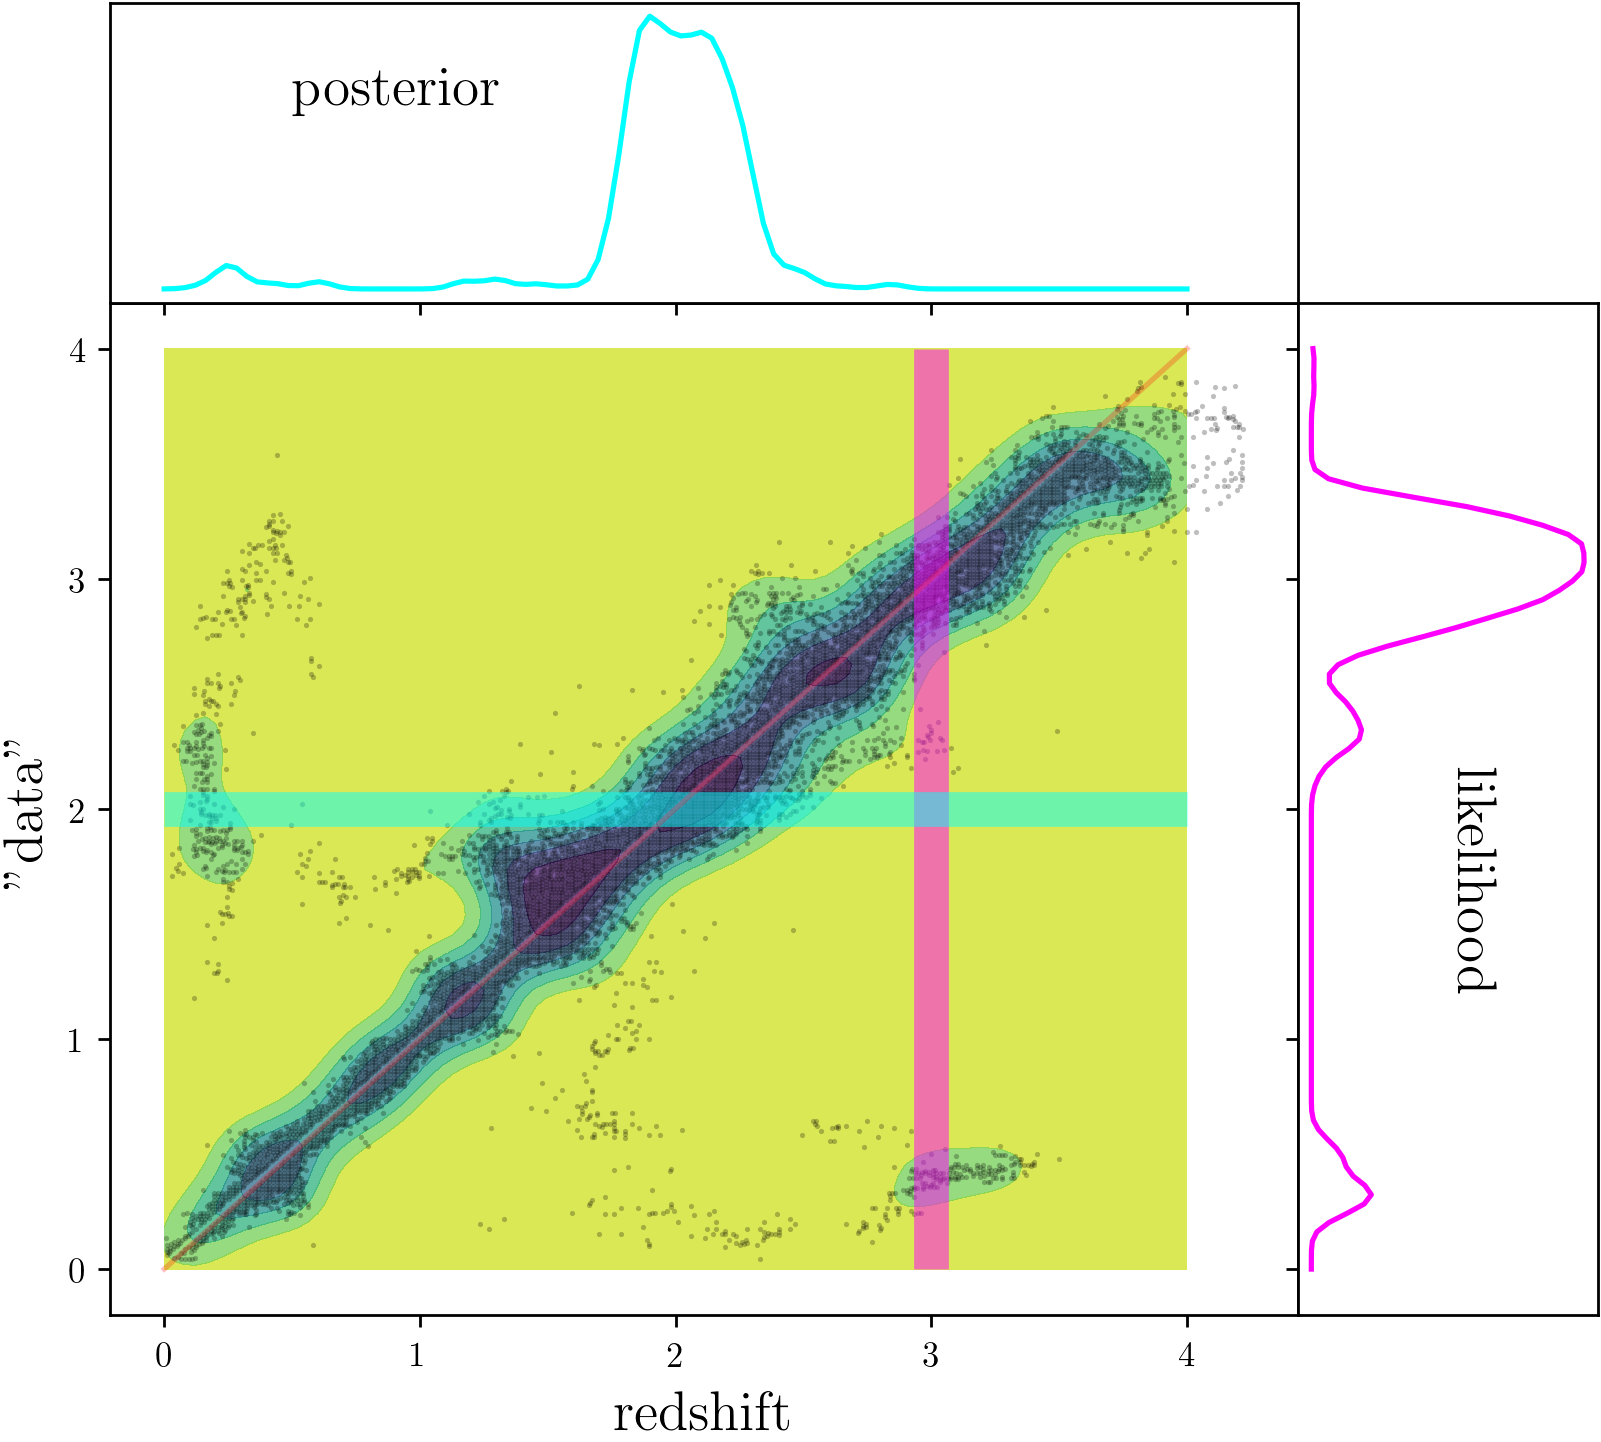
\includegraphics[width=0.45\textwidth]{figures/jain05.png}
		\caption{
			A generic probability space (darker in areas of higher probability density) of redshift ($x$-axis) and data ($y$-axis), where the data is projected into a single dimension, with vertical cuts and marginals (cyan) indicating the construction of likelihoods and horizontal cuts and marginals (magenta) indicating the construction of posteriors.
			The data (black points) used to generate the contours were extracted from \citet{jain_whole_2015} using WebPlotDigitizer \citep{rohatgi_webplotdigitizer_2019}, with the ideal redshift estimation provided for reference (red diagonal).
		}
		\label{fig:pedagogical_scatter}
	\end{center}
\end{figure}

% how do we interpret photo-z imperfections?
There are several varieties of generally non-Gaussian deviation from a \dwh{trivial relationship} between redshift and data in Figure~\ref{fig:pedagogical_scatter}, represented by a $y = x$ diagonal line.
The coarseness of the photometric filters causes scatter about the diagonal, with larger scatter perpendicular to the diagonal at redshifts where highly identifiable spectral features pass between the filters, as well as higher scatter at high redshifts where faint galaxies with large photometric errors are more abundant.
There are populations of outliers, far from the diagonal, comprised of galaxies for which the redshift estimate is catastrophically distinct from the true redshift, showing that outliers are not uniformly distributed nor restricted to long tails away from a Gaussian scatter.
And, though hardly perceptible in the plot, there is a systematic bias, wherein the average of the points would not lie on the diagonal but would be offset by a small bias, suggested by the trend of high-redshift points to lie below the diagonal.

% how much do these imperfections matter?
Once propagated through the calculations of correlation functions of cosmic shear and galaxy positions, \pz\ errors are a dominant contributor to the total uncertainties reported on cosmological parameters \citep{abruzzo_impact_2019}.
As progress has been made on the influence of other sources of systematic error, the uncertainties associated with \pz s have come to dominate the error budget of cosmological parameter estimates made by current surveys such as \des\ \citep{hoyle_dark_2017}, \project{HSC} \citep{tanaka_photometric_2018}, and \project{KiDS} \citep{hildebrandt_kids-450:_2017}.
Based on the goals of a photometric galaxy survey, limits can be placed on the tolerance to these effects.
For example, the Science Requirements Document \citep{mandelbaum_weak_2017} states \lsst's requirements for the main cosmological sample, reproduced in Table~\ref{tab:lsstsrd}.

\begin{table}
	\begin{center}
		\caption{\Pz\ requirements for \lsst\ cosmology\\
				\citep{mandelbaum_weak_2017}.}
		\begin{tabular}{ll}
			Number of galaxies & $\approx 10^{7}$\\
			Root-mean-square error & $< 0.02 (1 + z)$\\
			$3 \sigma$ catastrophic outlier rate & $< 10\%$\\
			Bias & $< 0.003 (1 + z)$\\
		\end{tabular}
		\label{tab:lsstsrd}
	\end{center}
\end{table}

% how can we improve photo-zs?
Much effort has been dedicated to improving \pz s, though they are still most commonly obtained by a maximum likelihood estimator (MLE) based on libraries of galaxy SED templates, with conservative approaches to error estimation.
The presence of galaxies whose SEDs are not represented by the template library tends to lead to catastrophic outliers distributed like the horizontally oriented population of \Fig{fig:pedagogical_scatter}.
For data-driven approaches, training sets that are incomplete in redshift coverage tend to result in catastrophic outliers like the vertically oriented population of \Fig{fig:pedagogical_scatter}.
The approaches of using a training set versus a template library are related to one another by \citet{budavari_unified_2009}.
Sophisticated Bayesian techniques and machine learning methods have been employed to improve precision \citep{carliles_random_2010} and accuracy \citep{sadeh_annz2:_2016}, while other advances have focused on identifying and removing catastrophic outliers when using \pz s for inference \citep{gorecki_new_2014}. 

% PDFs are a better way to improve photo-zs
\dwh{The probability density function (PDF) in redshift space for each galaxy, commonly written as $\pr{z}$, is an alternative to the MLE (with or without presumed Gaussian error bars) \citep{koo_photometric_1999}.}
This option is favorable because it contains more potentially useful information about the uncertainty on each galaxy's redshift, incorporating our understanding of precision, accuracy, and systematic error.
However, denoting \zpdf s as ``$\pr{z}$'' is an abuse of notation, as it does not adequately convey what information is being used to constrain the redshift $z$; \zpdf s are \textit{posterior} PDFs, conditioned on the photometric data and prior knowledge.
In terms of \Fig{fig:pedagogical_scatter}, \zpdf s are horizontal cuts, probabilities of redshift conditioned on a specific value of data, i.e. posteriors $\pr{z \gvn \data}$, which constrain redshifts, whereas vertical cuts through this space are probabilities of data conditioned on a specific redshift, i.e. likelihoods $\pr{\data \gvn z}$, from which photometric data is actually drawn.

% photo-z PDFs are established
\Pzpdf s have been produced by completed surveys \citep{hildebrandt_cfhtlens:_2012, sheldon_photometric_2012} and will be produced by ongoing and upcoming surveys \citep{abell_lsst_2009, carrasco_kind_exhausting_2014, bonnett_redshift_2016, masters_mapping_2015}.  
\Pzpdf s are not without their own shortcomings, however, including the resources necessary to calculate and record them for large galaxy surveys \citep{carrasco_kind_sparse_2014, malz_approximating_2018} and the divergent results of each method used to derive them \citep[ and reviewed in Schmidt, Malz \& Soo, et al. (in prep)]{hildebrandt_phat:_2010, dahlen_critical_2013, sanchez_clustering_2013, bonnett_redshift_2016, tanaka_photometric_2018}.  
The most concerning weakness of \pzpdf s, however, is their usage in the literature, which is at best inconsistent and at worst incorrect.  

% photo-z PDFs are most often reduced to point estimates
Though their potential to improve estimates of physical parameters is tremendous, \pzpdf s have been applied only to a limited extent, most often by reduction to familiar point estimates.
If the true redshifts $\{z_{j}^{\dagger}\}$ of galaxies $j$ are known, then their \dwh{redshift PDFs are well-approximated by delta functions} $\{\delta(z, z_{j}^{\dagger})\}$ centered at the true redshift\dwh{\footnote{\dwh{Note that \sz s are not the same as known true redshifts; the PDFs of \sz s would be narrow and almost always unimodal, but they would not be delta functions due to observational errors.}}}, and the redshift distribution is effectively approximated by a histogram or other interpolation of the delta functions $\{\delta(z, z_{j}^{\dagger})\}$.
When \pzpdf s are available instead of true redshifts, the simplest approach reduces them to point estimates $\{\hat{z}_{i}\}$ of redshift by using $\delta(z, \hat{z}_{j})$ in place of $\delta(z, z_{j}^{\dagger})$.
Though it is most common for $\hat{z}_{j}$ to be the maximum or \textit{mode} of the \pzpdf, there are other, more principled point estimate reduction procedures \citep{tanaka_photometric_2018}.

% photo-z PDFs may also be used to define cuts
Regardless of how it is done, any procedure that reduces \pzpdf s to point estimates discards valuable information about the uncertainty on redshift.
\Pzpdf s have also been used to form selection criteria of samples from galaxy surveys without propagation through the calculations of physical parameters \citep{van_breukelen_reliable_2009, viironen_high_2015}.  
Probability cuts on Bayesian quantities are not uncommon \citep{leung_bayesian_2017, dipompeo_quasar_2015}, but that procedure does not fully take advantage of all information contained in a probability distribution for parameter inference.

\aim{TODO: Provide equations/citations for the use of \Nz\ in cosmology, why it matters.}

The most prevalent application of \pzpdf s that preserves their information content is the estimation of the \textit{redshift distribution function \Nz}, or, interchangably, its normalized cousin the \textit{redshift density function \nz}.
\nz\ is used to calculate the redshift calibration bias $b_{z}$ between the true and observed critical surface densities in galaxy-galaxy lensing \citep{mandelbaum_precision_2008} and the geometric lens efficiency $g_{k}(\chi)$ in tomographic weak lensing by large-scale structure \citep{benjamin_cfhtlens_2013}.
The redshift distribution is a key input to the traditional calculation of the power spectra of weak gravitational lensing and large-scale structure that are used to constrain the parameters of cosmological models \citep{bonnett_using_2015,  masters_mapping_2015, viironen_high_2015, asorey_galaxy_2016, bonnett_redshift_2016, yang_calibrating_2018}.
\Nz\ may also be used to validate survey selection functions used in generation of realistic, multi-purpose mock catalogs \citep{norberg_2df_2002}.

\aim{TODO: Say what precision is needed for \Nz\ for future weak lensing surveys, motivate how well we need to know \Nz.}
Even with \pz s adhering to the \lsst\ requirements of \Tab{tab:lsstsrd}, the degree to which constraints on the cosmological parameters can advance is limited by the accuracy and precision to which \nz\ is known \citep{abruzzo_impact_2019}.
% Say what precision the mass function is needed (in, say cluster studies) for precision cosmology.

% how people get n(z) from photo-z PDFs
Though it is traditional to estimate \nz\ from \pz\ point estimates \citep{abruzzo_impact_2019}, there is a great deal of literature employing \pzpdf s.
To circumvent this loss, it has become more common to calculate the conceptually simple but mathematically inconsistent \citep{hogg_data_2012} \textit{stacked estimator} $\hat{n}(z)$ of the redshift density function \citep{lima_estimating_2008}
\begin{align}
\label{eqn:stack}
\hat{n}(z) &= \frac{1}{J} \sum_{j = 0}^{J} \pr{z}_{j}
\end{align}
for a sample of $J$ galaxies $j$, or, equivalently, the redshift distribution function $\hat{N}(z) = J \hat{n}(z)$, by effectively averaging the \pzpdf s.
This summation procedure has been used extensively \citep{mandelbaum_precision_2008, benjamin_cfhtlens_2013, kelly_weighing_2014}\aim{\dots}

% what this paper is about
Despite the growing prevalence of \pzpdf\ production, no implementation of inference using \pzpdf s has yet been presented with a mathematically consistent methodology.  
This paper challenges the logically invalid yet pervasive analysis procedure of stacking \pzpdf s by presenting and validating a hierarchical Bayesian technique for the use of \pzpdf s\ in the inference of \nz, yielding a method applicable to arbitrary one-point statistics relevant to cosmology, large-scale structure, and galaxy evolution; future work will extend this methodology to higher-order statistics.
We aim to develop a clear methodology guiding the use of \pzpdf s in inference so they may be utilized effectively by the cosmology community.
Though others have approached the problem before \citep{leistedt_hierarchical_2016, leistedt_hierarchical_2018}, the method presented here differs in that it makes use of any existing catalog of \pzpdf s, rather than requiring a simultaneous derivation of the \pzpdf s and the redshift distribution, making it preferable to ongoing surveys for which there may be inertia preventing a complete restructuring of the analysis pipeline.

In Section~\ref{sec:meth}, we present the \Chippr\ model and \chippr\ implementation for characterizing the full posterior probability landscape of \Nz\ using \pzpdf s. 
In Section~\ref{sec:alldata}, we describe the experimental design for testing the fully probabilistic approach to mock and real datasets, the results of which are found in Section~\ref{sec:results}.
In Section~\ref{sec:results}, we stress-test the \Chippr\ model against stacking and its other competitors in the context of cosmology.

\section{Method}
\label{sec:meth}

Consider a survey of $J$ galaxies $j$, each with photometric data $\data_{j}$; thus the entire survey over some solid angle produces the ensemble of photometric magnitudes (or colors) and their associated observational errors $\{\data_{j}\}$.  
Each galaxy $j$ has a redshift $z_{j}$ that we would like to learn; redshift is a parameter in this case.  
The distribution of the ensemble of redshifts $\{z_{j}\}$ may be described by the hyperparameters defining the redshift distribution function \nz\ that we would like to quantify.  
This situation may be considered to be a probabilistic generative model, illustrated by the directed acyclic graph of \Fig{fig:pgm}.  

The redshift distribution function \nz\ is the number of galaxies per unit redshift, effectively defining the evolution in the number of galaxies convolved with the selection function of the sample \citep{menard_clustering-based_2013}.  
In the following sections, we present and compare methods for estimating \nz\ from \pzpdf s.  
\Sect{sec:prob} contains the mathematical derivation of a probabilistic model for $n(z)$ dependent on photo-$z$ probability distribution functions, and \Sect{sec:sheldon} contrasts the probabilistic model with alternative methods.

\subsection{Forward Model}
\label{sec:forward}

We begin by reframing the redshift distribution \nz\ from a probabilistic perspective.
Here we define a redshift density \nz\ as the normalized probability density
\begin{equation}
\label{eqn:nz}
\int_{-\infty}^{\infty}\ n(z)\ dz\ \equiv\ \frac{1}{J}\ \int_{-\infty}^{\infty}\ \sum_{j=1}^{J}\ \delta(z_{j},\ z)\ dz = 1
\end{equation}
of finding a galaxy $j$ in a catalog of $J$ galaxies having a redshift $z$.
We believe that galaxy redshifts are indeed drawn from \nz, making it a probability density over redshift; this fact can also be confirmed by dimensional analysis of \Eq{eqn:nz}, as suggested in \citet{hogg_data_2012}.

We may without loss of generality impose a parameterization
\begin{equation}
\label{eqn:fz}
f(z; \ndphi)\ \equiv\ n(z)
\end{equation}
in terms of some parameter vector $\ndphi$.
At this point, the parameter vector is quite general and may represent coefficients in a high-order polynomial as a function of redshift, a set of means and variances defining Gaussians that sum to the desired distribution, a set of histogram heights that describe a binned version of the redshift distribution function, etc.
Upon doing so, we may rewrite \Eq{eqn:fz} as 
\begin{equation}
\label{eqn:pz}
z_{j}\ \sim\ \pr{z \gvn \ndphi}\ \equiv\ f(z; \ndphi),
\end{equation}
% \aim{explain "is drawn from"}
a probability density over redshift conditioned on the parameters $\ndphi$ specifying \nz.
Note that $z_{j}$ does not depend on the redshift $z_{j'}$ of some other galaxy $j' \neq j$, a statement of the causal independence of galaxy redshifts from one another.

In addition to believing \nz\ is a PDF from which redshifts are drawn, we also believe that there is some higher dimensional probability space $\pr{z, \data}$ of redshift and photometric data vectors $\data$, which may be any combination of fluxes, magnitudes, colors, and their observational errors.
In that sense \nz\ is equivalent to an integral
\begin{equation}
\label{eqn:integral}
n(z)\ =\ \integral{\pr{z, \data}}{\data}
\end{equation}
over the dimension of data in that joint probability space.
Note that galaxies may have different observational data despite sharing the same redshift, and that galaxies at different redshifts may have identical photometry; the space $\pr{z, \data}$ need not be one-to-one.
We assume a stronger version of statistical independence here, that draws $(z_{j}, \data_{j})$ are independent of draws $(z_{j'}, \data_{j'})$ in this space; the data and redshift of each galaxy are independent of those of other galaxies.

However, this problem has additional causal structure that we can acknowledge.
The photometry results from the redshifts, not the other way around.
This is the fundamental assumption upon which \pz\ estimation is based.
The forward model corresponds to first drawing redshifts according to \Eq{eqn:pz} and then drawing data from the likelihood
\begin{equation}
\label{eqn:pzpdf}
\data_{j}\ \sim\ \pr{\data \gvn z_{j}}
\end{equation}
of photometry conditioned on redshift, illustrated in Figure~\ref{fig:pedagogical_scatter}.

This description of the physical system corresponds to a forward model by which we actually believe photometry is generated:
\begin{enumerate}
	\item There exists a redshift distribution \nz\ with parameters $\ndphi$.
	\item Galaxy redshifts $\{z_{j}\}$ are independent draws from $\pr{z \gvn \ndphi}$.
	\item Galaxy photometry $\data_{j}$ is drawn from the likelihoods $\pr{\data_{j} \gvn z}$.
\end{enumerate}

\subsection{Probabilistic Model}
\label{sec:prob}

A forward model such as that of \Sect{sec:forward} corresponds to a probabilistic graphical model (PGM), represented by a directed acyclic graph (DAG) as in \Fig{fig:pgm}.
A DAG conveys the causal relationships between physical parameters and, like a Feynman diagram in the context of particle physics, is a shorthand for mathematical relationships between variables.
The photometric data $\data_{j}$ of a galaxy is drawn from some function of its redshift $z_{j}$, independent of other galaxies' data and redshift.
Both data and redshift are random variables, but data is the one that we observe and redshift is not directly observable.
In this problem, we don't care about further constraining the redshifts of individual galaxies, only the redshift distribution, so we consider redshift to be a \textit{latent variable}.
Because the parameters $\ndphi$ that we seek are causally separated from the data by the latent variable of redshift, we call them \textit{hyperparameters}.
\que{Am I adequately explaining the distinction between hyperparameters and parameters?}

\begin{figure}
	\begin{center}
		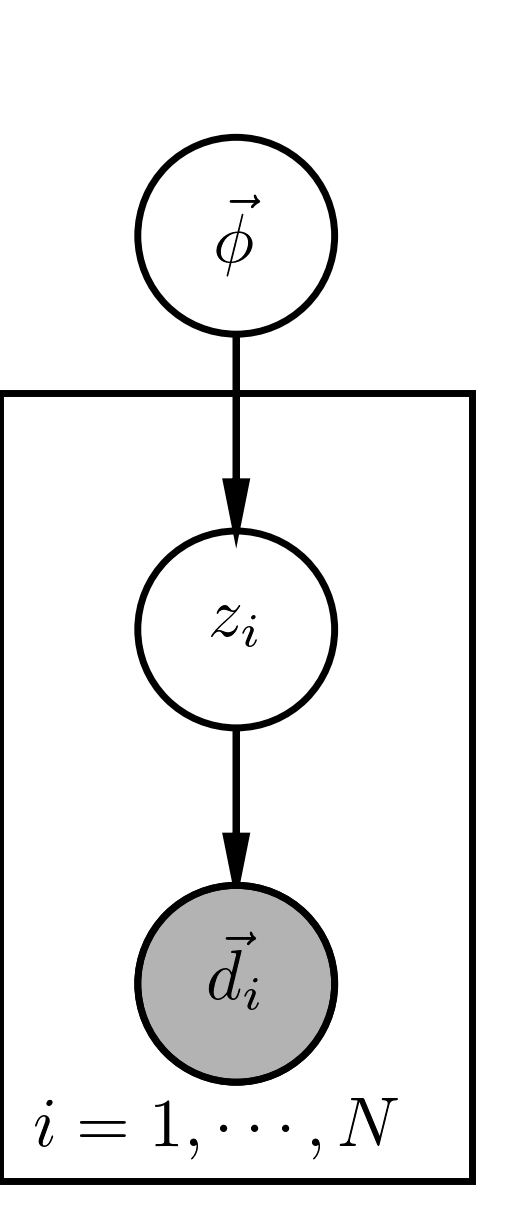
\includegraphics[height=0.25\textheight]{figures/chippr/pgm.png}
		\caption{The directed acyclic graph of the CHIPPR model, where circles indicate random variables and arrows indicate causal relationships.
			The redshift distribution \nz\ parameterized by hyperparameters $\ndphi$ exists independent of the survey of $J$ galaxies, indicated as a box.  
			The redshifts $\{z_{j}\}$ of all galaxies in the survey are latent variables independently drawn from the redshift distribution, which is a function of $\ndphi$. 
			The photometric data $\data_{j}$ for each galaxy is drawn from a function of its redshift $z_{j}$ and observed, indicated by a shaded circle.
			\aim{Switch to vector graphics version?}}
		\label{fig:pgm}
	\end{center}
\end{figure}

The problem facing cosmologists is to determine the true value of $\ndphi$ from observing the photometry $\{\data_{j}\}$ of a large sample of $J$ galaxies $j$.
To self-consistently propagate the uncertainty in the inference of redshift, however, it is more appropriate to estimate the posterior $\pr{\ndphi \gvn \{\data_{j}\}}$ over all possible values of $\ndphi$ conditioned on all the observed data $\{\data_{j}\}$ available in a generic catalog.
In order to use the DAG of \Fig{fig:pgm} to derive an expression for $\pr{\ndphi \gvn \{\data_{j}\}}$ in terms of \pzpdf s, we must introduce two more concepts, confusingly named the \textit{implicit prior} and the \textit{prior probability density (prior PDF)}, elaborated upon below.

\dwh{When we constrain the redshift of a galaxy using its observed photometric data $\data_{j}$, we are effectively estimating a posterior $\pr{z \gvn \data_{j}}$, the probability of an unknown quantity conditioned on the quantity we have in hand, i.e the data.
However, to do this, we must have a model for the general relationship between redshifts and photometry, whether empirical, as is the case for machine learning \pzpdf\ methods, or analytic, as is the case for template-based \pzpdf\ methods.
Such a relationship $\pr{\data, z}$ is defined in the multidimensional space of probability density over redshift and photometry.
If we were to marginalize over the photometry in $\pr{\data, z}$, we would obtain a one-dimensional PDF $\pr{z \gvn \ndphi^{*}}$ over redshift, which can by definition be parameterized by the same functional form as \nz, for some $\ndphi^{*}$ specific to the estimation procedure that may or may not bear any relation to the hyperparameters $\ndphi^{\dagger}$ of the true \nz.
Rather, $\ndphi^{*}$ is a consequence of generative model for how photometry results from redshift, including the influence of intrinsic galaxy spectra and instrumental effects. 
We call $\pr{z \gvn \ndphi^{*}}$ the \textit{implicit prior}, as it is rarely explicitly known nor chosen by the researcher\footnote{For template-based methods, the implicit prior is often an explicitly known input to the algorithm, engineered as an initial guess for the true $\ndphi$, with an aim for a realistic choice guided by an earlier spectroscopic survey.  
(See \citet{benitez_bayesian_2000} for more detail.)
It may thus be more appropriate to call it an \textit{interim prior}, but we will use the former term throughout this paper for generality.}
Because the implicit prior is unavoidable and almost inherently not uninformative, the \pzpdf s reported by any method must be \textit{implicit posteriors} $\pr{z \gvn \data, \ndphi^{*}}$ weighted by the implicit prior.}

%Posteriors differ from likelihoods by way of a prior distribution, so we cannot simply assume that the available data products are \pz\ posteriors $\pr{z \gvn \data_{j}}$.  
%Rather, we have a catalog of implicit-prior weighted \pz\ posteriors $\pr{z \gvn \data_{j}, \ndphi^{*}}$.  
%There must have been some interim prior probability distribution $p(z|\vec{\theta}^{*})$ defined in terms of the interim prior parameter values (hereafter the interim prior) $\vec{\theta}^{*}$ explicitly chosen or implicitly made to perform the calculation of the probabilistic photo-$z$s.  
%If it is implicit, it may not be representable in the parametrization we have chosen, and furthermore it may not be known at all; a method that produces interim photo-$z$ posteriors of this kind is not suitable for inference.  
%However, so long as the implicit prior is known, hierarchical inference is possible. 

The prior probability density $\pr{\ndphi}$ is a more familiar concept in astronomy; to progress, we will have to choose a prior probability density over all possible values of the hyperparameters $\ndphi$.
This prior need not be excessively proscriptive; for example, it may be chosen to enforce smoothness at physically motivated scales in redshift without imposing any particular region as over- or under-dense.

\dwh{With inputs of the \pzip\ catalog $\{\pr{z \gvn \data, \ndphi^{*}}\}$, the implicit prior $\pr{z \gvn \ndphi^{*}}$, and the prior PDF $\pr{\ndphi}$, we thus aim to obtain the posterior probability $\pr{\ndphi \gvn \{\data_{j}\}}$ of the redshift density function given all the photometric data.
By performing the derivation of Appendix~\ref{app:math}, we arrive at the desired expression
\begin{equation}
\label{eqn:fullpost}
\pr{\ndphi \gvn \{\data_{j}\}} \propto \pr{\ndphi} \integral{\prod_{j=1}^{J} \frac{\pr{z \gvn \data_{j}, \ndphi^{*}} \pr{z \gvn \ndphi}}{\pr{z \gvn \ndphi^{*}}}}{z},
\end{equation}
which is the very heart of \Chippr.
This in effect replaces the implicit prior with the sampled model hyperparameters, thereby converting the \pzip s into likelihoods in order to obtain unbiased posteriors.}

\subsubsection{Model Limitations}
\label{sec:limitations}

Finally, we explicitly review the assumptions made by this approach, which are as follows:
\begin{enumerate}
	\item Photometric measurements of galaxies are statistically independent Poisson draws from the set of all galaxies such that \Eq{eqn:indiedat} and \Eq{eqn:indie} hold.
	\item We take the reported \pzip s to be accurate, free of model misspecification; draws thereof must not be inconsistent with the distribution of photometry and redshifts.
	Furthermore, we must be given the implicit prior $\ndphi^{*}$ used to produce the \pzip s.
	\item We must assume a hyperprior distribution $\pr{\ndphi}$ constraining the underlying probability distribution of the hyperparameters, which is informed by our prior beliefs about the true redshift distribution function.
\end{enumerate}

These assumptions have known limitations.  
First, the photometric data are not a set of independent measurements; the data are correlated not only by the conditions of the experiment under which they were observed (instrument and observing conditions) but also by redshift covariances resulting from physical processes governing underlying galaxy spectra and their relation to the redshift distribution function.
Second, the reported \pzip s may not be trustworthy; there is not yet agreement on the best technique to obtain \pzpdf s, and the implicit prior may not be appropriate or even known to us as consumers of \pzip s.  
Third, the hyperprior may be quite arbitrary and poorly motivated if the underlying physics is complex, and it can only be appropriate if our prior beliefs about \nz\ are accurate.

\subsection{Implementation}
\label{sec:exp}

We implement the \Chippr\ model in code in order to perform tests of its validity and to compare its performance to that of traditional alternatives.
In \Sect{sec:mcmc}, we describe the publicly available \chippr\ library.
In \Sect{app:acorr}, we outline how \chippr\ can be used to sample the full log-posterior distribution $\ln[\pr{\ndphi \gvn \{\data_{j}\}}]$.

\subsubsection{Code}
\label{sec:mcmc}

\chippr\ is a \python\ 2 library\footnote{\url{https://github.com/aimalz/chippr}} that includes an implementation of the \Chippr\ model as well as an extensive suite of tools for comparing \Chippr\ to other approaches.

Though there are plans for future expansion to more flexible parameterizations, the current version of \chippr\ uses a log-space piecewise constant parameterization
\begin{equation}
\label{eqn:logstepfunc}
f(z; \ndphi) = \exp[\phi^{k}]\ \mathrm{if}\ z^{k} < z < z^{k+1}
\end{equation}
for \nz\ and every \pzpdf, satisfying
\begin{equation}
\label{eqn:logstepfuncnorm}
\sum_{k=1}^{K} \exp[\phi^{k}] \delta z^{k} = 1
\end{equation}
with $K$ bins of width $\delta z^{1}, \dots, \delta z^{K}$ defined by endpoints $z^{0}, \dots, z^{K}$.
%\aim{Maybe include an equation for a general piecewise constant function here (which is currently in \Chap{qp})?}
Thus each $\pr{z \gvn \data_{j}} = f(z; \ndphi_{j})$ has parameters $\ndphi_{j}$ that are defined in the same basis as those of \nz.
To infer the full log-posterior distribution $\ln[\pr{\ndphi \gvn \{\data_{j}\}}]$, one must provide a plaintext file with $K+1$ redshift bin endpoints $\{z_{k}\}$, the parameters $\ndphi^{*}$ of the implicit log-prior, and the parameters $\{\ndphi_{j}\}$ of the log-posteriors $\ln[\pr{z \gvn \data_{j}, \ndphi^{*})}$.

The \emcee \citep{foreman-mackey_emcee_2013} implementation of ensemble sampling is used to sample the full log-posterior of \Eq{eqn:final}. 
\chippr\ accepts a configuration file of user-specified parameters, among them the number $W$ of walkers.
At each iteration $i$ and for each walker, a proposal distribution $\hat{\ndphi}_{i}$ is drawn from the log-prior distribution and evaluated for acceptance to or rejection from the full log-posterior distribution.

Two threshold conditions are defined, one designating all previous samples to be ignored as as products of a burn-in phase and another indicating when a sufficient number of post-burn samples have been accepted.  
In this case, the first threshold (described in \Sect{app:acorr}) is defined in terms of sub-runs of $10^{3}$ accepted samples, and the second is defined as an accumulation of $10^{4}$ samples.

%Though previous versions used \texttt{HDF5} for the primary I/O format due to its efficiency for large quantities of data, it was abandoned in favor of \texttt{pickle} in the working release due to the instability of the \python\ implementation of the format on high-performance computing systems.  
The resulting output is a set of $I$ ordered \texttt{pickle} files enumerated by $\rho$ containing the state information after each sub-run.  
The state information includes $\frac{I_{0}}{s}$ actual samples $\ndphi_{i}$ for a pre-specified chain thinning factor $s$ and their full posterior probabilities $\pr{\ndphi_{i} \gvn \{\data_{j}\}}$ as well as the autocorrelation times and acceptance fractions calculated for each element of $\ndphi$ over the entire sub-run.  

\subsection{Comparison with Alternative Approaches}
\label{sec:sheldon}

In this study, we compare the results of \Eq{eqn:fullpost} to those of the two most common approaches to estimating \nz\ from a catalog of \pzpdf s: the distribution $n(z_{\mathrm{max}})$ of the redshifts at maximum posterior probability
\begin{equation}
\label{eqn:mmap}
f^{MMAP}(z; \hat{\ndphi}) = \sum_{j=1}^{J}\ \delta(z, \mathrm{mode}[\pr{z \gvn \data_{j}, \ndphi^{*}}])
\end{equation}
(i.e. the distribution of modes of the \pzpdf s) and the stacked estimator of \Eq{eqn:stacked}, which can be rewritten as 
\begin{equation}
\label{eqn:stacked}
f^{stack}(z; \hat{\ndphi}) = \sum_{j=1}^{J}\ \pr{z \gvn \data_{j}, \ndphi^{*}}
\end{equation}
in terms of the implicit \pz\ posteriors we have.
These two approaches have been compared to one another by \citet{hildebrandt_cfhtlens:_2012}, \citet{benjamin_cfhtlens_2013}, and \citet{asorey_galaxy_2016} in the past but not to \Chippr.

Point estimation converts the implicit photo-$z$ posteriors $\pr{z \gvn \data_{j}, \ndphi^{*}}$ into delta functions with all probability at a single estimated redshift.  
Some variants of point estimation choose this single redshift to be that of maximum a posteriori probability $\mathrm{mode}[\pr{z \gvn \data_{j}, \ndphi^{*}}]$ or the expected value of redshift $\langle z \rangle = \integral{z \pr{z \gvn \data_{j}, \ndphi^{*}}}{z}$.
\citet{tanaka_photometric_2018} directs attention to deriving an optimal point estimate reduction of a \pzpdf, but since the purpose of this paper is to compare against the most established alternative estimators of \nz, its use will be postponed until a future study.
Stacking these modified \pzpdf s leads to the marginalized maximum a posteriori (MMAP) estimator and the marginalized expected value (MExp) estimator, though only the former is included in this study since the latter has fallen out of favor in recent years\footnote{And for good reason!  Consider a bimodal \pzpdf; its expected value may very well fall in a region of very low probability, yielding a less probable point estimate than the point at which either peak achieves its maximum.}.

It is worth discussing the relationship between point estimation and stacking.  
When the point estimator of redshift is equal to the true redshift, stacking delta function \pzpdf s will indeed lead to an accurate recovery of the true redshift distribution function.  
However, stacking is in general applied indiscriminately to broader \pzpdf s and imperfect point estimators of redshift.  
It is for these reasons that alternatives are considered here.

A final estimator of the hyperparameters is the maximum marginalized likelihood estimator, the value of $\ndphi$ maximizing the log posterior given by \Eq{eqn:final} using any optimization code.  
To compare with sampling, the MMLE also depends on the choice of the hyperprior distribution, and it does not produce a full posterior probability distribution over the parameters of interest, only point estimators.  
It must be noted that computation of the maximum marginalized likelihood estimator may be unstable depending on the strengths and weaknesses of the optimizer.  
In general, derivatives will not be available for the full posterior distribution, restricting optimization methods used.
%\begin{equation}
%\label{eq:mmle}
%\ln[p(\{\vec{d}_{j}\}|\vec{\theta})] \propto -\int\ f_{\vec{\theta}}(z)\ 
%dz+\sum_{j=1}^{J}\ln\left[\int\ 
%\exp\left[\ln[p(z_{j}|\vec{d}_{j},\vec{\theta}^{*})]+\ln[f_{\vec{\theta}}(z)]-\l
%n[f_{\vec{\theta}^{*}}(z)]\right]\ dz\right],
%\end{equation}
%accessible with any optimization code.

In \Sect{sec:diag} we outline the measures used to evaluate the performance of the method.

\subsubsection{Performance metrics}
\label{sec:diag}

The results of the computation described in \Sect{sec:mcmc} are evaluated for accuracy on the basis of some quantitative measures.  
Beyond visual inspection of samples, we calculate summary statistics to quantitatively compare different estimators' precision and accuracy.  
Since MCMC samples of hyperparameters are Gaussian distributions, we can quantify the breadth of the distribution for each hyperparameter using the standard deviation regardless of whether the true values are known.  

In simulated cases where the true parameter values are known, we calculate the Kullback-Leibler divergence (KLD), given by 
\begin{equation}
\label{eqn:kl}
KL_{',\ddagger} = \integral{\pr{z \gvn \ndphi'} \ln \left[ \frac{\pr{z \gvn \ndphi'}}{\pr{z \gvn \ndphi^{\dagger}}} \right]}{z} ,
\end{equation}
which measures a distance from parameter values $\ndphi'$ to true parameter values $\ndphi^{\dagger}$, which is invariant under changes of variables.  
We note that $KL_{',\dagger} \neq KL_{\dagger,'}$ and is only interpretable when there is a notion that $\ndphi^{\dagger}$ is closer to the truth than $\ndphi'$.
The KLD is explored in detail in the Appendix to \citet{malz_approximating_2018}.
In simulated tests, $\ndphi^{\dagger}$ is the true value and $\ndphi'$ is that produced by one of the methods in question.

\section{Validation}
\label{sec:alldata}

We compare the results of \Chippr\ to those of stacking and the histogram of \pzpdf\ maxima (modes) on mock data in the form of catalogs of emulated \pzpdf s generated via the forward model discussed in \Sect{sec:forward}.
\dwh{\Fig{fig:flowchart} illustrates the implementation of the forward model, defined by the much simpler \Fig{fig:pgm}, used for validating the method presented here.
The irony of a simple model and complex validation procedure is not lost on the authors.}

\dwh{\Fig{fig:flowchart} outlines the four phases of the generative model, which uses a total of three inputs.
The experimental design requires our choice of true values $\phi^{\dagger}$ of the hyperparameters governing \nz, a \pz\ model $\pr{z, \data}$ defining the space of redshift and photometry, and prior values $\phi^{*}$ of the hyperparameters of \nz.
In the first phase, we sample $J = 10^{4}$ redshifts $z_{j}^{\dagger} \sim \pr{z \gvn \phi^{\dagger}}$.
In the second phase, we evaluate the \pz\ model at those redshifts, yielding a set of $J$ likelihoods $\pr{\data \gvn z_{j}^{\dagger}}$, from which we then sample data $\data_{j}^{\dagger} \sim \pr{\data \gvn z_{j}^{\dagger}}$ for each galaxy.
In the third phase, we evaluate the \pz\ model at that data to obtain $J$ posteriors $\pr{z \gvn \data_{j}^{\dagger}}$.
In the fourth phase, we convolve the posteriors with the chosen prior $\pr{z \gvn \phi^{*}}$, yielding implicit posteriors $\pr{z \gvn \data_{j}^{\dagger}, \phi^{*}}$.}

\begin{figure*}
	\begin{center}
		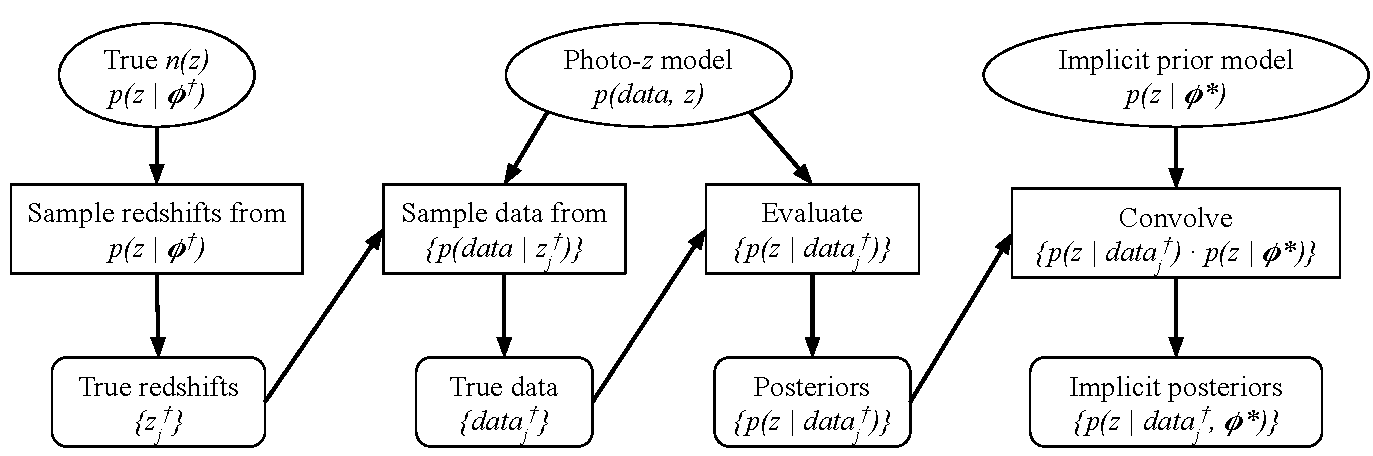
\includegraphics[width=0.9\textwidth]{figures/chippr/flowchart.pdf}
		\caption{
			\que{How to make this more attractive?}
			A flow chart illustrating the forward model used to generate mock data in the validation of \Chippr, as described in \Sect{sec:forward}.
			Ovals indicate a quantity that must be chosen in order to generate the data, rectangles indicate an operation we perform, and rounded rectangles indicate a quantity created by the forward model.
			Arrows indicate the inputs and outputs of each operation performed to simulate mock \pzpdf\ catalogs.
			}
		\label{fig:flowchart}
	\end{center}
\end{figure*}

The true redshift distribution used in these tests is a particular instance of the gamma function
\begin{equation}
\label{eqn:gamma}
n^{\dagger}(z) = \frac{1}{2 c_{z}} \left(\frac{z}{c_{z}}\right)^{2}\ \exp\left[-\frac{z}{c_{z}}\right]
\end{equation}
with $c_{z} = 0.3$, because it has been used in forecasting studies for \des\ and \lsst.
%\aim{I learned this from talking to people and don't know of a published source that talks about the nitty gritty of the internal validation tests performed before there was data.}

The mock data emulates the three sources of error of highest concern to the \pz\ community that are explored in detail later in this section: intrinsic scatter (\Sect{sec:scatter}), catastrophic outliers (\Sect{sec:outliers}), and systematic bias (\Sect{sec:bias}).
Tests including all three effects at the tolerance levels of \lsst\ (see Table~\ref{tab:lsstsrd}) 
are presented in \Sect{sec:results}.
\Fig{fig:mega_scatter} illustrates these three effects individually at twice the tolerance of \lsst\ for demonstrative purposes, hearkening back to Figure~\ref{fig:pedagogical_scatter}.
We also test nontrivial implicit priors in \Sect{sec:interim}, which ought to be a priority for the \pz\ community.

\begin{figure*}
	\begin{center}
		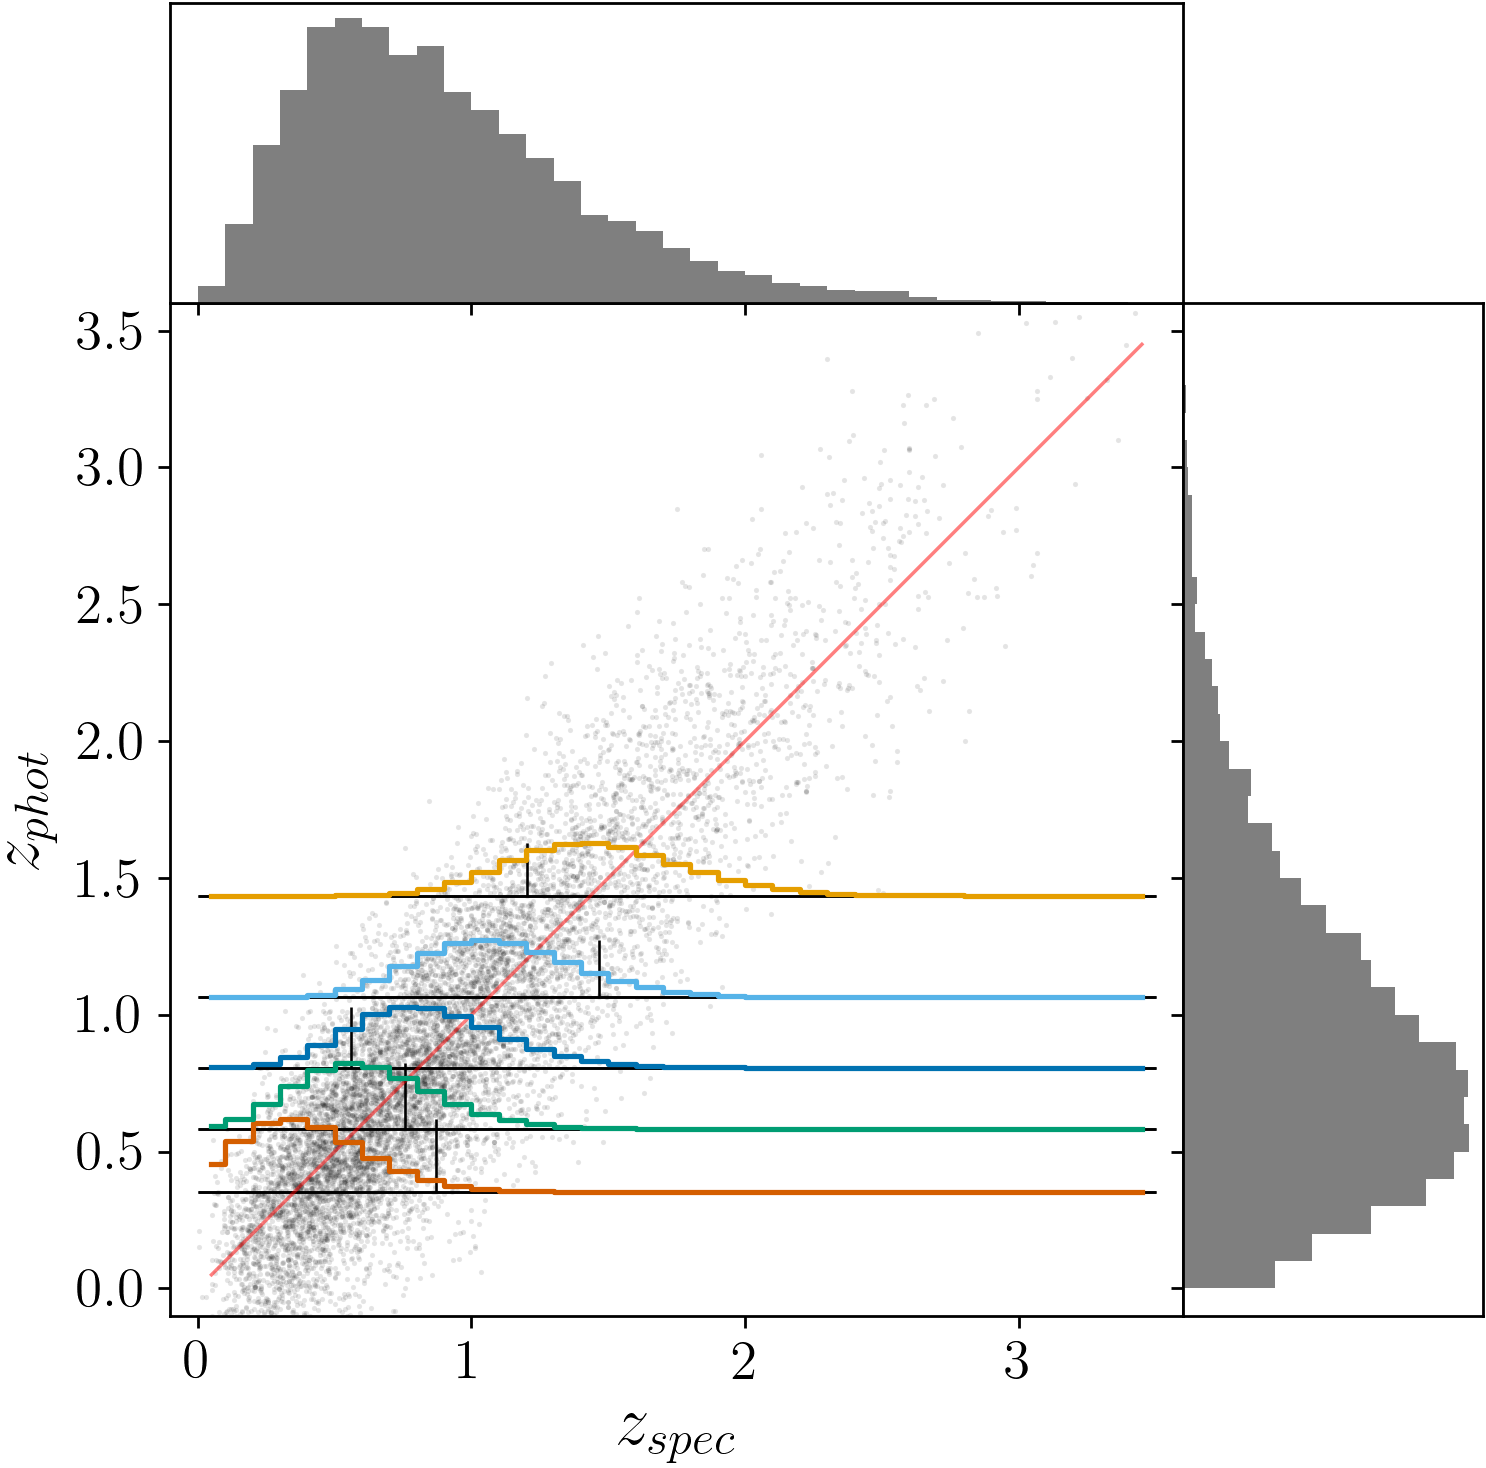
\includegraphics[width=0.32\textwidth]{figures/chippr/thesis_hivarsig-mega_scatter.png}
		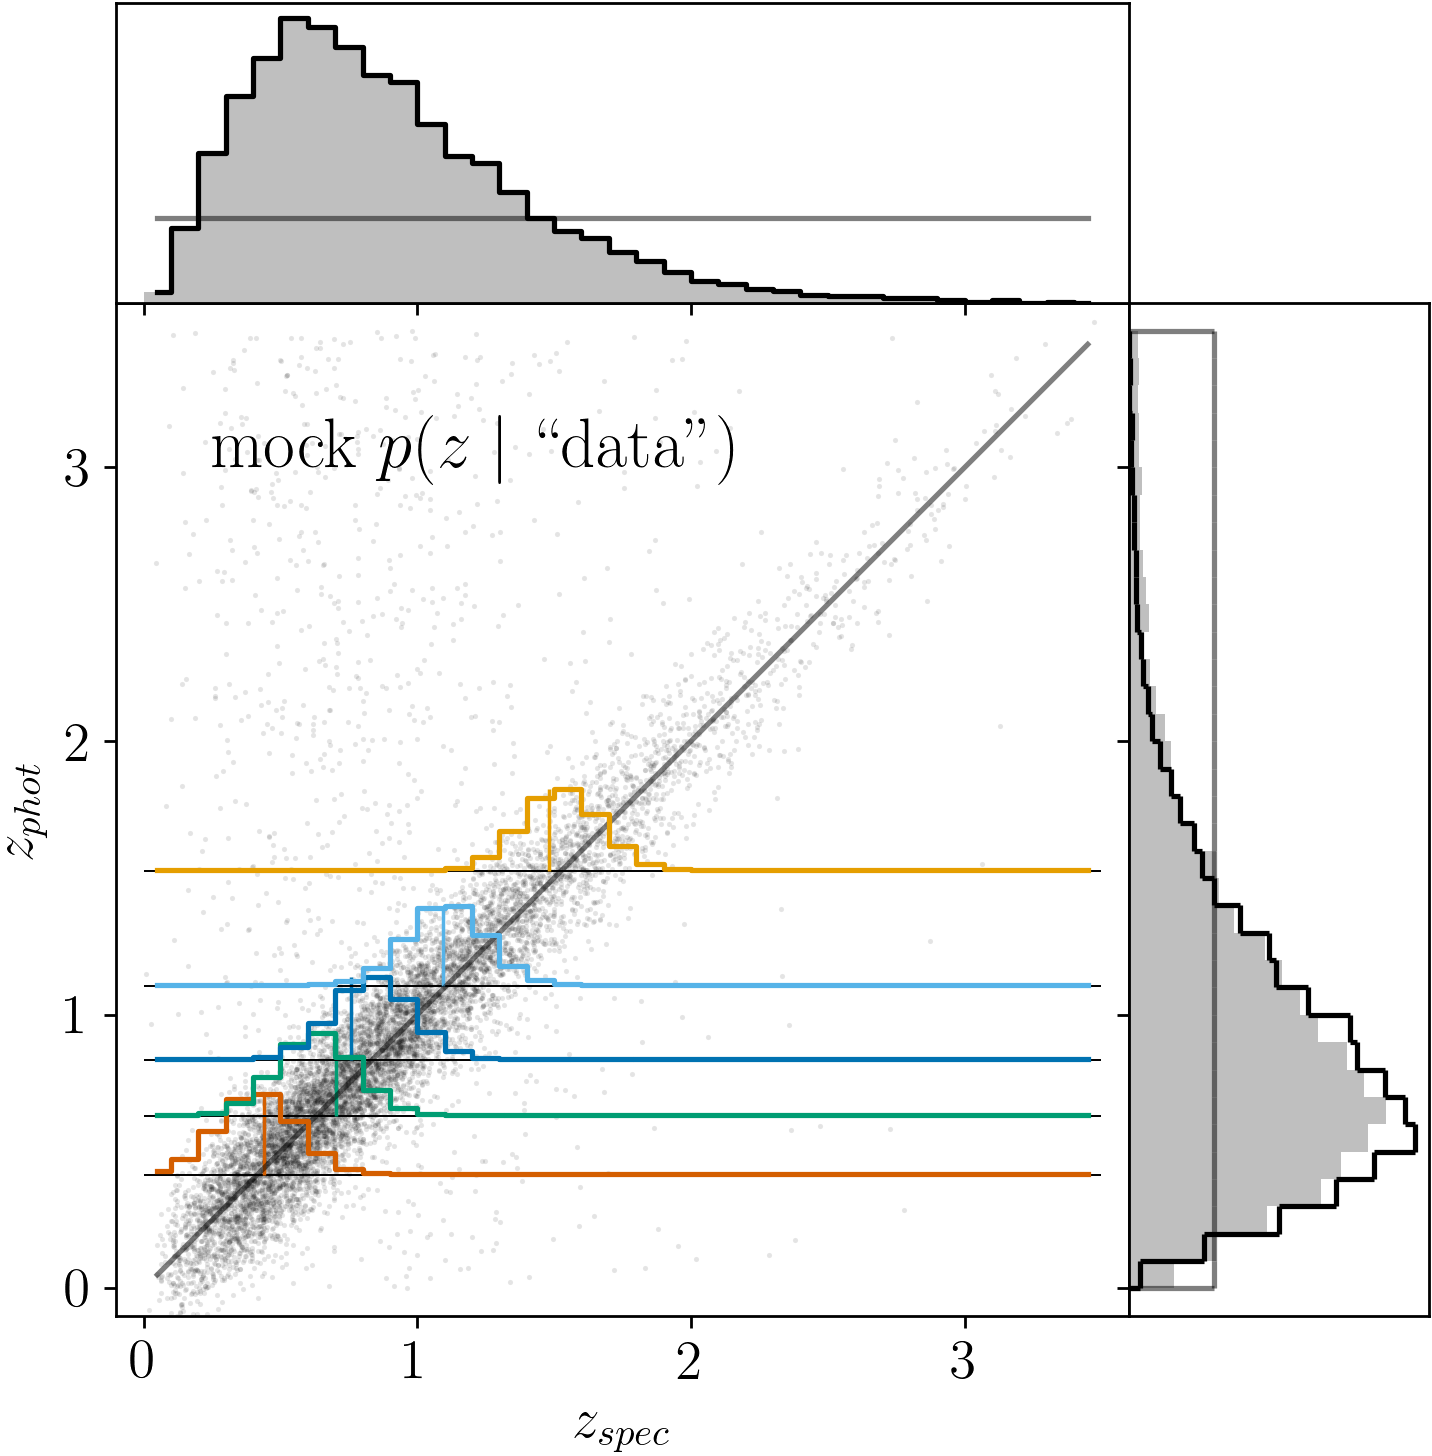
\includegraphics[width=0.32\textwidth]{figures/chippr/single_uout-mega_scatter.png}
		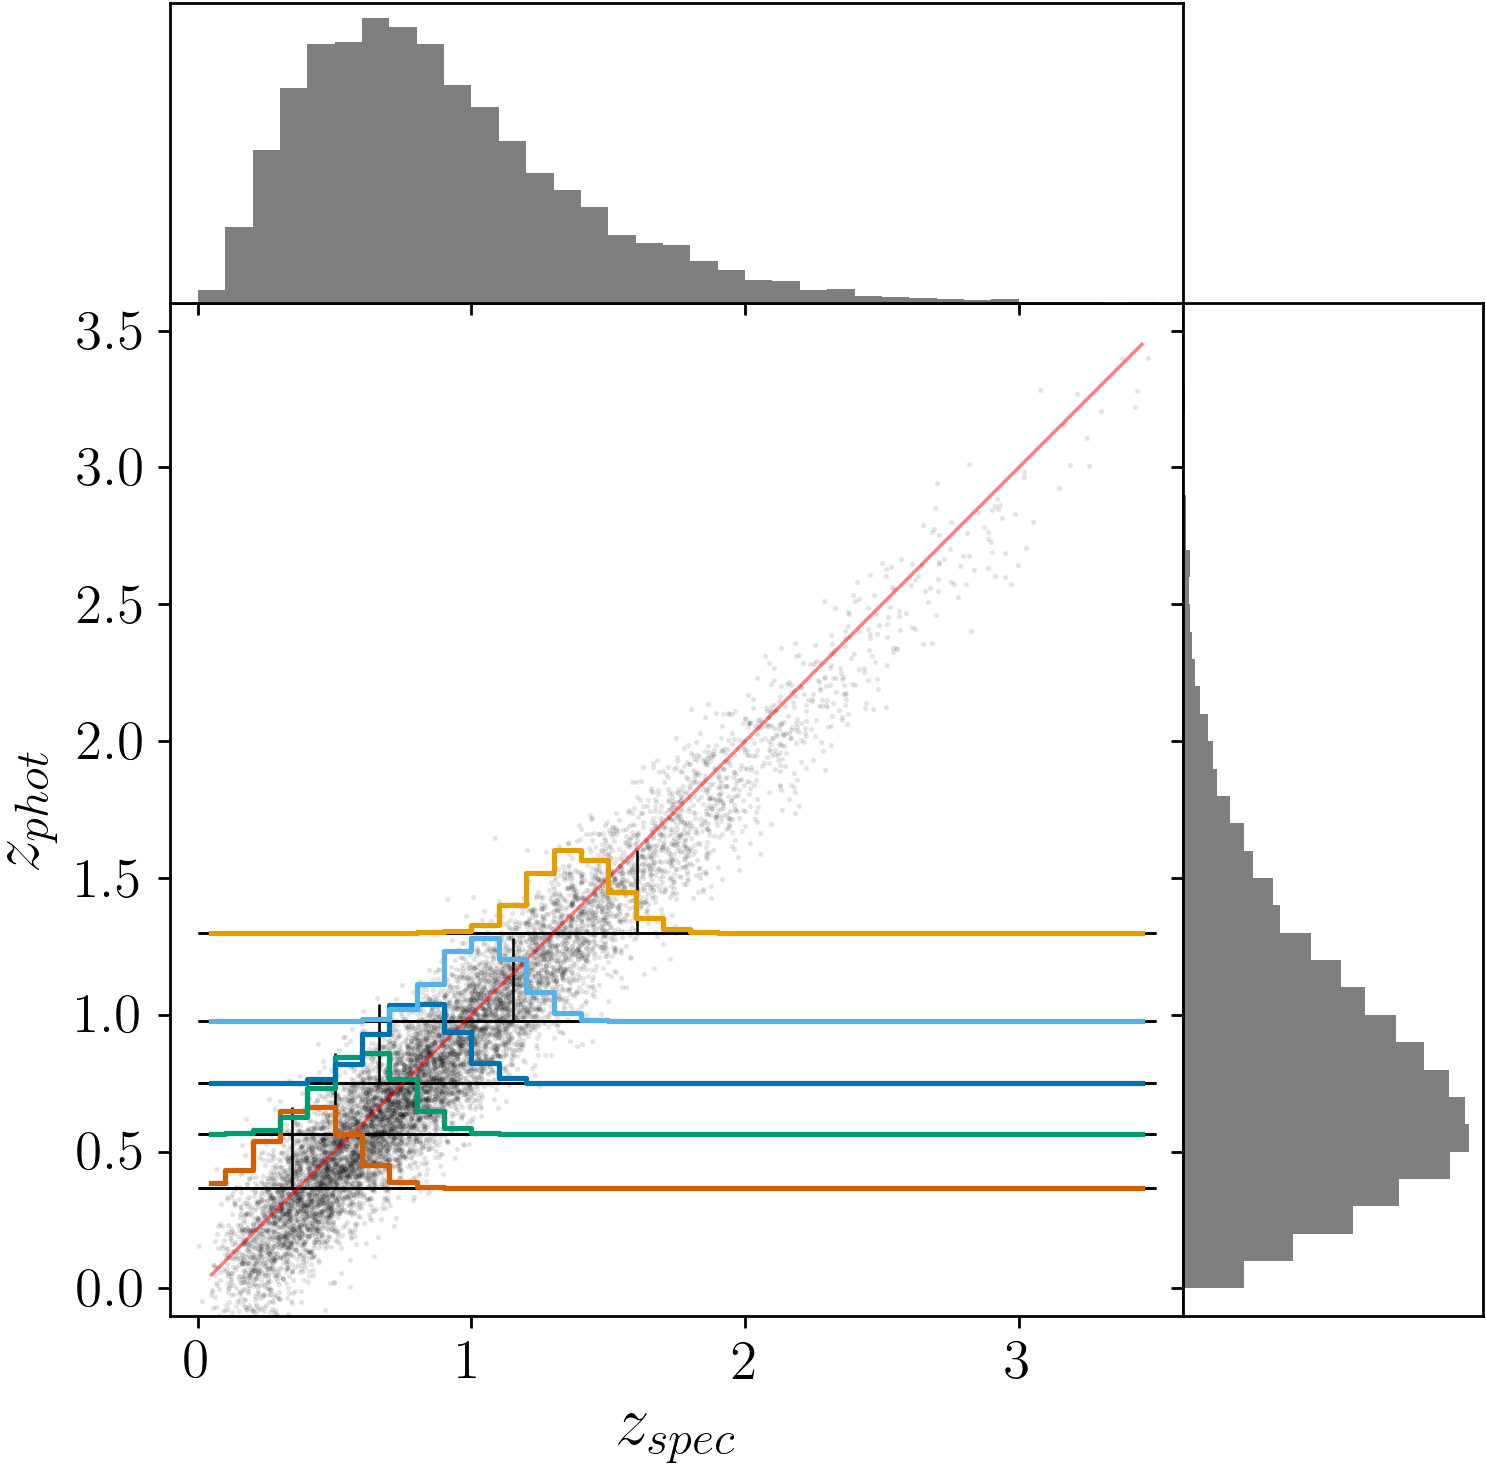
\includegraphics[width=0.32\textwidth]{figures/chippr/thesis_neghivarbias-mega_scatter.png}
		\caption{The joint probability space of true and estimated redshift for the three concerning \pz\ systematics at twice the level of the \lsst\ requirements: intrinsic scatter (left), uniform outliers (center), and bias (right).
			The main panel of each shows samples (black points) in the space of mock data and redshift, akin to the standard scatterplots of true and estimated redshift, the $z_{\mathrm{true}} = z_{\mathrm{phot}}$ diagonal (thin red line), and posterior probabilities evaluated at the given estimated redshift (colored step functions).
			The insets show marginal histograms (gray) in each dimension that can be compared with the true \nz\ (blue curve) used to make the figure to see the effect of the isolated systematic, as well as the implicit prior (red line).
			\aim{TODO: Omit this figure; redundant with right panel of \Fig{fig:pzs-scatter} and top panels of \Fig{fig:uniform-outliers} and \Fig{fig:bias}.}
%%			Enlarge axis labels and label panels.}
%%			Add watermark of ``mock data'' in UL corner, same for ``results of inference'' on other kind of plot.}
		}
		\label{fig:mega_scatter}
	\end{center}
\end{figure*}

The hyperprior distribution chosen for these tests is a multivariate normal distribution with mean $\vec{\mu}$ equal to the implicit prior $\ndphi^{*}$ and covariance
\begin{equation}
\label{eqn:priorcov}
\Sigma_{k,k'} = q\ \exp[-\frac{e}{2}\ (\bar{z}_{k}-\bar{z}_{k'})^{2}]\ +\ t\delta(k,k')
\end{equation}
inspired by one used in Gaussian processes, where $k$ and $k'$ are indices ranging from $1$ to $K$ and $q=1.0$, $e=100.0$, and $t=q\cdot10^{-5}$ are constants chosen to permit draws from this prior distribution to produce shapes similar to that of a true $\tilde{\ndphi}$.  
We adapt the full log-posterior of \Eq{eqn:final} to the chosen binning of redshift space.

%An example of such samples from the prior are shown in \Fig{fig:prior}.
%
%\begin{figure}
%%	\includegraphics[width=0.5\textwidth]{figures/chippr/null_priorsamps.pdf}
%	\caption{\aim{I need to remake this one because it uses the wrong notation and I stopped making it automatically a while ago.}
%		Samples (colored lines) of $\pr{z \gvn \ndphi}$ where each $\ndphi$ is drawn from the hyperprior distribution $\pr{\ndphi}$ given in \Eq{eqn:priorcov}.}
%	\figlabel{fig:prior}
%\end{figure}
\que{Should I add back the figure of prior samples?}

The sampler is initialized with $W=100$ walkers each with a value chosen from a Gaussian distribution of identity covariance around a sample from the hyperprior distribution.  

\subsection{Intrinsic scatter}
\label{sec:scatter}

%Several factors contribute to photometric redshifts' intrinsic scatter.  
%Distant galaxies are dimmer compared to galaxies of identical luminosity that are closer, driving up photometric errors in flux-limited surveys.  
%The nature of the galaxy sample at higher redshifts also changes, meaning the generation of the photometric redshift posterior based on an a locally-calibrated SED template library or spectroscopically-confirmed training set is more likely to be inappropriate, leading to broader features.  
%In general, the galaxies that could not have been observed spectroscopically will have different and noisier photo-$z$ likelihoods than those that could fall into a spectroscopic training set (or spectroscopically derived template library).  
%This effect may be stronger for high-redshift galaxies.  

\Fig{fig:pzs-scatter} shows some examples of \pzpdf s generated with only the systematic of intrinsic scatter, at the level of the \lsst\ requirements on the left and twice that on the right.
One can see that the histogram of redshift estimates is broader than that of true redshifts, and that the effect is substantially more pronounced by just doubling the intrinsic scatter from the level of the \lsst\ requirements.

\begin{figure*}
	\begin{center}
	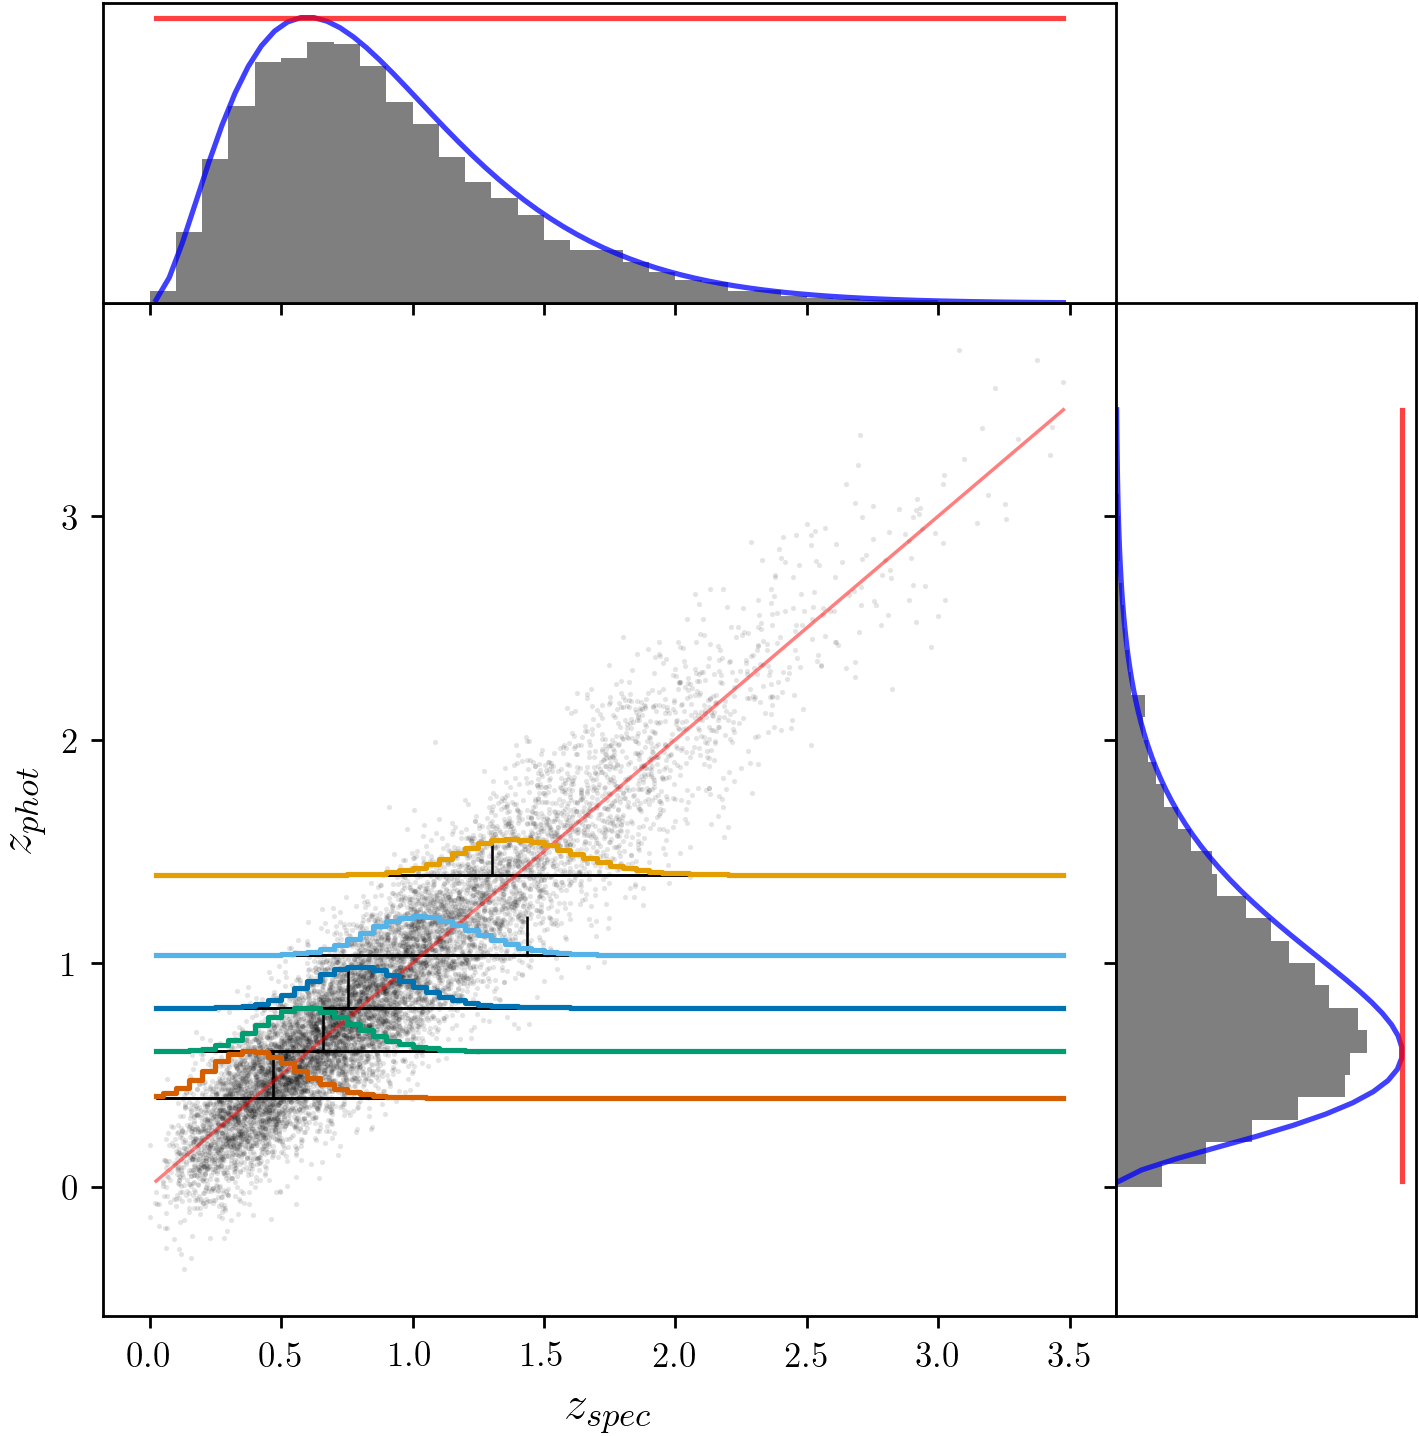
\includegraphics[width=0.45\textwidth]{figures/chippr/samplepzs_scatter1.png}
	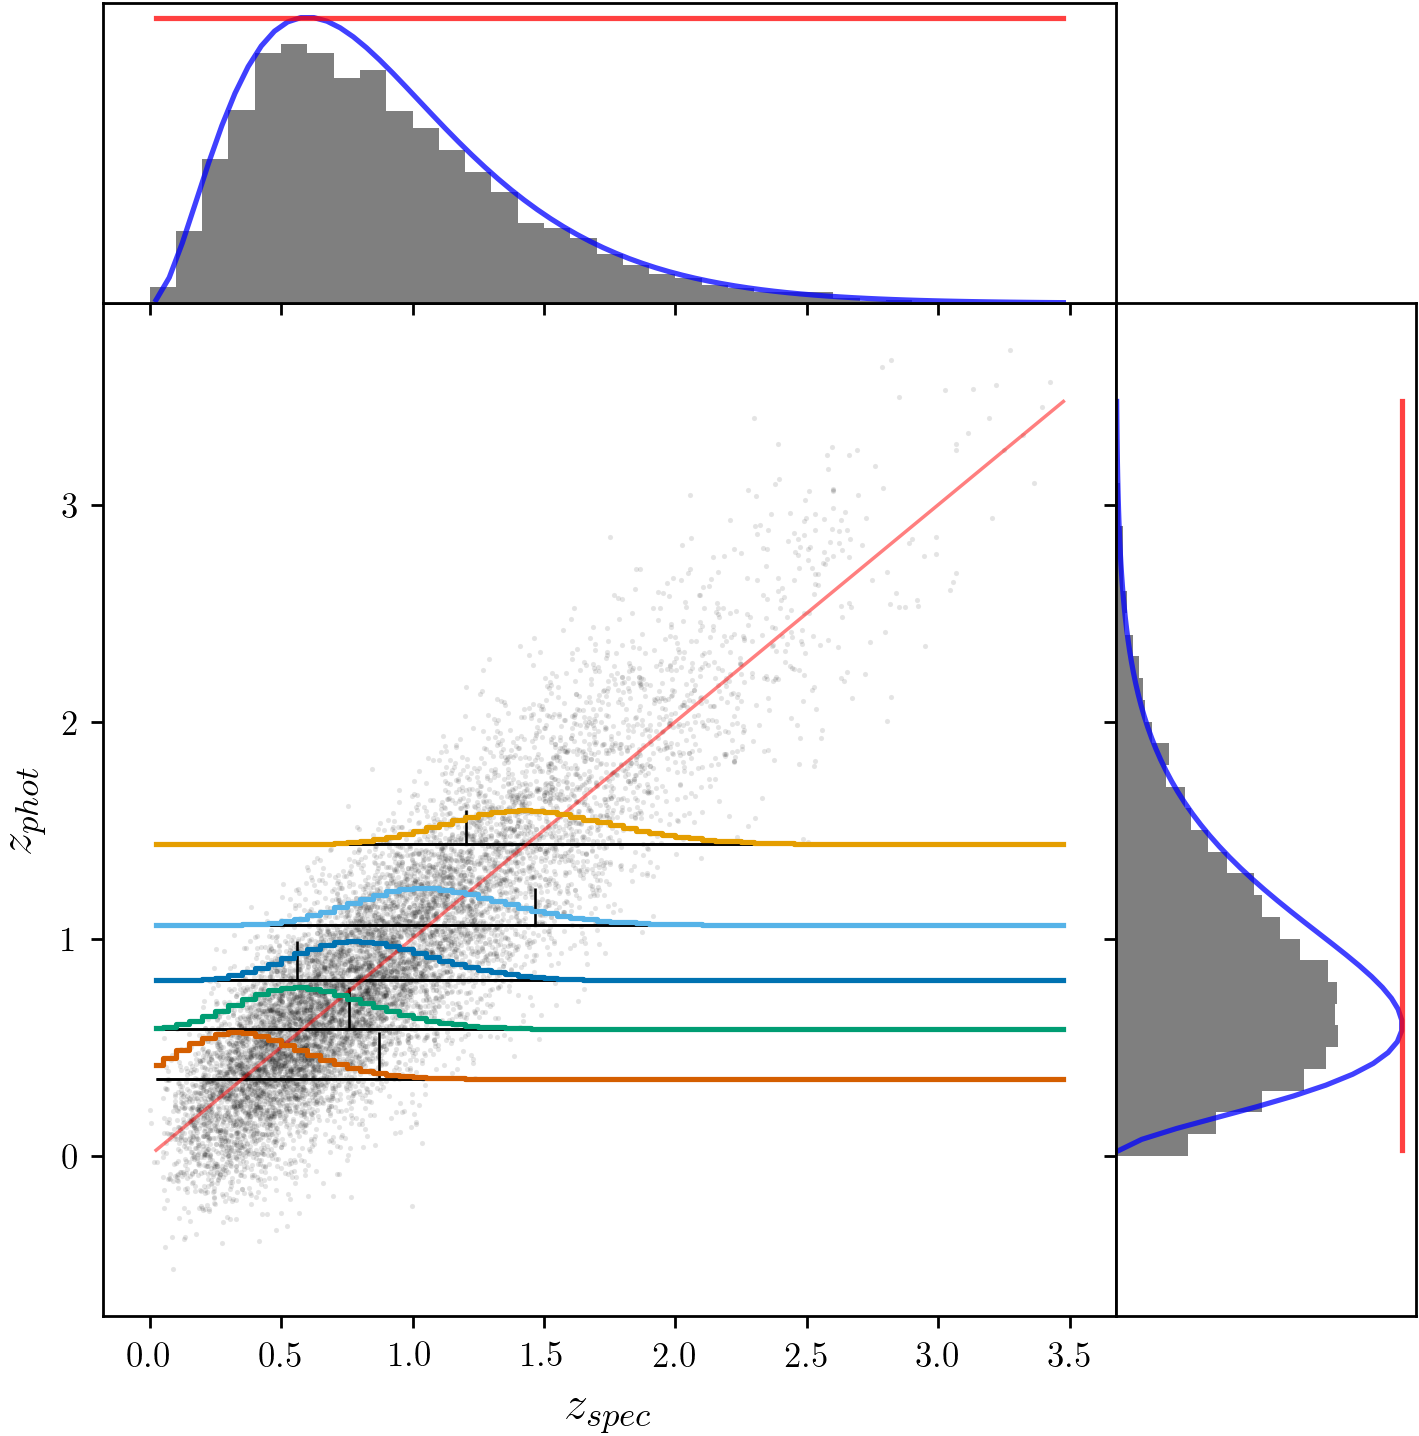
\includegraphics[width=0.45\textwidth]{figures/chippr/samplepzs_scatter2.png}
	\caption{
		Examples of mock \pzpdf s (colored lines) generated with intrinsic scatter at the \lsst\ requirements (left) and twice the \lsst\ requirements (right), including samples from the probability space of true and observed redshift (black points), \pzpdf s (colored lines), the true redshifts of the example \pzpdf s (black vertical lines).
		A histogram (gray) of points in each dimension is shown in the respective inset, with the true redshift distribution (blue curve) and implicit prior (red curve).
		\aim{TODO: Enlarge axis labels and label panels.
		Add watermark of ``mock data'' in UL corner, same for ``results of inference'' on other kind of plot.}
	}
	\label{fig:pzs-scatter}
	\end{center}
\end{figure*}

\Fig{fig:results-scatter} shows the \nz\ recovered by \Chippr\ and the alternative approaches.
As expected, the estimates of \nz\ based on the modes of the \pzpdf s and stacking are broader than the marginalized maximum likelihood estimator from \chippr, with more broadening as the intrinsic scatter increases.
\Chippr's \mmle\ is robust to intrinsic scatter and is unaffected by increased intrinsic scatter, though the \Chippr\ posterior distribution on the redshift distribution is itself broader for the higher intrinsic scatter case than for the \lsst\ requirements.
The broadening of the alternative estimators corresponds to a loss of 3-4 times as many nats of information about \nz\ for the \lsst\ requirements relative to the \mmle\ of \Chippr.

\begin{figure*}
	\begin{center}
	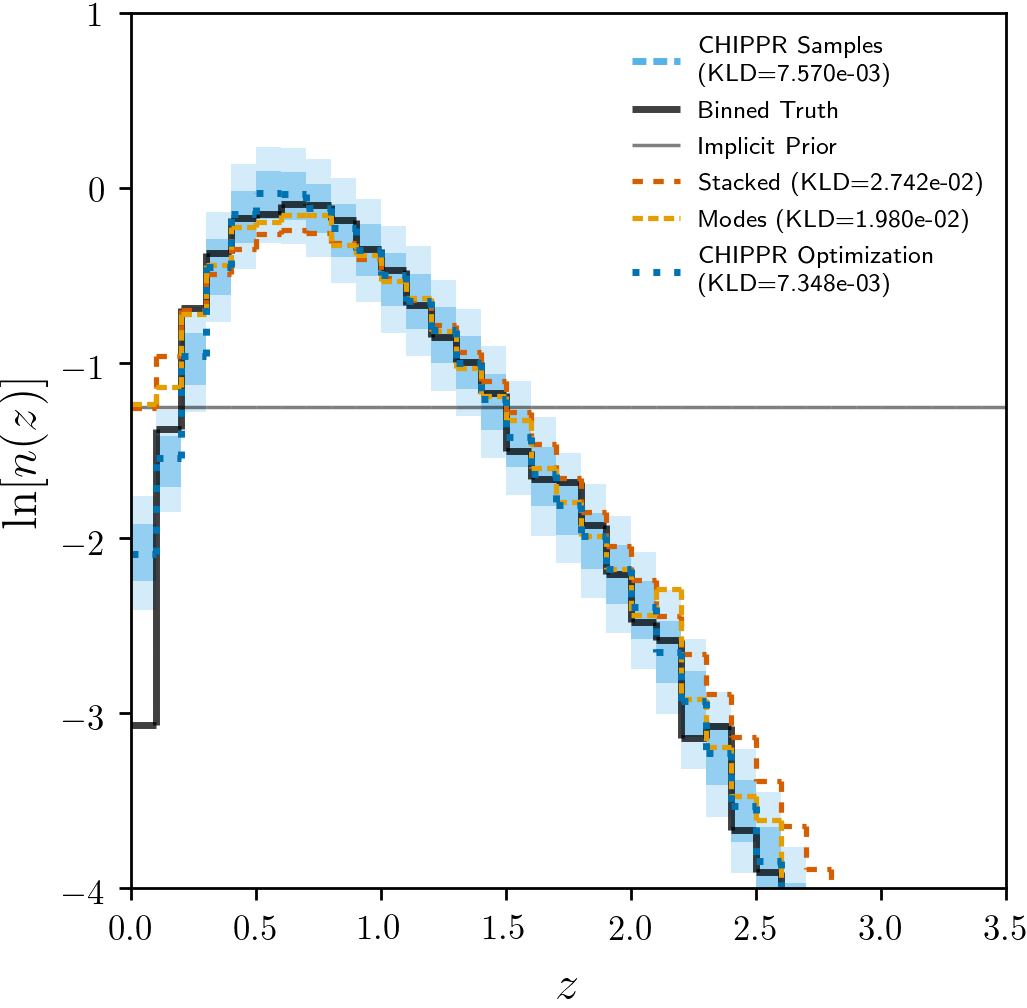
\includegraphics[width=0.45\textwidth]{figures/chippr/results_scatter1.png}
	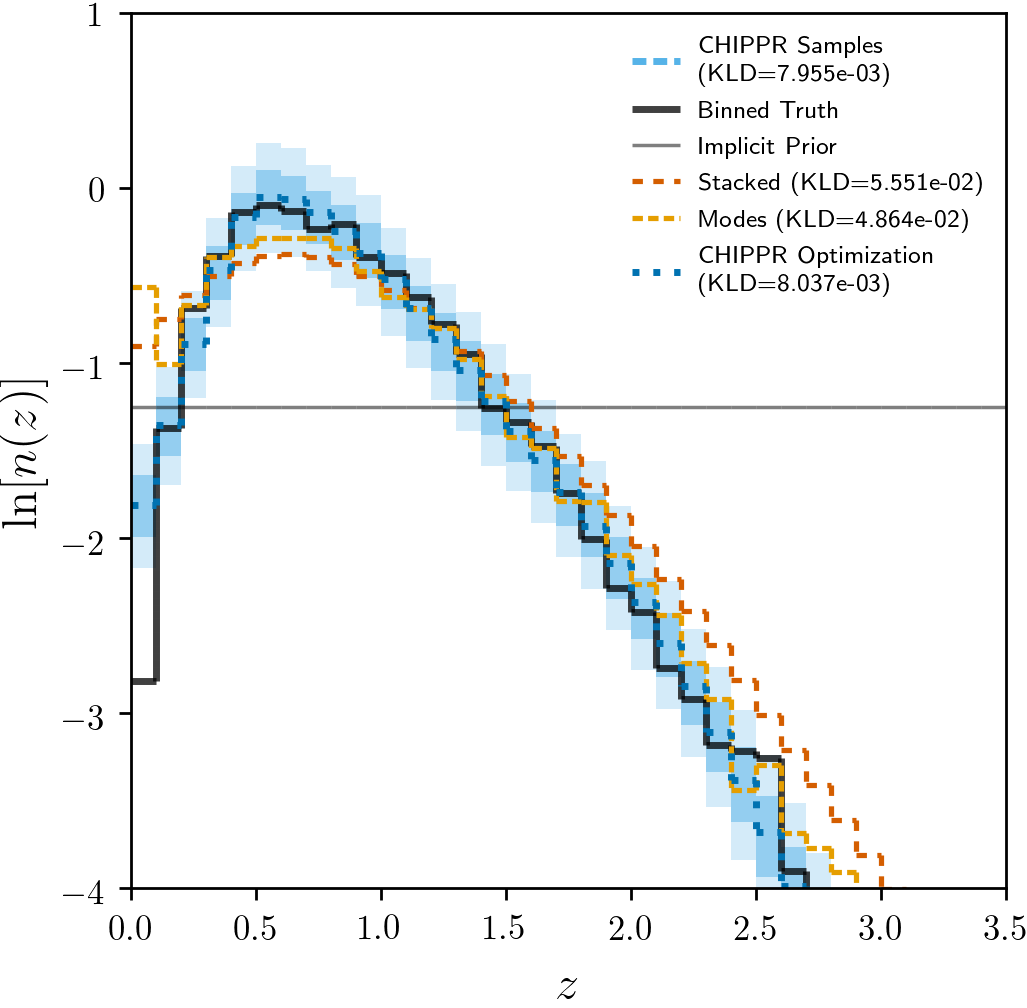
\includegraphics[width=0.45\textwidth]{figures/chippr/results_scatter2.png}
	\caption{
		The results of \Chippr\ (samples in light blue and optimization in dark blue) and the alternative approaches (the stacked estimator in red and the histogram of modes in yellow) on \pzpdf s with intrinsic scatter of the \lsst\ requirements (left) and twice that (right), with the true redshift density (black curve) and implicit prior (gray curve).
		\Chippr\ is robust to intrinsic scatter, but the alternatives suffer from overly broad \nz\ estimates that worsen with increasing intrinsic scatter.
		\aim{TODO: Label panels.
		Add watermark of ``results of inference'' in UL corner, same for ``mock data'' on other kind of plot.}
	}
	\label{fig:results-scatter}
	\end{center}
\end{figure*}

\subsection{Catastrophic outliers}
\label{sec:outliers}

As was covered in \Sect{sec:intro}, catastrophic outliers tend to be distributed non-uniformly across the space of observed and true redshift.
However, the \lsst\ requirements do not specify details for a distribution of outliers to which they were tuned, and it is still instructive to examine the impact of uniform outliers on the inference of \nz, so we begin by addressing uniformly distributed outliers before considering more realistic outlier distributions.

A uniformly distributed population of outliers was simulated by giving every sample in true redshift a $10\%$ chance of having an observed redshift drawn from a uniform distribution rather than the Gaussian about the true redshift.
Though this results in slightly less than the $10\%$ catastrophic outlier rate, it can be done independently of the definition of the standard deviation so was implemented for demonstrative purposes.
\Fig{fig:uniform-outliers} shows examples of \pzpdf s from a uniformly distributed outlier population at the level of the \lsst\ requirements (left) as well as the results of \Chippr\ and other \nz\ estimation methods (right).
The intrinsic scatter of the tests in this section does not increase with redshift as indicated in Table~\ref{tab:lsstsrd}
in order to isolate the effect of outliers, and is instead held at a constant $\sigma_{z} = 0.02$.

\begin{figure}
	\begin{center}
	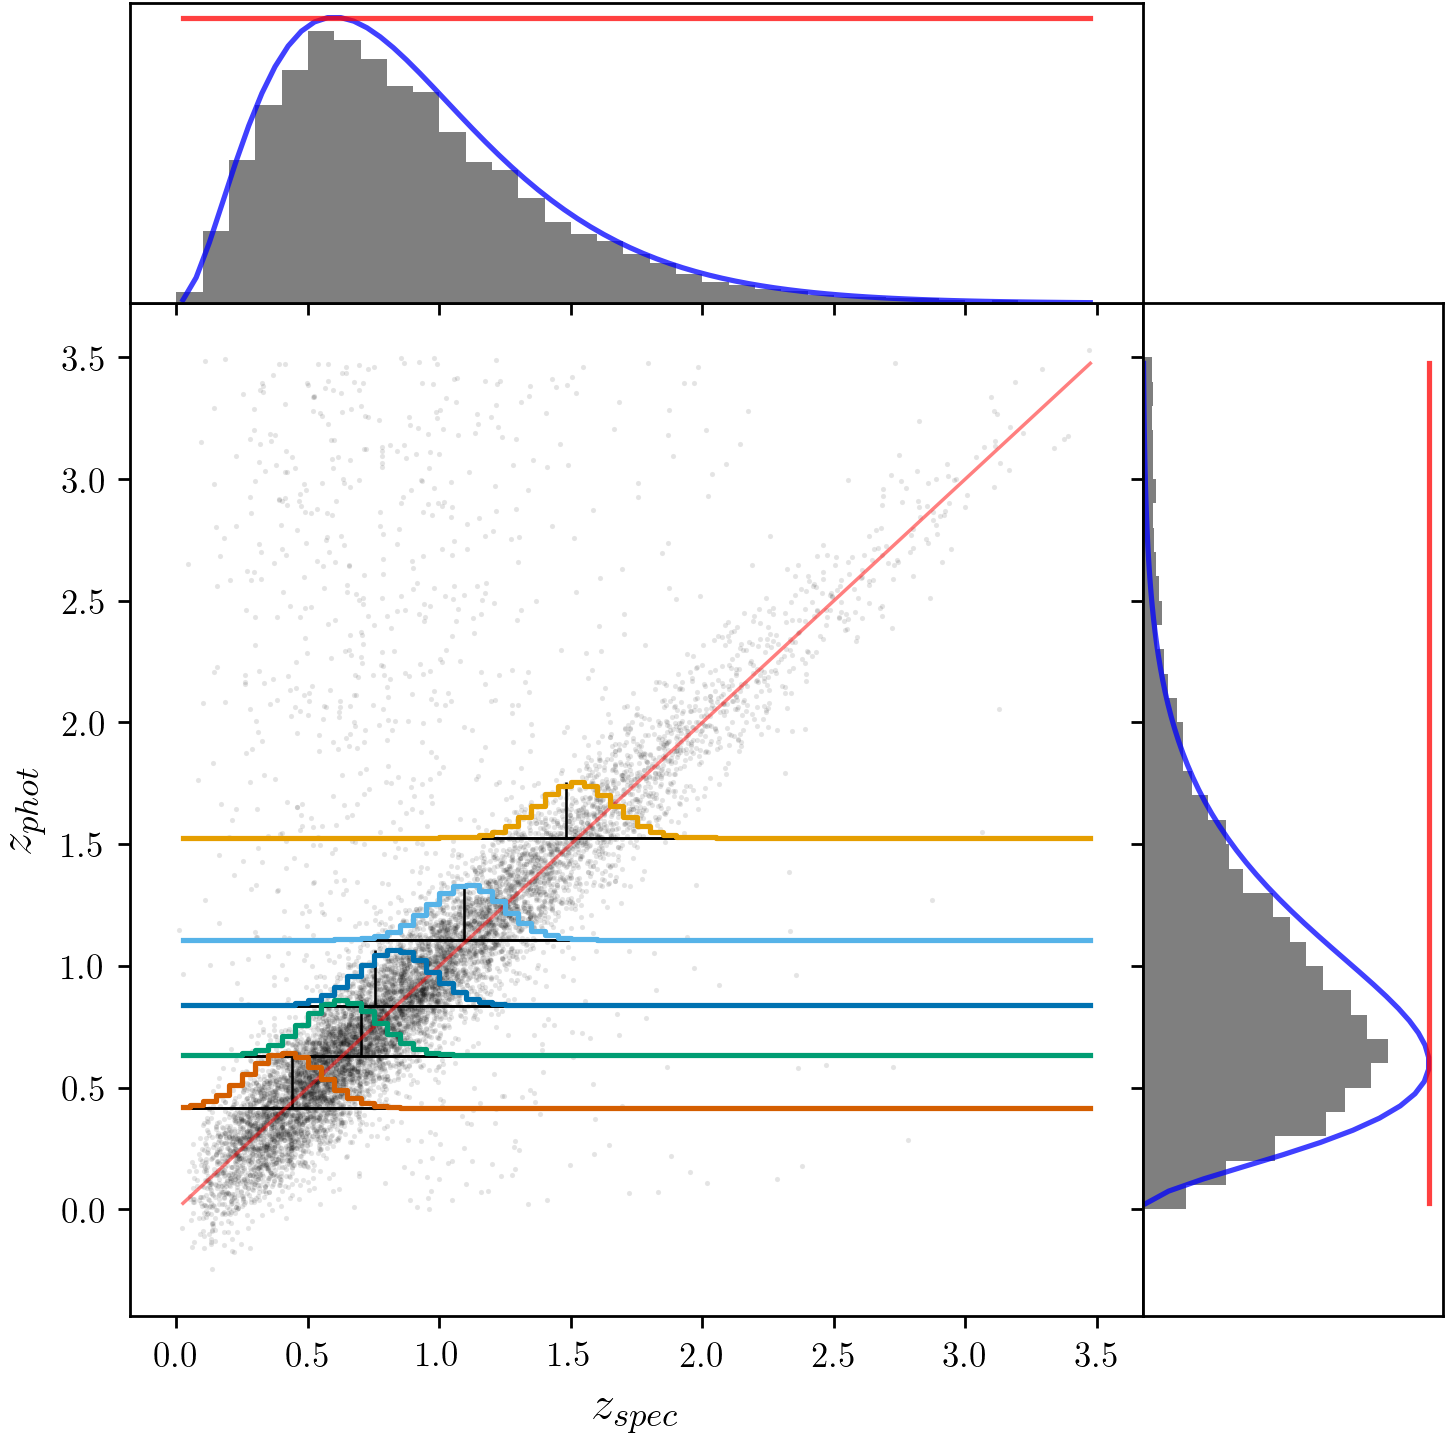
\includegraphics[width=0.45\textwidth]{figures/chippr/single_uout_mega_scatter.png}\\
	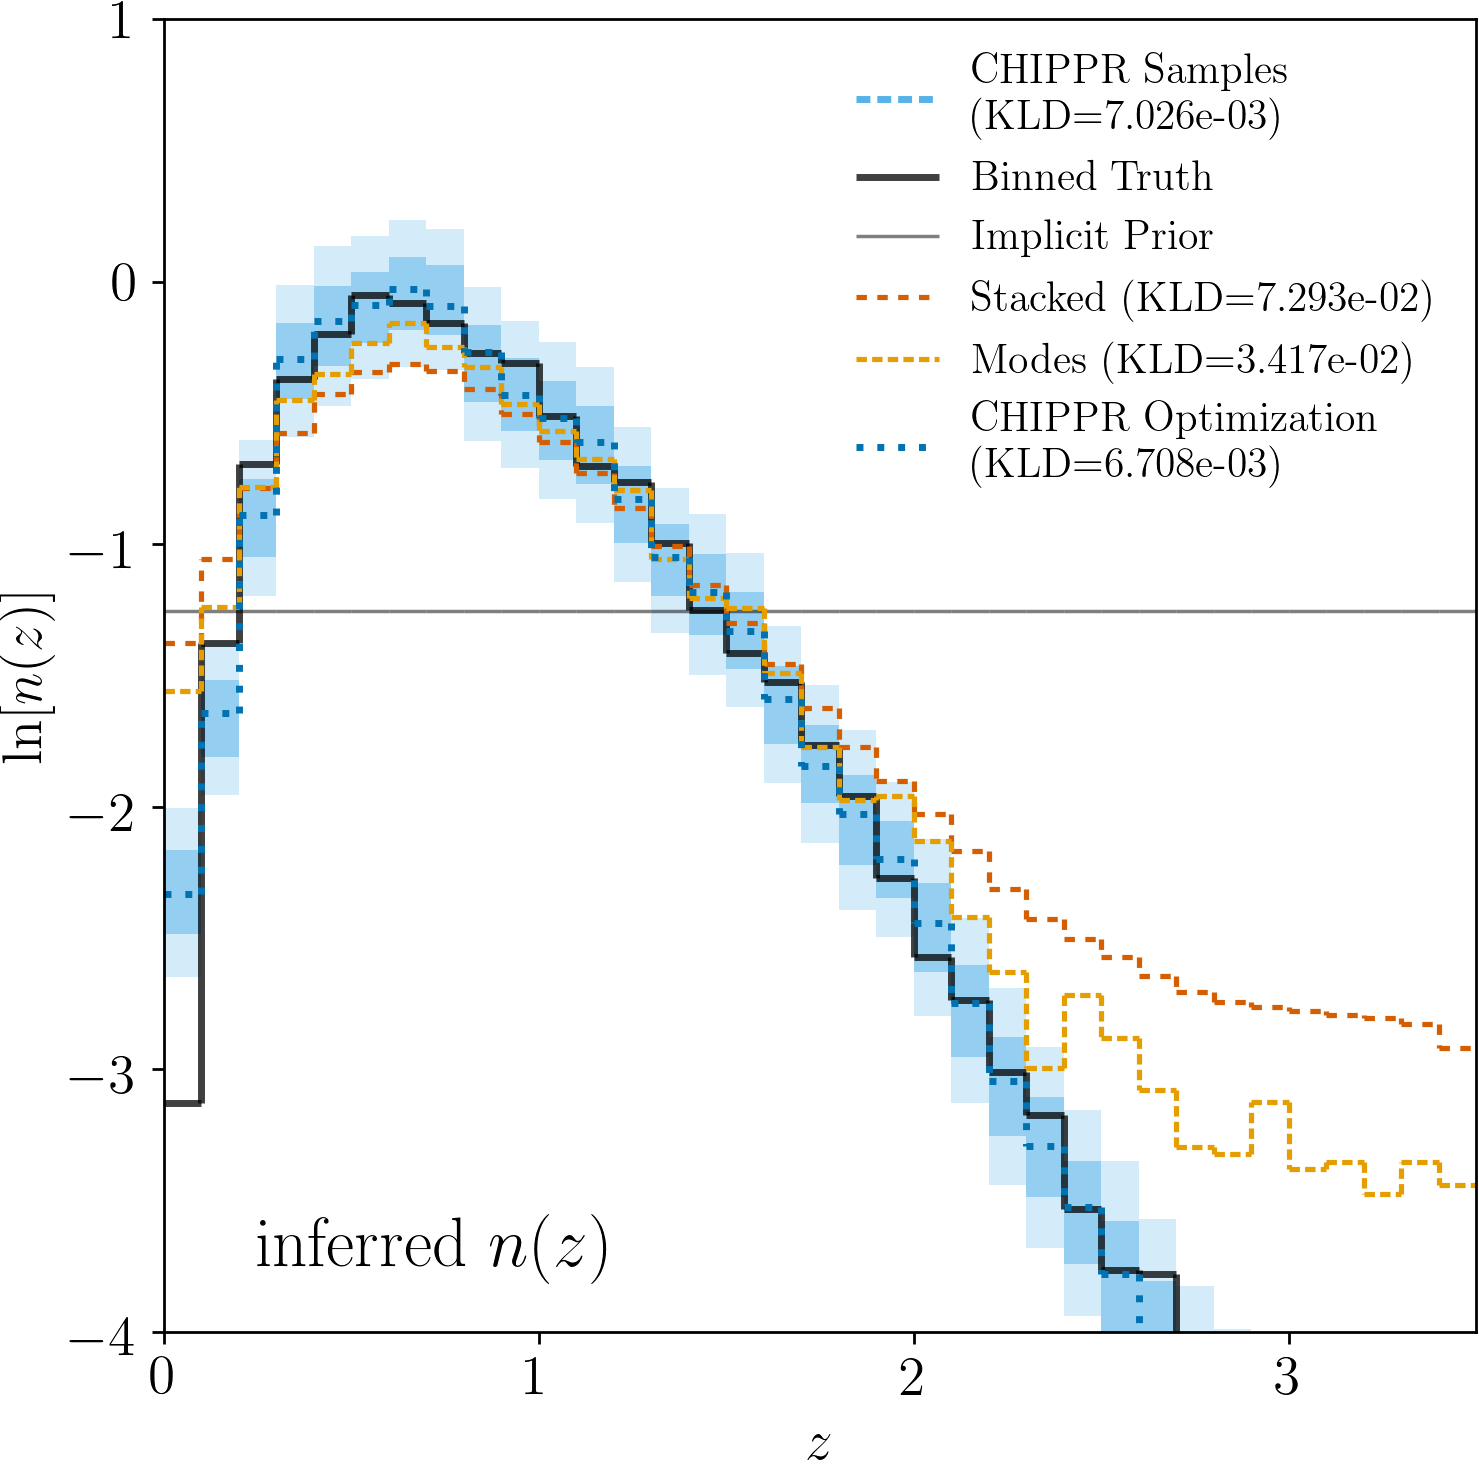
\includegraphics[width=0.45\textwidth]{figures/chippr/single_uout_log_estimators.png}
	\caption{
		Top: Examples of \pzpdf s with a uniform catastrophic outlier population at the level of the \lsst\ requirements, including samples from the probability space of true and observed redshift (black points), \pzpdf s (colored curves), and the true redshifts of the example \pzpdf s (black vertical lines), with marginal histograms (gray) for each dimension with the true redshift distribution (blue curve) and implicit prior (red curve) in the insets.
		Bottom: The results of \Chippr\ (samples in light blue, optimization in dark blue) and the alternative approaches (the stacked estimator in red, the histogram of modes in yellow) on \pzpdf s with uniformly distributed catastrophic outliers, with the true redshift density (black curve) and implicit prior (gray curve).
		The presence of the catastrophic outlier population broadens the histogram of modes and stacked estimator of the redshift distribution, but the result of \Chippr\ is unbiased.
		\aim{TODO: Enlarge axis labels on top and label panels.\\
		Also, add watermark of ``mock data'' in UL corner of top panel and ``results of inference'' on bottom panel.}
	}
	\label{fig:uniform-outliers}
	\end{center}
\end{figure}

\Fig{fig:uniform-outliers} shows that at the level of the \lsst\ requirements, the alternative estimators are overly broad, whereas \Chippr's \mmle\ yields an unbiased estimate of \nz.
Further, the result of stacking is even broader than that of the histogram of modes, corresponding to ten times the information loss of \Chippr's \mmle, making it worse than the most naive reduction of \pzpdf s to point estimates.

When one thinks of the \pzpdf s of catastrophic outliers, however, what comes to mind is multimodal \pzpdf s, wherein reducing \pzpdf s to point estimates to make a standard scatterplot of the true and observed redshifts leads to substantial probability density off the diagonal.
These coordinated catastrophic outliers may be emulated in the joint probability space of true and estimated redshifts by using a mixture of the unbiased diagonal defined by the intrinsic scatter and an additional Gaussian in one dimension, with constant observed redshift for a template-fitting code and constant true redshift for a machine learning code.

In the case of a catastrophic outlier population like that anticipated of template-fitting codes, $10\%$ of all galaxies have their observed redshift at a particular value unrelated to their true redshift, illustrated in the left panel of \Fig{fig:nonuniform-outliers-data}.
This case is subject to the same caveat as the uniformly distributed outliers when it comes to the \lsst\ requirement.
It is less straightforward to emulate catastrophic outliers like those anticipated of a machine learning code, those that are truly multimodal.
The testing conditions here, illustrated in the right panel of \Fig{fig:nonuniform-outliers-data}, gives $10\%$ of galaxies at the redshift affected by outliers an observed redshift that is uniformly distributed relative to the true redshift, meaning that far fewer than $10\%$ of all galaxies in the sample are catastrophic outliers.

\begin{figure*}
	\begin{center}
	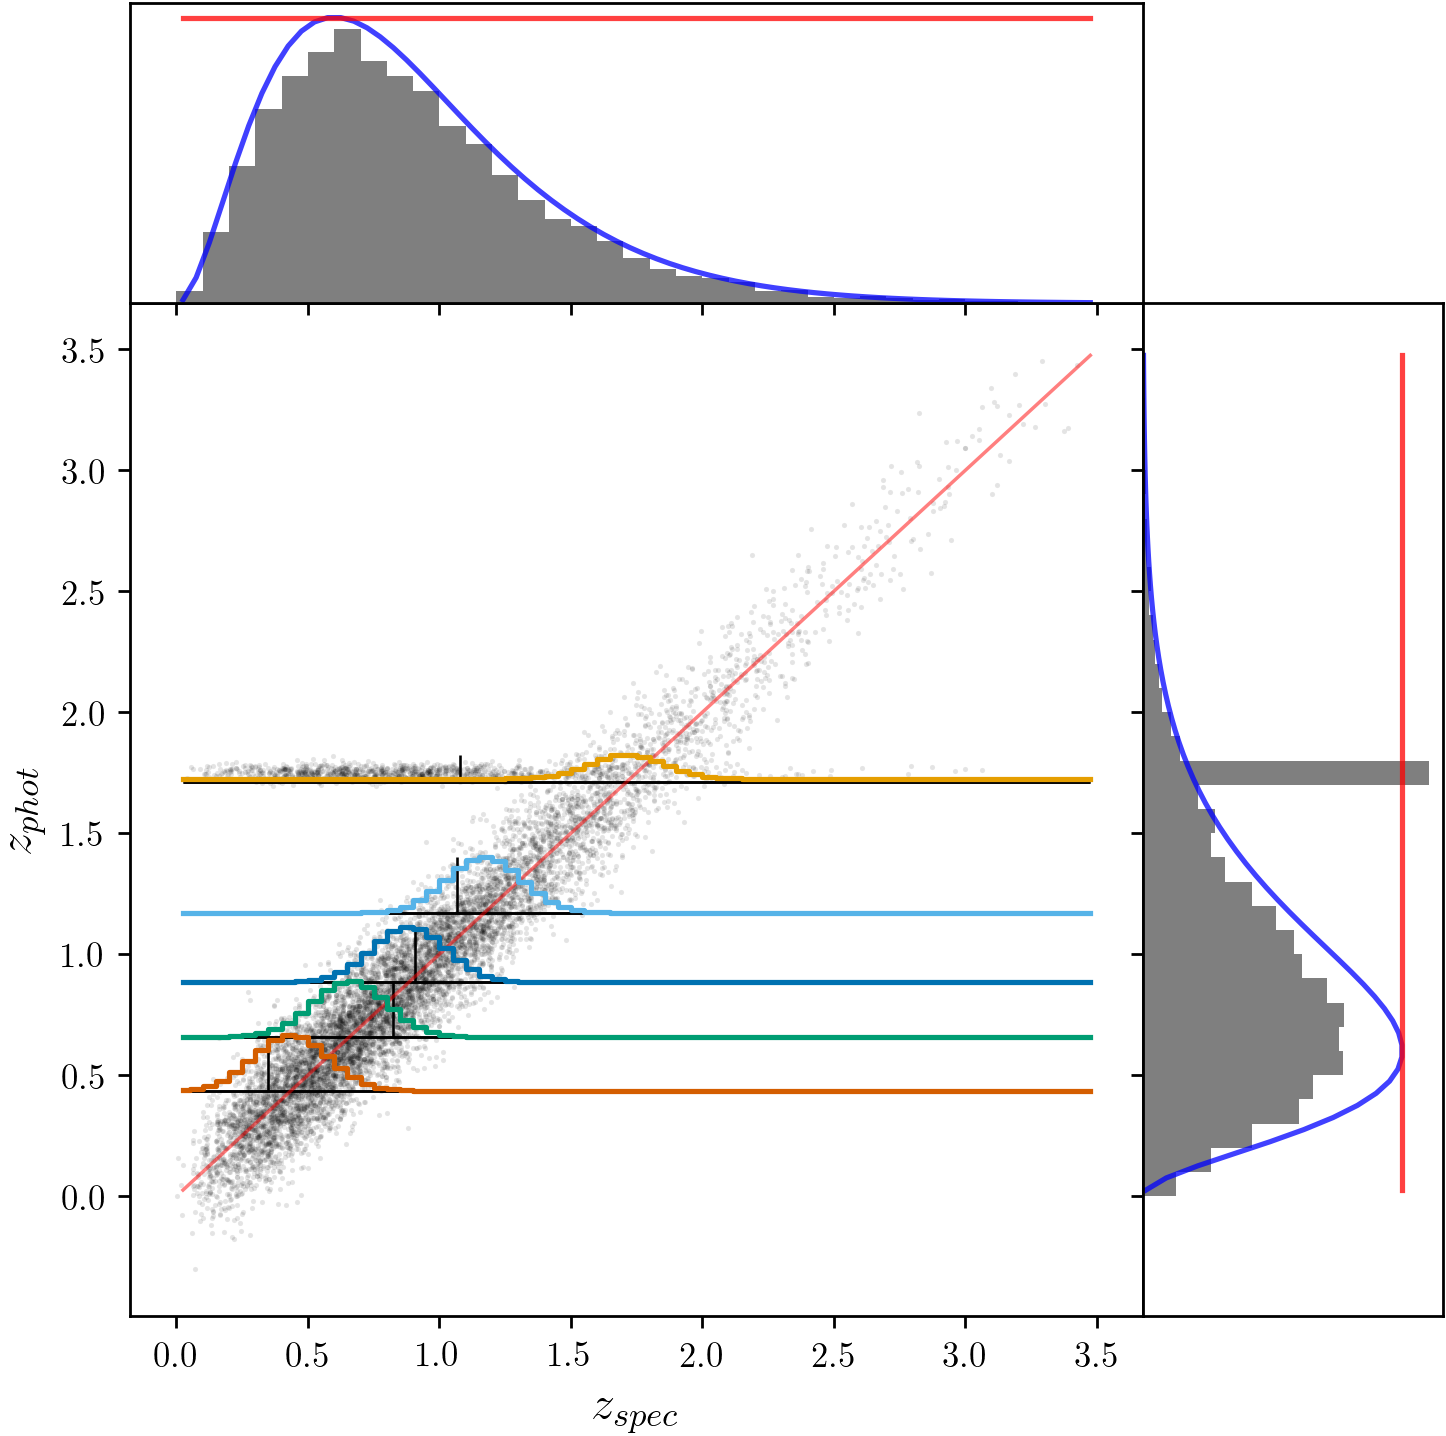
\includegraphics[width=0.45\textwidth]{figures/chippr/thesis_eout_mega_scatter.png}
	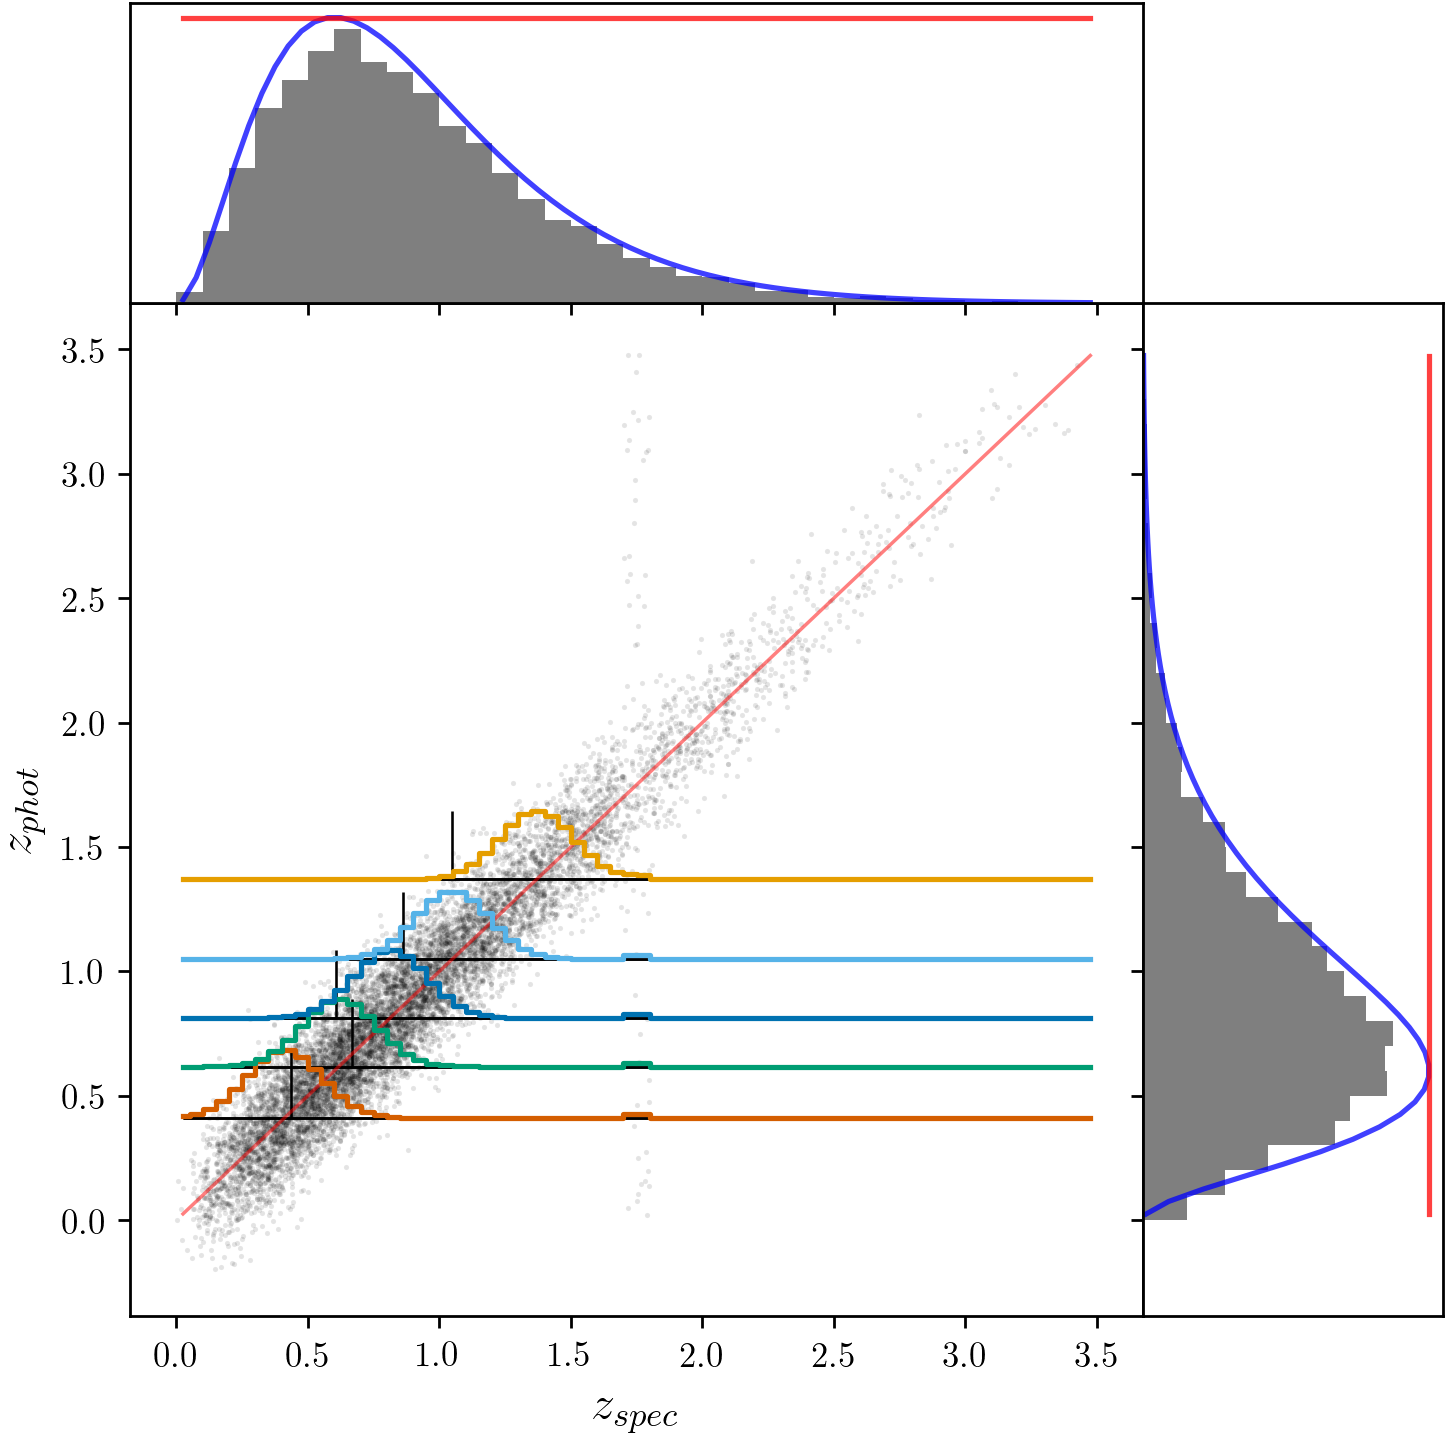
\includegraphics[width=0.45\textwidth]{figures/chippr/thesis_rout_mega_scatter.png}
	\caption{
		Examples of \pzpdf s with a catastrophic outlier population like that seen in template-fitting \pzpdf\ codes (left) and machine learning \pzpdf\ codes (right), including samples from the probability space of true and observed redshift (black points), \pzpdf s (colored curves), and the true redshifts of the example \pzpdf s (black vertical lines), with marginal histograms (gray) for each dimension with the true redshift distribution (blue curve) and implicit prior (red curve) in the insets.
		\aim{TODO: Enlarge axis labels and label panels.
		Add watermark of ``mock data'' in UL corner, same for ``results of inference'' on other kind of plot.}		
	}
	\label{fig:nonuniform-outliers-data}
	\end{center}
\end{figure*}

The results of \Chippr\ and the alternative estimators of \nz\ are presented in \Fig{fig:nonuniform-outliers-results}.
The most striking feature is that the histogram of modes is highly sensitive to both outlier populations, producing a severe overestimate in the case of an outlier population like those seen in template-fitting codes and a severe underestimate in the case of an outlier population like those seen in machine learning codes, corresponding to a twenty-fold loss of information compared to the \Chippr\ \mmle\ in both cases.
The effect on the stacked estimator of \nz\ is more subtle though still concerning.
In the case of outliers like those resulting from template-fitting, the stacked estimator is overly broad even without realistic intrinsic scatter, resulting in ten times the information loss compared to the \Chippr\ \mmle, and in the case of outliers like those resulting from machine learning, the stacked estimator features an overestimate at the redshift affected by the outlier population, resulting in about five times the information loss as the \Chippr\ \mmle.
The \Chippr\ \mmle, however, appears unbiased and withstands these effects, and the breadth of the distribution of samples of \nz\ is invariant.

\begin{figure*}
	\begin{center}
	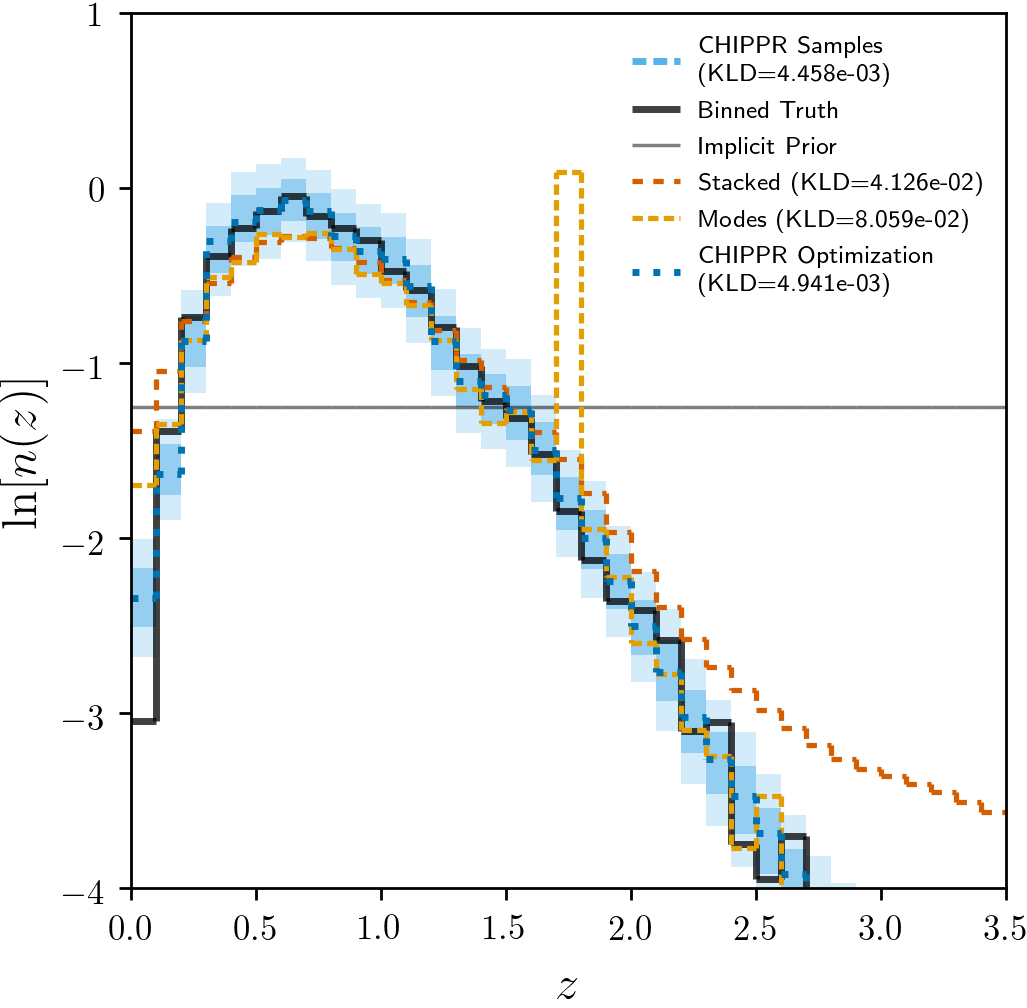
\includegraphics[width=0.45\textwidth]{figures/chippr/thesis_eout_log_estimators.png}
	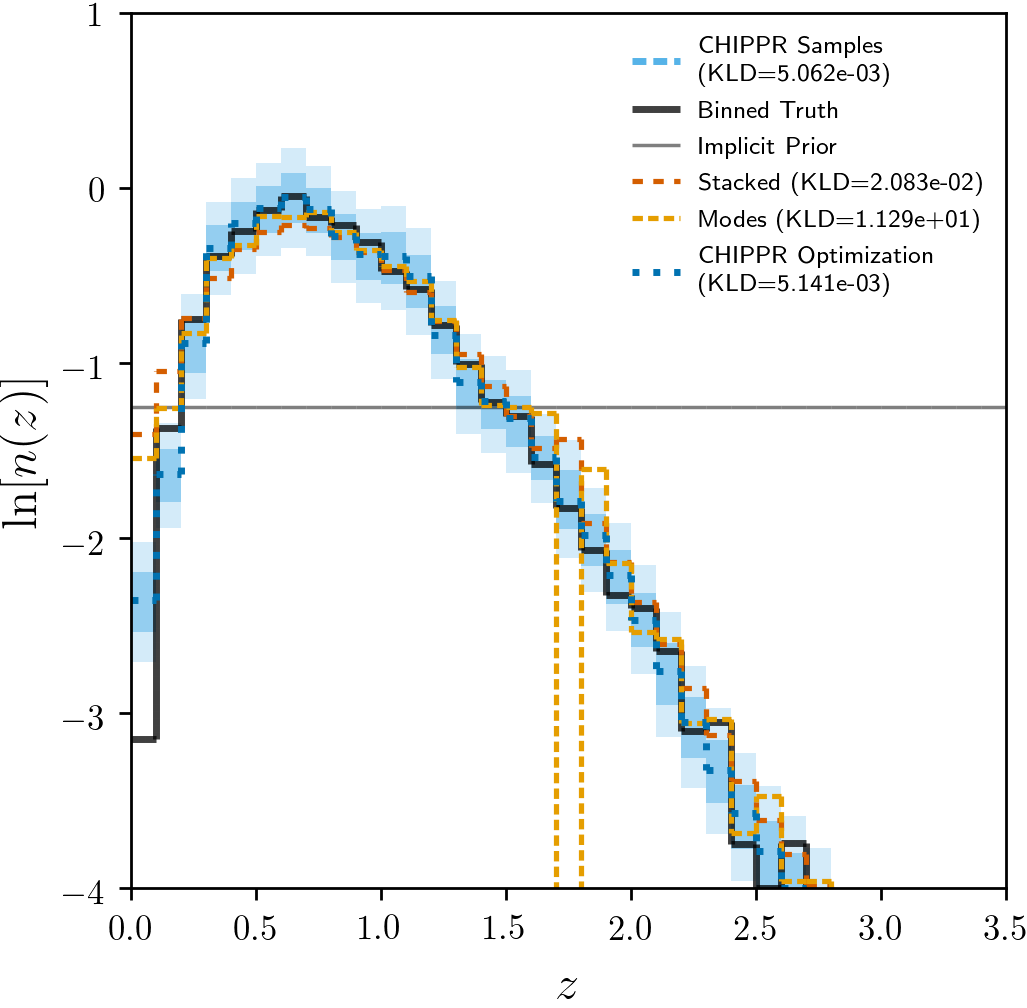
\includegraphics[width=0.45\textwidth]{figures/chippr/thesis_rout_log_estimators.png}
	\caption{
		The results of \Chippr\ (samples in light blue and optimization in dark blue) and the alternative approaches (the stacked estimator in red, the histogram of modes in yellow) on \pzpdf s with catastrophic outliers like those seen in template-fitting \pzpdf\ codes (left) and machine learning \pzpdf\ codes (right) to the \lsst\ requirements, with the true redshift density (black curve) and implicit prior (gray curve).
		Though the histogram of modes is most sensitive to a catastrophic outlier population, the stacked estimator also overestimates \nz\ under (machine learning-like outliers) and beyond (template fitting-like outliers).
		\aim{TODO: Label panels.
		Add watermark of ``results of inference'' in UL corner, same for ``mock data'' on other kind of plot.}
	}
	\label{fig:nonuniform-outliers-results}
	\end{center}
\end{figure*}

\subsection{Systematic bias}
\label{sec:bias}

Systematic bias in \pz\ point estimates is a concern for \lsst's cosmology results, for the same reasons explored in \citet{hoyle_dark_2017}.
However, in the context of \pzpdf s, the notion of redshift bias is a form of model misspecification.
Consider that if bias were included in the framework of Figure~\ref{fig:pedagogical_scatter};
a simple linear transformation of $z_{\mathrm{phot}} \to z_{\mathrm{phot}} - \Delta_{z} (1 + z_{\mathrm{phot}})$ would eliminate the bias.
Regardless, for completeness, a test at ten times the bias of the \lsst\ requirements, with no redshift-dependent intrinsic scatter nor catastrophic outliers, is provided in \Fig{fig:bias}.

\begin{figure}
	\begin{center}
	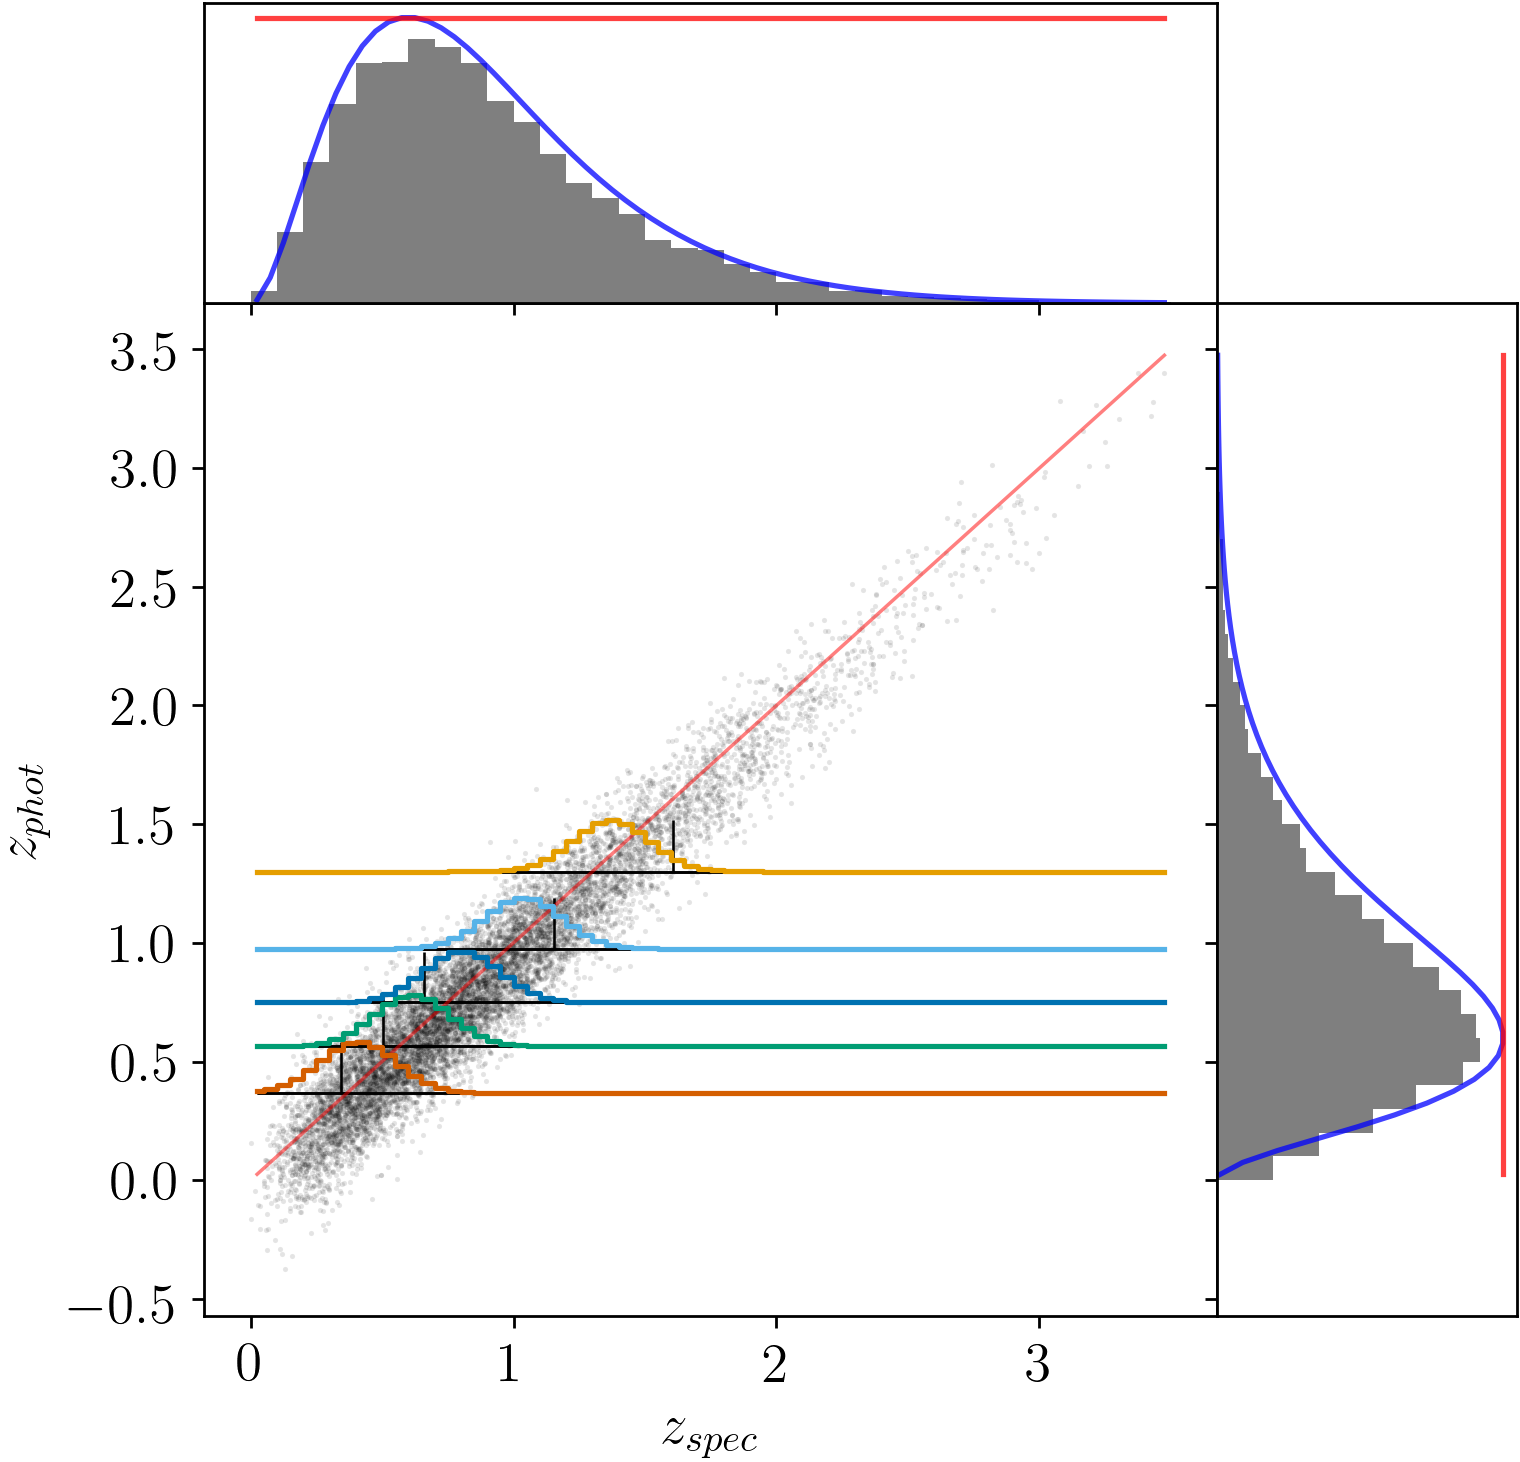
\includegraphics[width=0.45\textwidth]{figures/chippr/thesis_neghivarbias_mega_scatter.png}\\
	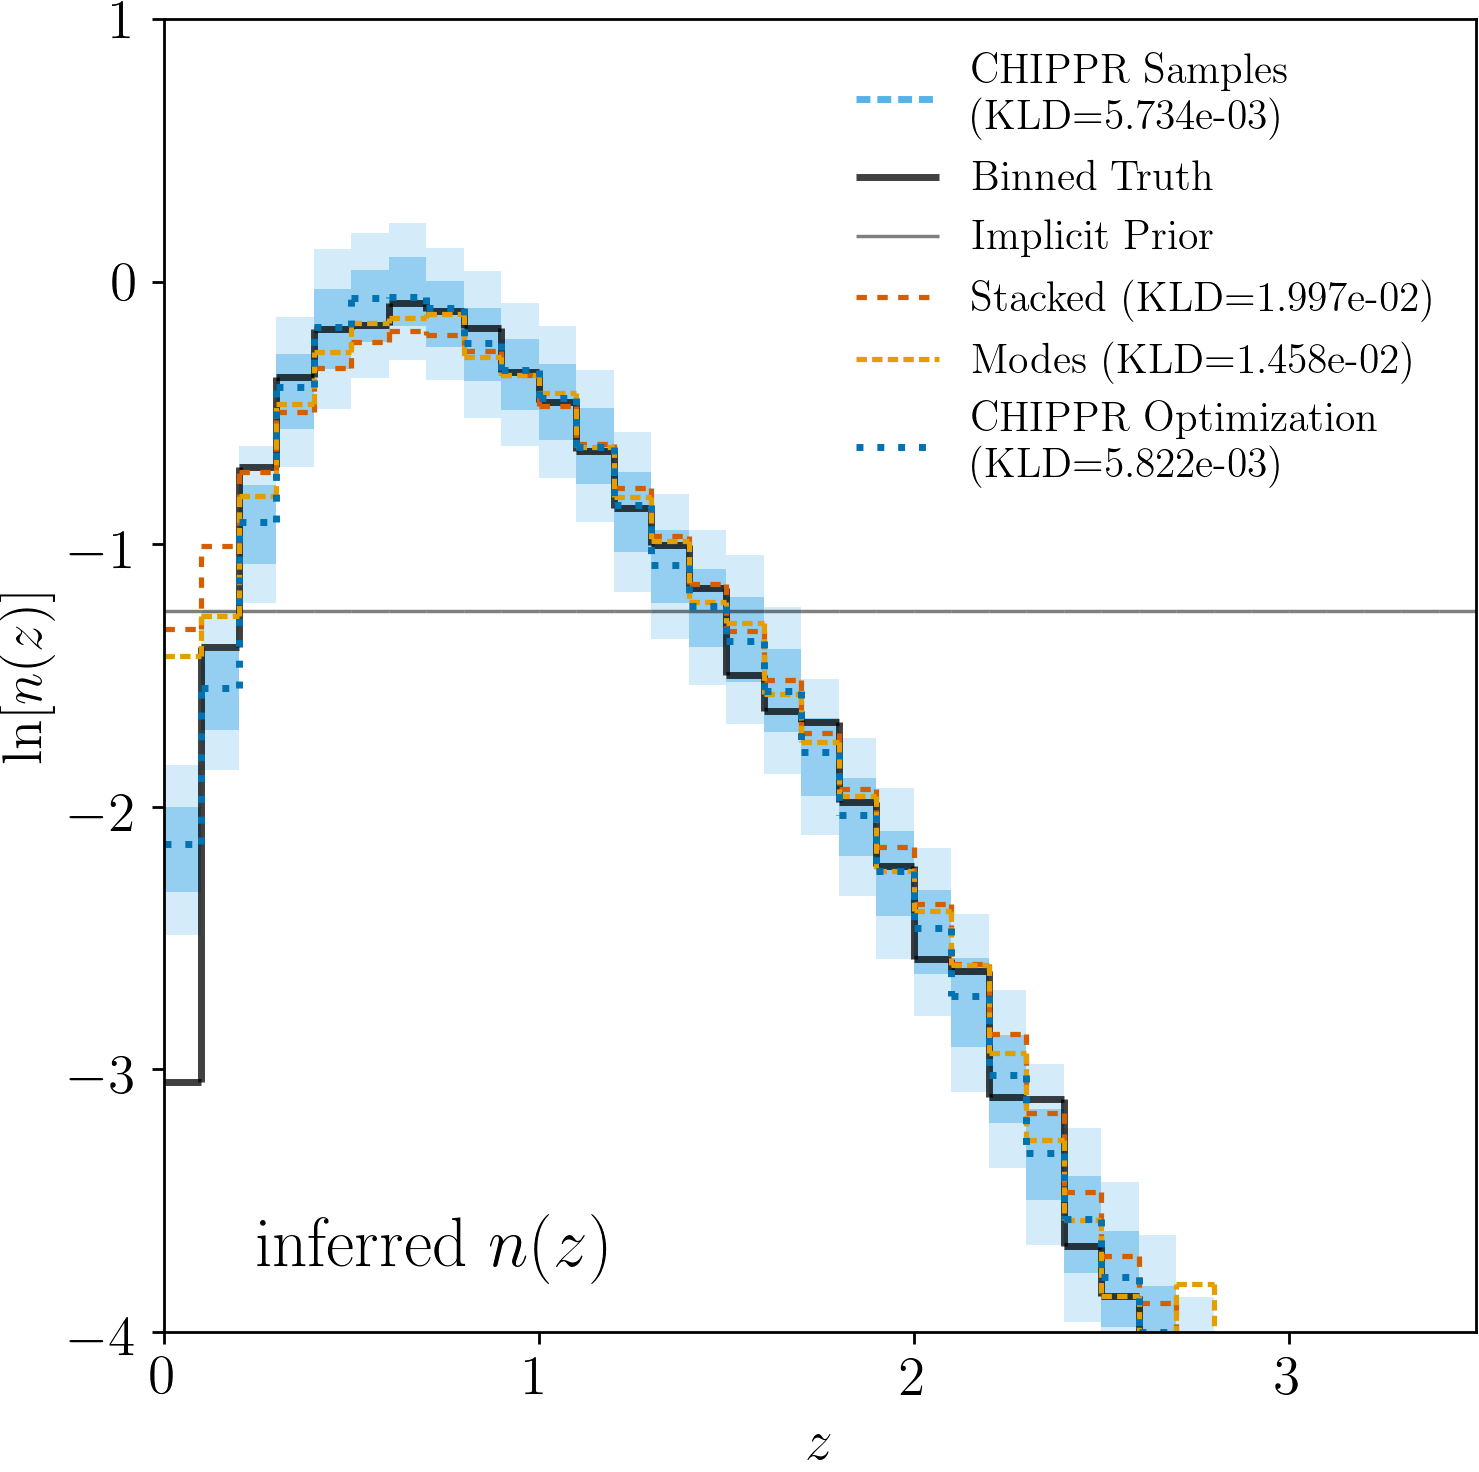
\includegraphics[width=0.45\textwidth]{figures/chippr/thesis_neghivarbias_log_estimators.png}
	\caption{
		Left: Examples of \pzpdf s with ten times the bias of the \lsst\ requirements, including samples from the probability space of true and observed redshift (black points), \pzpdf s (colored curves), and the true redshifts of the example \pzpdf s (black vertical lines), with marginal histograms (gray) for each dimension with the true redshift distribution (blue curve) and implicit prior (red curve) in the insets.
		Right: The results of \Chippr\ (samples in light blue, optimization in dark blue) and the alternative approaches (the stacked estimator in red, the histogram of modes in yellow) on \pzpdf s with uniformly distributed catastrophic outliers, with the true redshift density (black curve) and implicit prior (gray curve).
		The impact of bias at even ten times the level of the \lsst\ requirements is almost imperceptible on all estimators, though the \Chippr\ \mmle\ minimizes the information loss regardless.
		\aim{TODO: Enlarge axis labels on top and label panels.
		Also, add watermark of ``mock data'' in UL corner of top panel and ``results of inference'' on bottom panel.}
	}
	\label{fig:bias}
	\end{center}
\end{figure}

As expected based on consistency with the forward model, \Chippr\ is completely resistant to bias, and the alternative estimators are only weakly affected, with information loss two and four times greater than that of the \Chippr\ \mmle\ for the histogram of modes and stacked estimator respectively.
\que{Did I effectively explain why \Chippr\ is expected to be unaffected by bias of this form?}

\subsection{Implicit prior}
\label{sec:interim}

\chippr\ can handle any implicit prior with support over the redshift range where \nz\ is defined, but some archetypes of implicit prior are more likely to be encountered in the wilds of \pzpdf\ codes.
Ideally, an uninformative implicit prior would be used, although it may be complicated to compute from the covariances of the raw data.  
Template-fitting codes have an explicit prior input formed by redshifting a small number of templates, leading to a highly nonuniform but physically-motivated interim prior.
%Another potential method for selecting an interim prior with support over the entire redshift range expected of the photometric survey is to sum two or more $N(z)$ distributions obtained from reliable photometric surveys in the past.  
%This is just as problematic as using a biased spectroscopically derived $N(z)$ as the interim prior because the sum of redshift distributions for two or more surveys does not reflect our beliefs about the true distribution for a single survey even though it provides support over the same redshift range.  
%To simulate this case, we choose an interim prior with more weight at high and low redshifts than for mid-range redshifts.  
Machine learning approaches tend to be trained on previously observed data sets that are biased towards low redshift, which biases the implicit prior towards low redshift.
% \aim{reference chapter 3 for complication of algorithm}
Some efforts have been made to modify an observationally informed implicit prior so that it is more representative of the photometric data for which redshifts are desired \citep{sheldon_photometric_2012}, but, unless it is equal to the true \nz, it will propagate to the results of traditional \nz\ estimation methods.  
%Because low-redshift galaxies are more likely to be bright enough to be observed by such a survey, $N(z)$ determined from that sample may be heavily biased to low redshift galaxies.  
%By contrast, the galaxies that were unobserved in such a survey are more likely be dimmer, making them more likely to be at higher redshifts.  
%Since the interim prior is not compatible with our beliefs about the true redshift distribution, the resulting interim redshift posteriors will be inappropriate.  

\Fig{fig:pzs-priors} shows examples of \pzpdf s with a low-redshift favoring implicit prior emulating that of a machine learning approach to \pz\ estimation (left panel) and a more complex interim prior emulating that of a template-fitting \pz\ method (right panel).
One can see that the \pzpdf s take different shapes from one another even though the marginal histograms of the points are identical.
The machine learning-like implicit prior has been modified to have nonzero value at high-redshift because the implicit prior must be strictly positive definite for the \Chippr\ model to be valid.

\begin{figure*}
	\begin{center}
	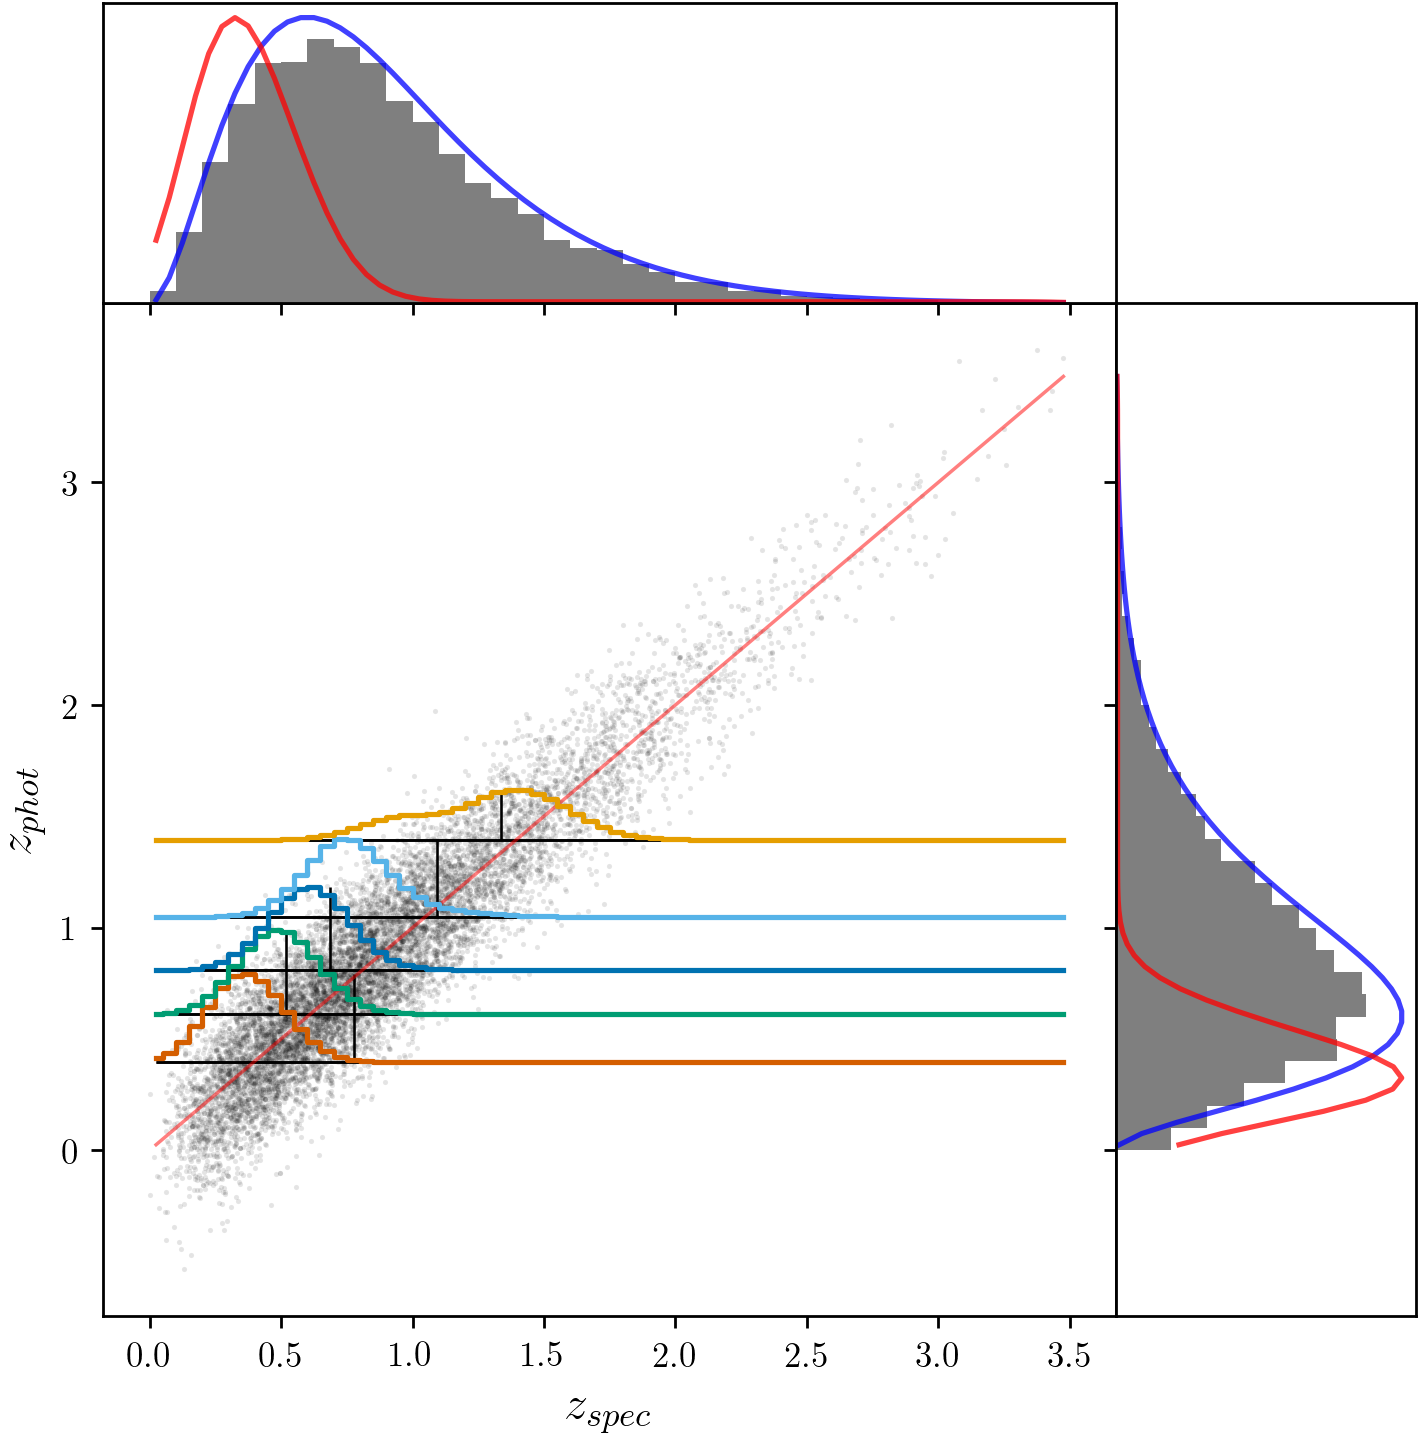
\includegraphics[width=0.45\textwidth]{figures/chippr/samplepzs_trpr.png}
	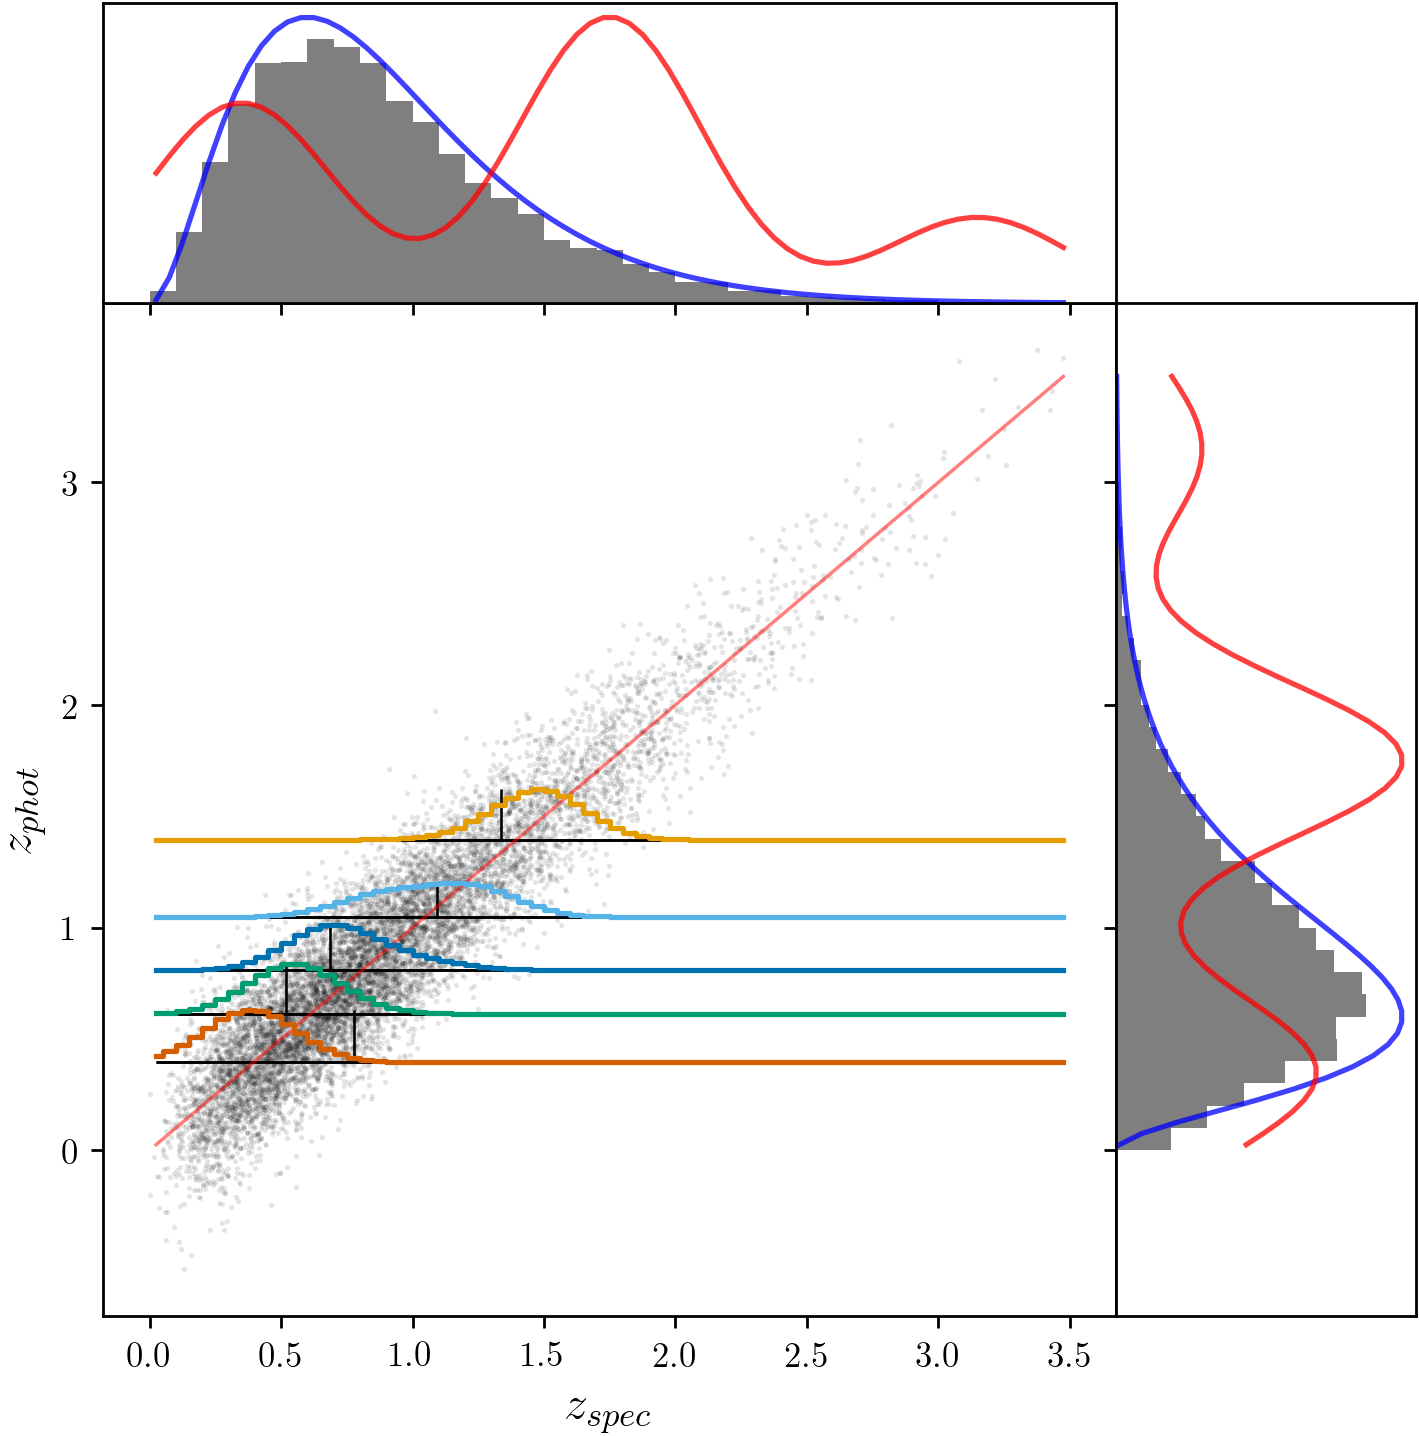
\includegraphics[width=0.45\textwidth]{figures/chippr/samplepzs_tmpr.png}
	\caption{
		Examples of mock \pzpdf s (colored lines) generated with a machine learning-like implicit prior (left) and a template-fitting-like implicit prior (right), including samples from the probability space of true and observed redshift (black points), \pzpdf s (colored lines), the true redshifts of the example \pzpdf s (black vertical lines).
		A histogram (gray) of points in each dimension is shown in the respective inset, with the true redshift distribution (blue curve) and implicit prior (red curve).
		\aim{TODO: Enlarge axis labels.
		Label panels.
		Add watermark of ``mock data'' in UL corner, same for ``results of inference'' on other kind of plot.}
	}
	\label{fig:pzs-priors}
	\end{center}
\end{figure*}

\Fig{fig:results-priors} shows the performance of \Chippr\ and the traditional methods on \pzpdf s generated with nontrivial implicit priors.
In both cases, the \Chippr\ \mmle\ effectively recovers the true redshift distribution, and the distribution of \nz\ parameter values reflects higher uncertainty where the implicit prior undergoes large changes in derivative.
The alternatives, on the other hand, are biased by the implicit prior except where it is flat, in the case of high redshifts for the machine learning-like implicit prior, resulting in over $1,000$ times the information loss on \nz\ for the machine learning-like implicit prior and some $5-20$ times the information loss for the template fitting-like implicit prior, relative to the \Chippr\ \mmle.

\begin{figure*}
	\begin{center}
	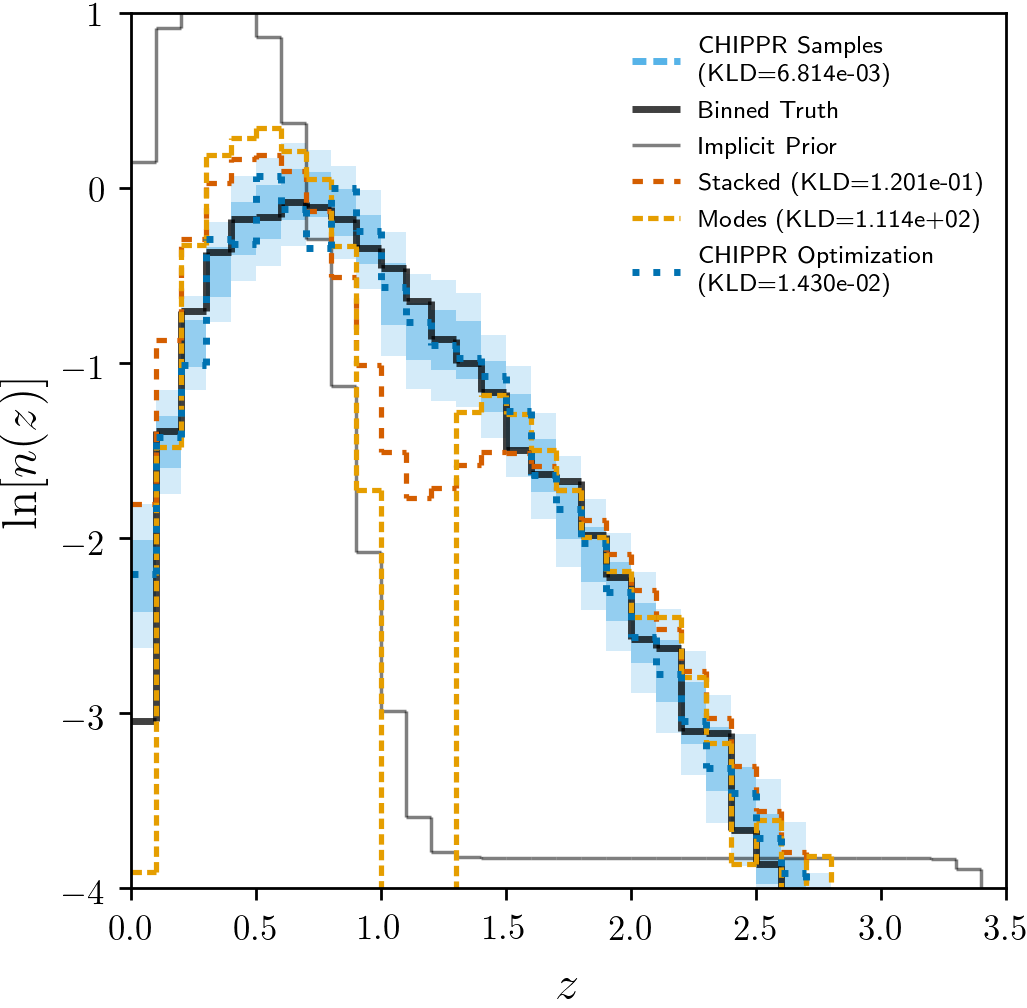
\includegraphics[width=0.45\textwidth]{figures/chippr/results_trpr.png}
	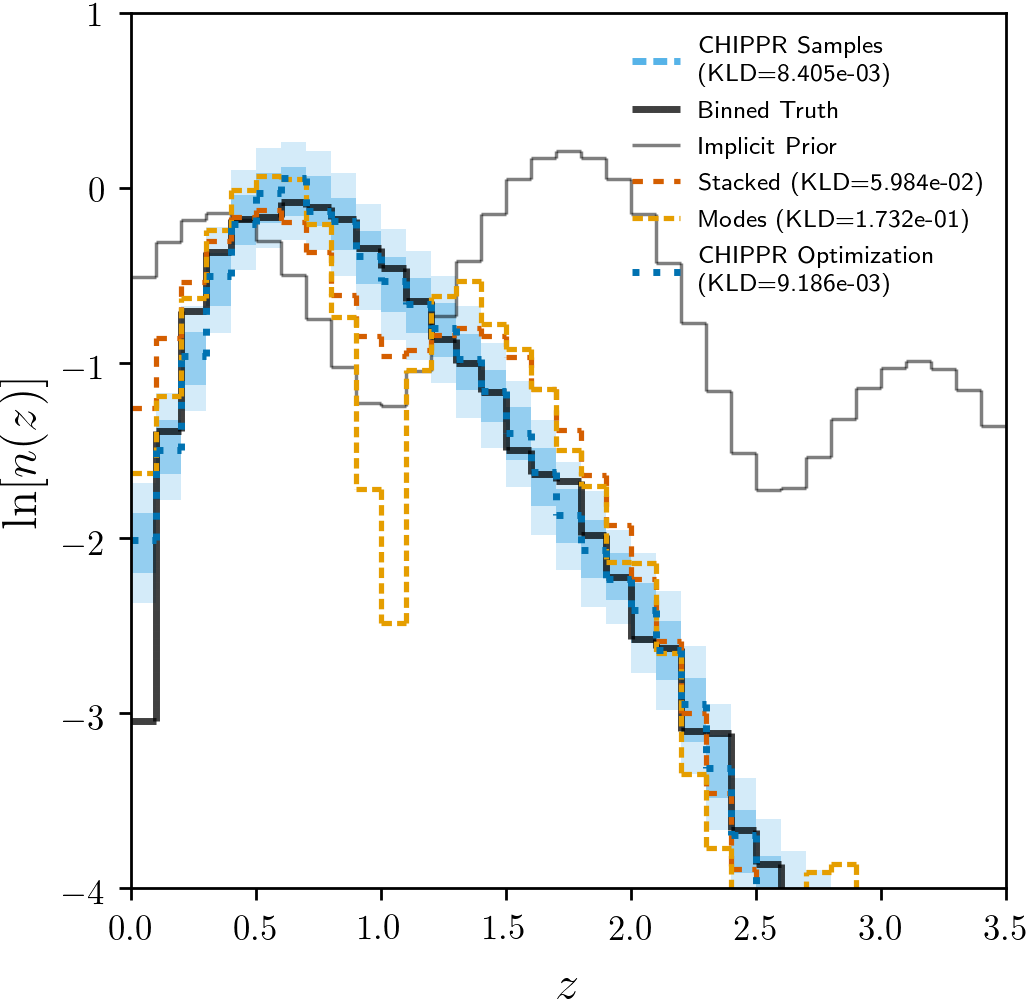
\includegraphics[width=0.45\textwidth]{figures/chippr/results_tmpr.png}
	\caption{
		The results of \Chippr\ (samples in light blue and optimization in dark blue) and the alternative approaches (the stacked estimator in red and the histogram of modes in yellow) on \pzpdf s with an implicit prior like that of machine learning \pzpdf\ approaches (left) and an implicit prior like that of template-fitting \pzpdf\ codes (right), with the true redshift density (black curve) and implicit prior (gray curve).
		\Chippr\ is robust to a nontrivial implicit prior, but the alternatives are biased toward the implicit prior.
		\aim{TODO: Label panels.
		Add watermark of ``results of inference'' in UL corner, same for ``mock data'' on other kind of plot.}
	}
	\label{fig:results-priors}
	\end{center}
\end{figure*}

\que{Move \Sect{sec:violations} here?}

The main implication of the response of \nz\ estimates to a nontrivial implicit prior is that the implicit prior must be accounted for when using \pzpdf\ catalogs.

\section{Discussion}
\label{sec:results}

The experiments of \Sect{sec:alldata} isolate the potential sources of error in \nz\ estimation one at a time.
Now, we stress-test \Chippr\ by investigating two realistically complex cases, one in which the \nz\ estimates are made tomographically as in a modern cosmological analysis (\Sect{sec:lsstdemo}) and one in which the \nz\ estimators are not provided with the same implicit prior used to generate the \pzpdf\ catalog (\Sect{sec:violations}).

\subsection{LSST Requirements}
\label{sec:lsstdemo}

It is of interest to explore the impact of incorrectly estimated \nz\ on the cosmological inference to answer the question of how wrong we will be in our understanding of the universe if we incorrectly constrain \nz.
To test the impact of these uncertainties, we simulate mock data with all three effects with which \lsst\ is concerned at the levels of Table~\ref{tab:lsstsrd} and propagate the results of \Chippr\ and the other estimators to a Fisher matrix forecast using \cosmolike\ \citep{krause_cosmolike_2017}, a publicly available cosmological forecasting code.
%Though redshift tomography is non-physical, as redshift is a continuous random variable, and binning in estimated redshift introduces poorly understood systematic error, we perform this analysis as an example of how it affects the current standard in how cosmological parameters are constrained by galaxy surveys, rather than how we think they ought to be constrained.
%\aim{Don't introduce anti-tomography rant here, kind of controversial and should be explored where it has its own space.}

\begin{figure}
	\begin{center}
		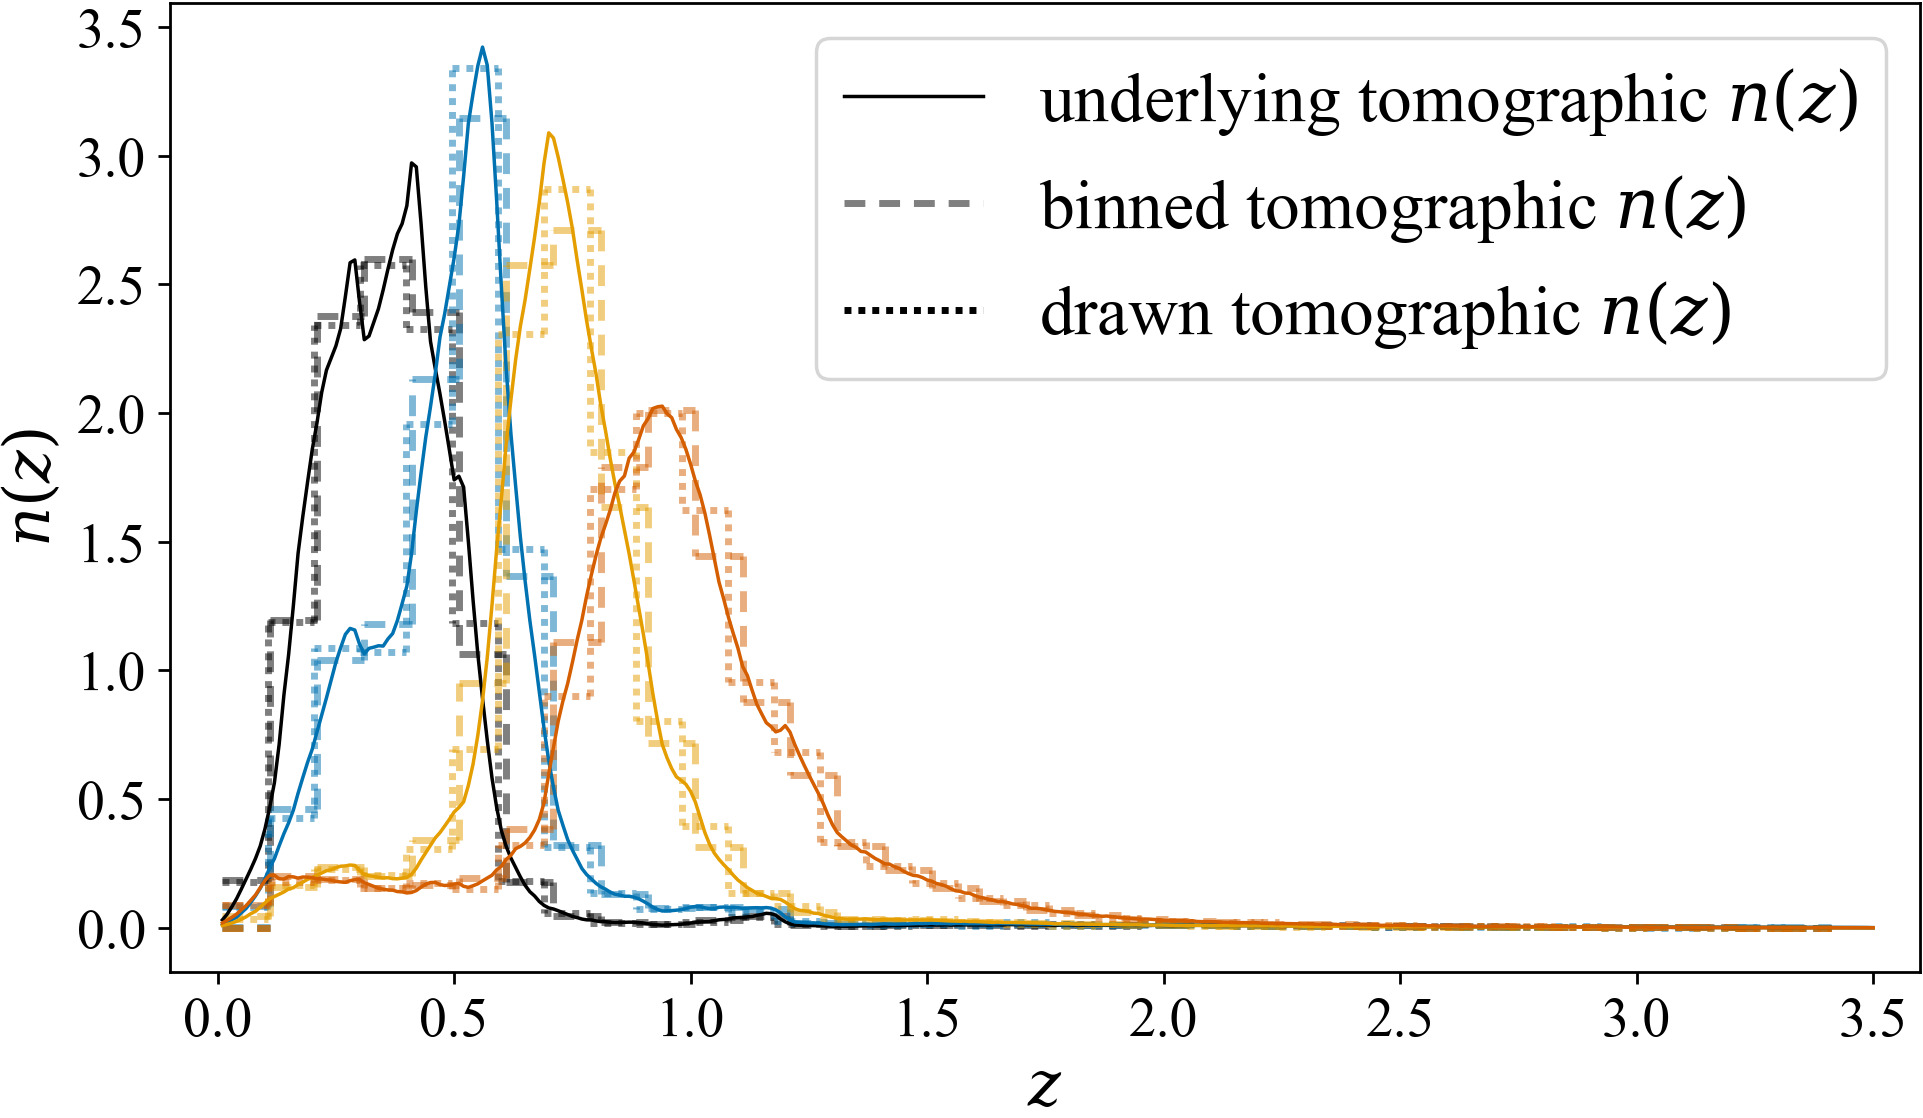
\includegraphics[width=0.45\textwidth]{figures/chippr/cosmolike_inputs.png}
		\caption{
			The \lsst-like tomographic binning and true redshift distribution, where the truth (solid) is a PDF evaluated on a fine grid of $350$ redshifts $0.0101 < z < 3.5001$, and the binned (dashed) and drawn (dotted) \nz\ are piecewise constant functions evaluated in $35$ evenly spaced bins, for four different tomographic bins (colors).
		}
		\label{fig:tomobins}
	\end{center}
\end{figure}

\dwh{We consider as ground truth a set of known \nz\ corresponding to each of four hypothetical samples of galaxies and the corresponding cosmological parameter covariance matrix.
The \nz\ of each galaxy subsample emulates that anticipated of galaxies binned by a redshift point estimate, as is common in tomographic redshift analyses, though our experimental procedure is agnostic to how the samples are identified.
The cosmological parameter covariance matrices are those used for \desc\ forecasting with the ground truth \nz\ in the same four bins.}
The true \nz\ in each pre-defined bin is already provided in the form of an evaluation of a function on a fine grid of $350$ redshifts $0.0101 < z < 3.5001$.

First, we bin them down to a piecewise constant parameterization with a manageable $35$ hyperparameters for \chippr's sampling capabilities.
Next, we draw $10^{4}$ true redshifts from the binned true \nz\ for each tomographic bin.
The original, binned, and drawn \nz\ are shown in \Fig{fig:tomobins}.
We emulate \pzpdf s for the $10^{4}$ true redshifts drawn from the true \nz\ in each bin using the procedure of \Fig{fig:flowchart} with all three effects of Table~\ref{tab:lsstsrd}
at their given levels.
Illustrations of this process are provided in \Fig{fig:per-bin-scatter}.

\begin{figure*}
	\begin{center}
		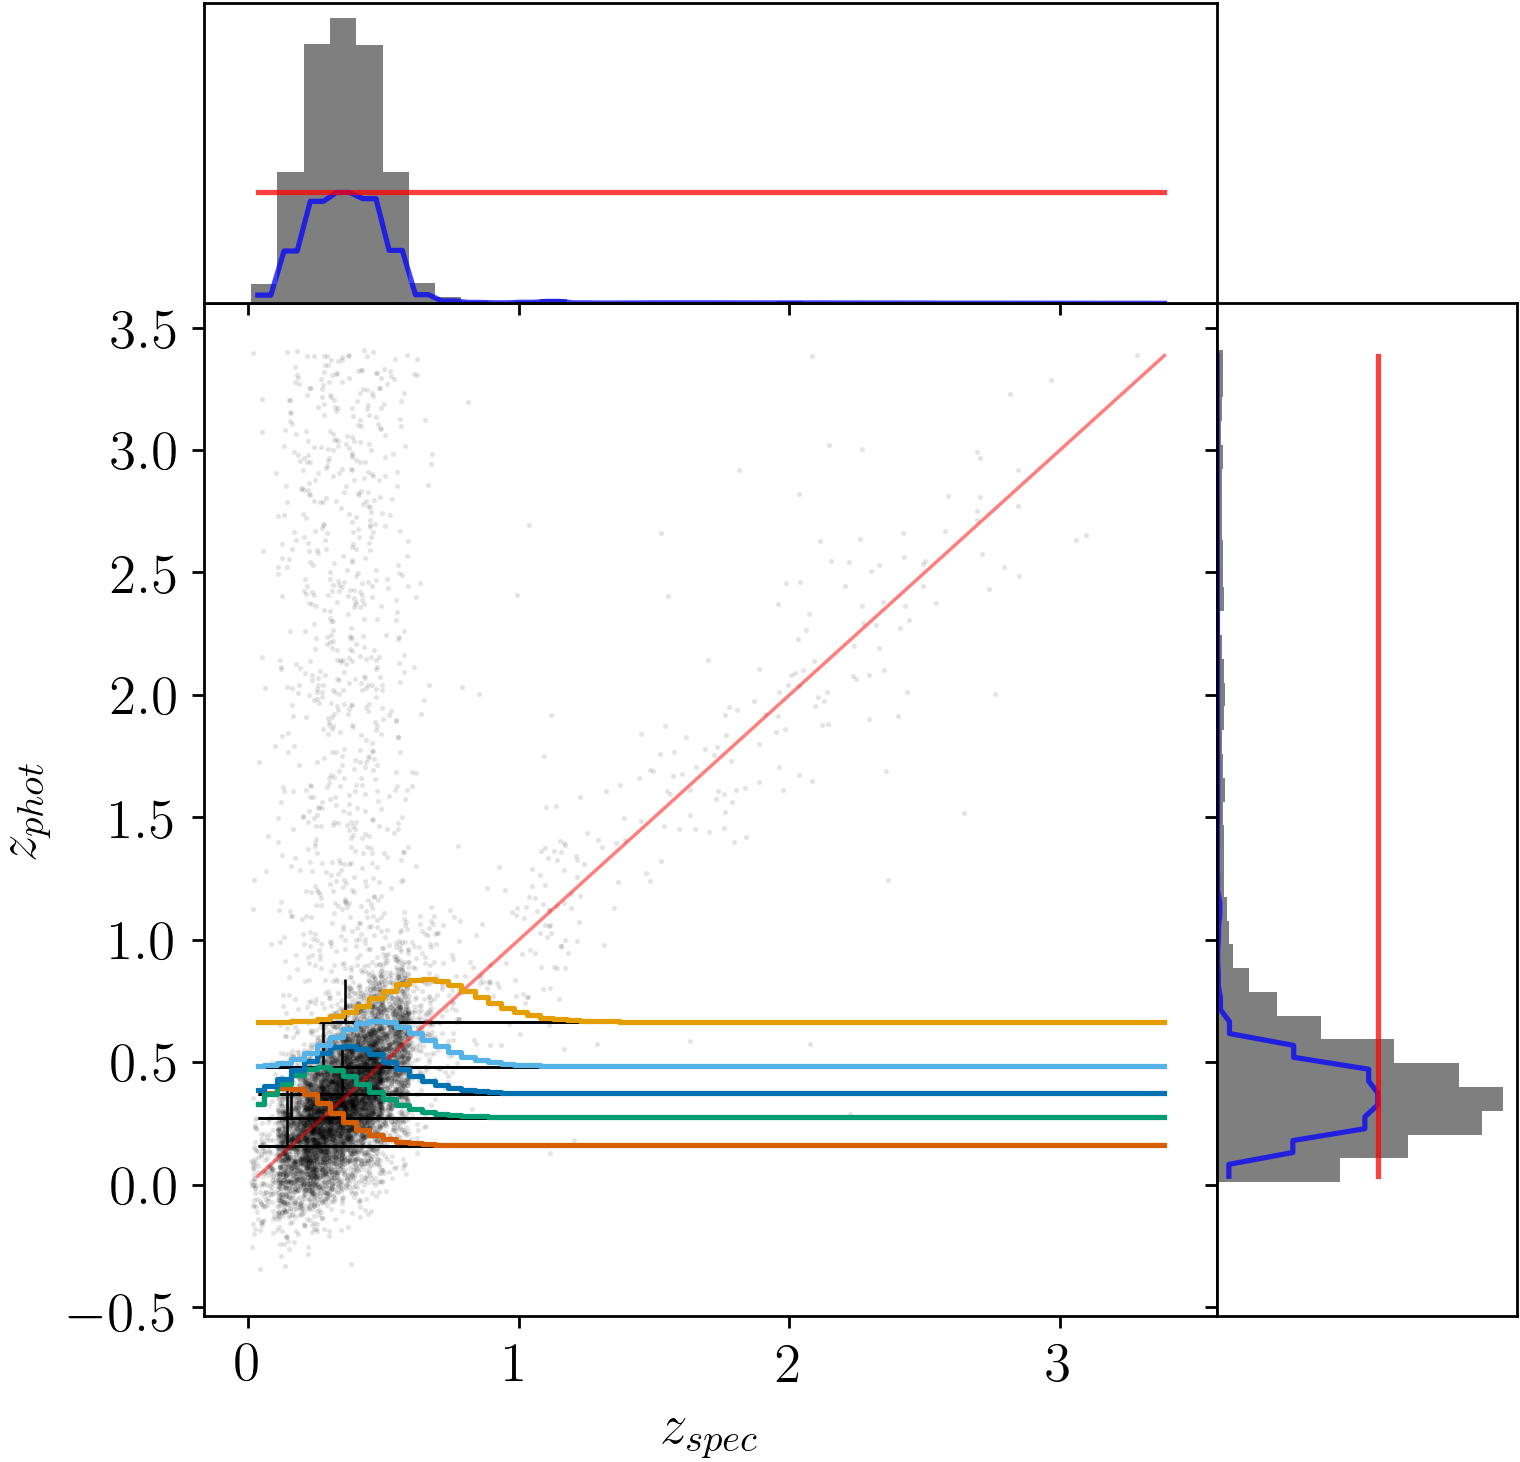
\includegraphics[width=0.24\textwidth]{figures/chippr/0single_lsst_mega_scatter.png}
		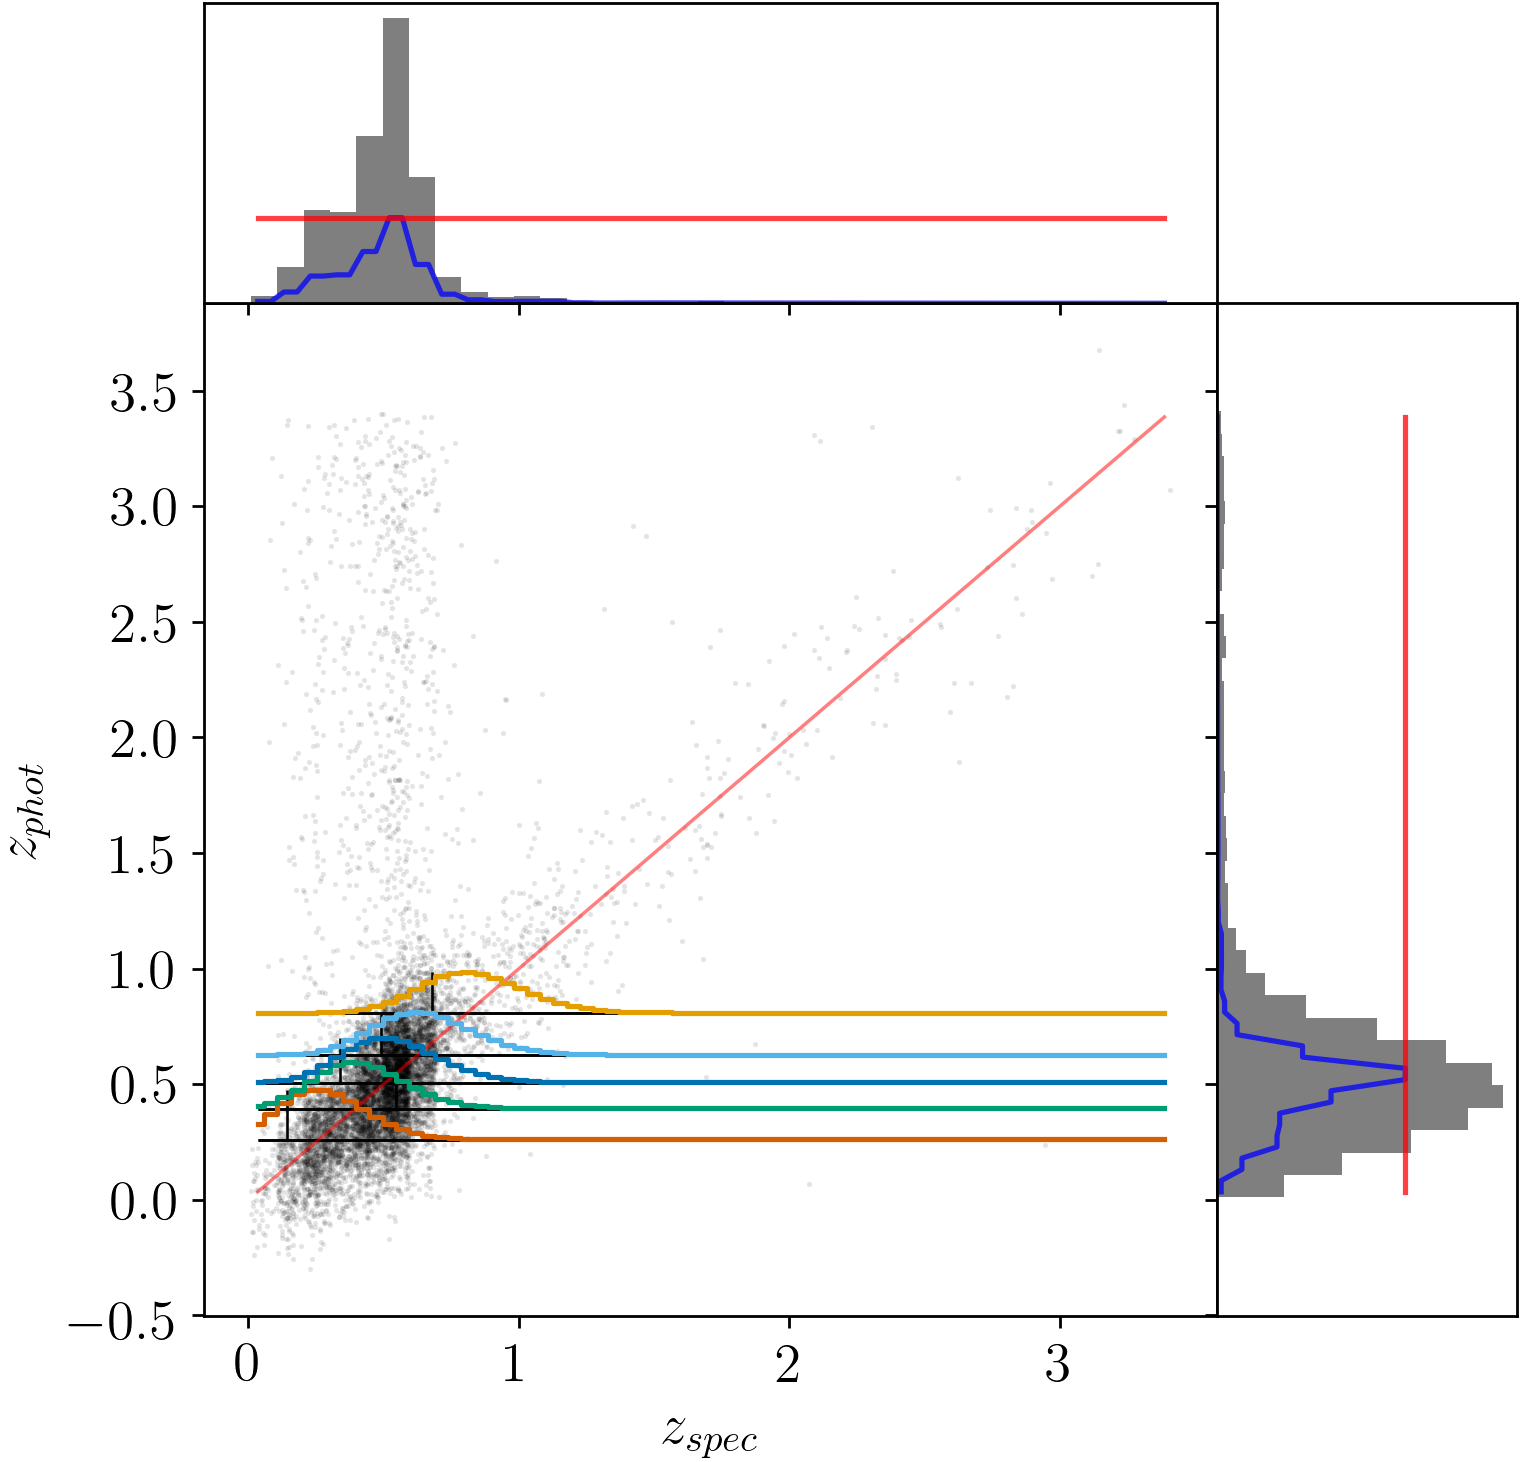
\includegraphics[width=0.24\textwidth]{figures/chippr/1single_lsst_mega_scatter.png}
		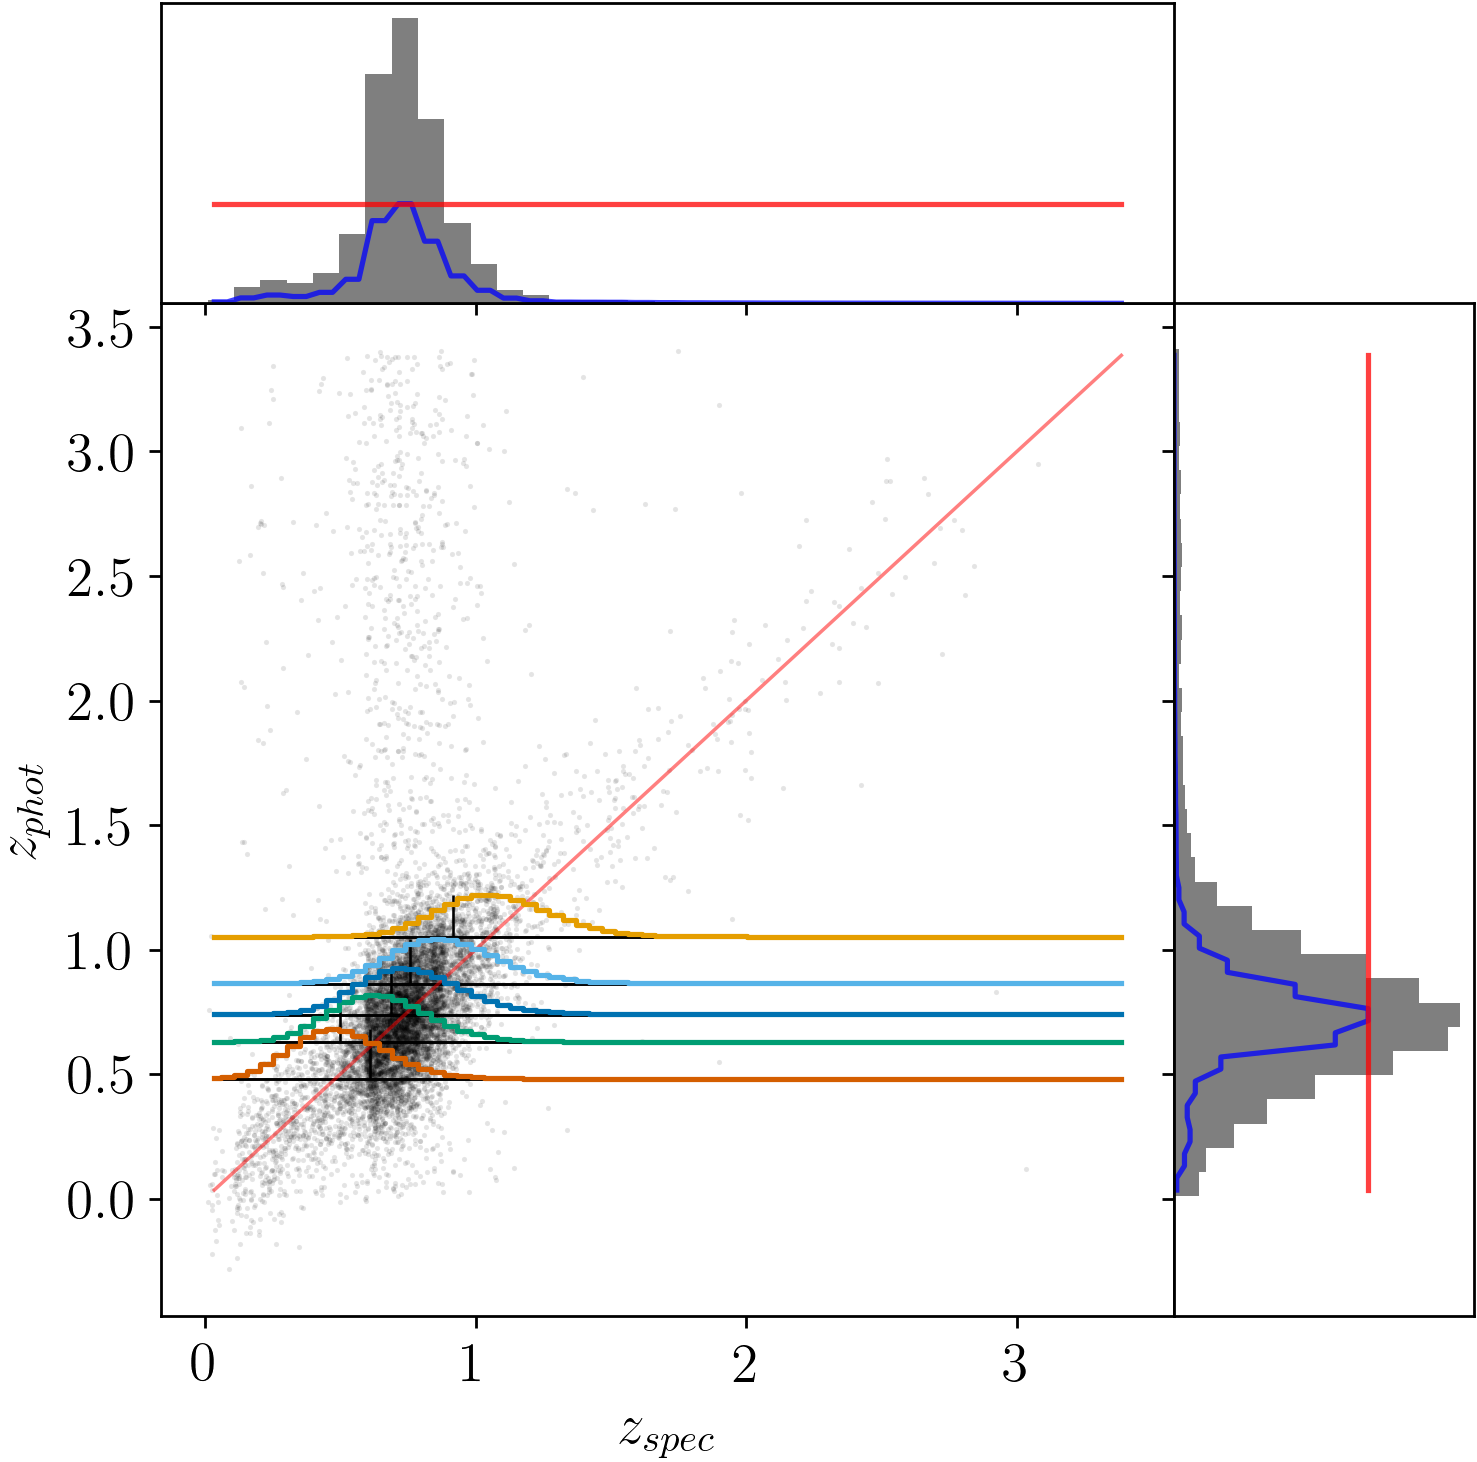
\includegraphics[width=0.24\textwidth]{figures/chippr/2single_lsst_mega_scatter.png}
		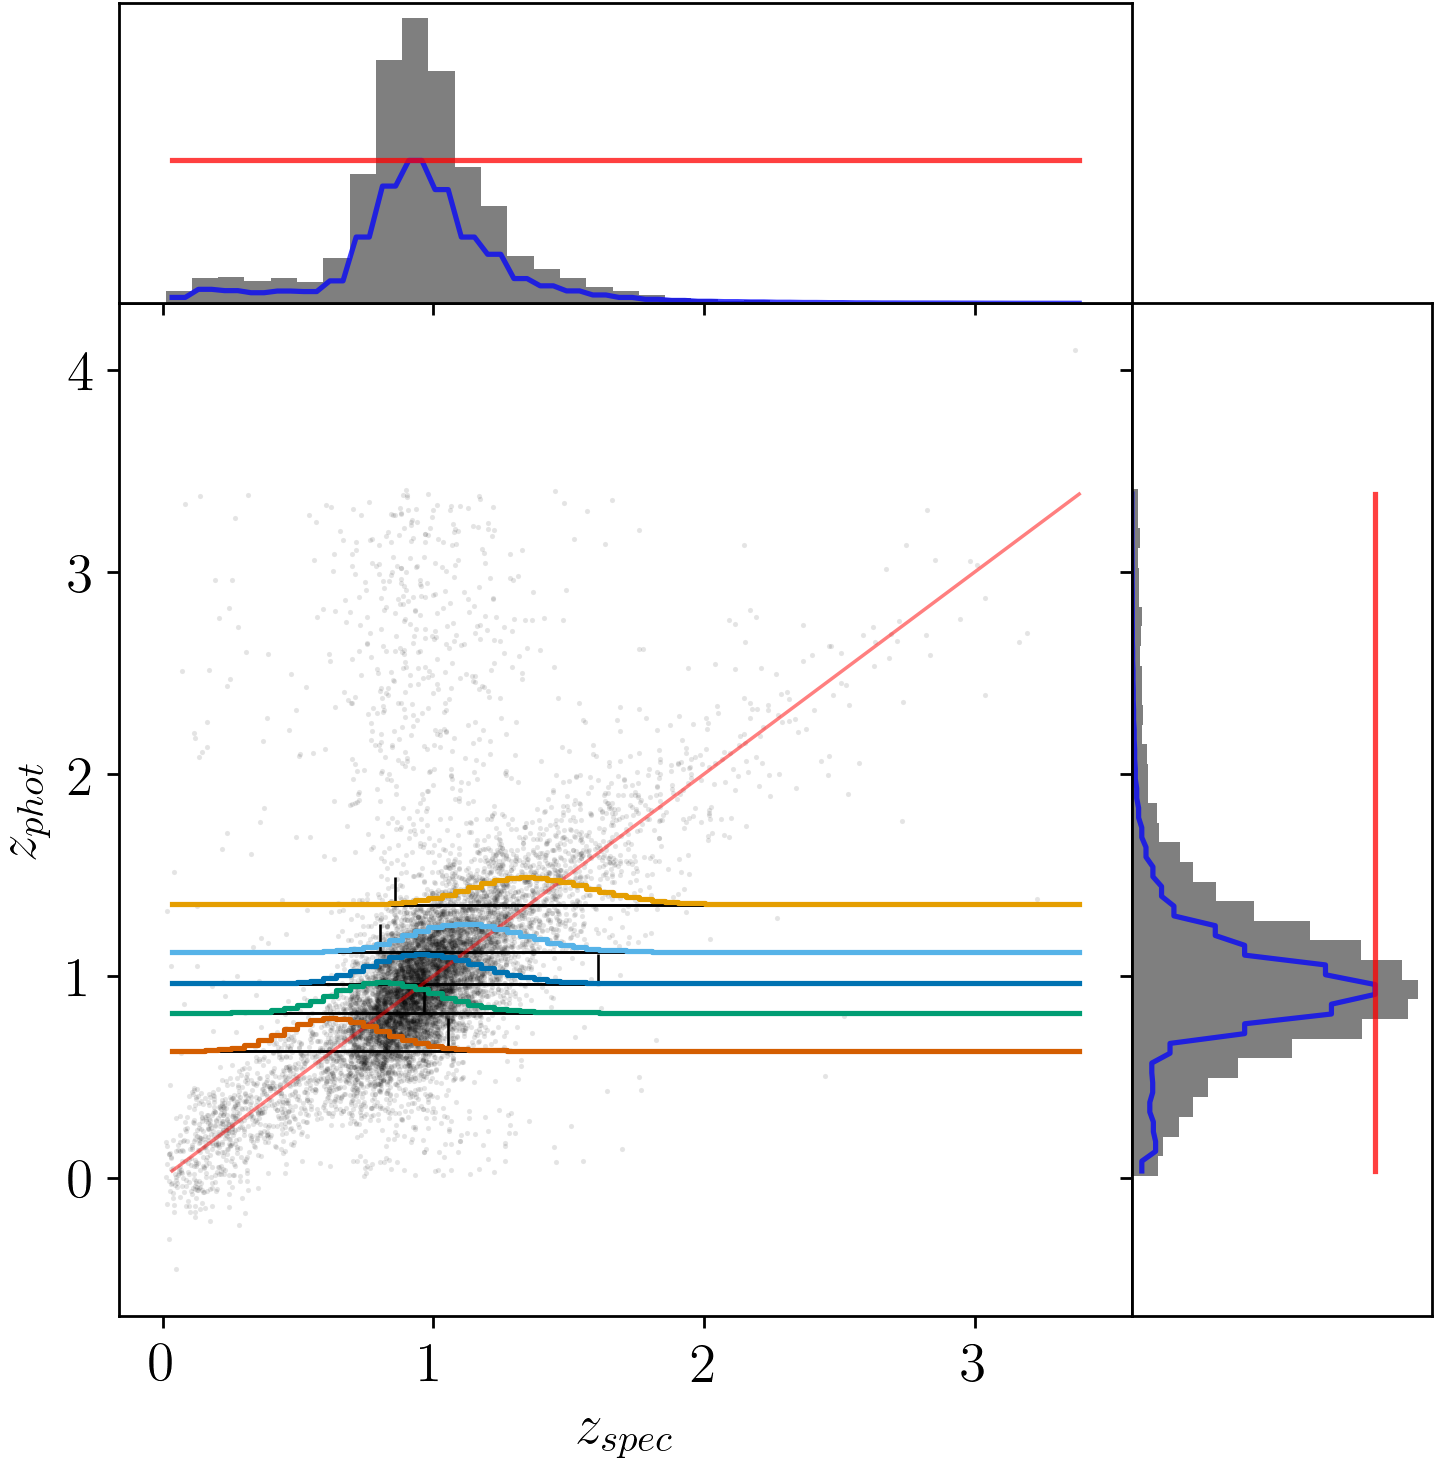
\includegraphics[width=0.24\textwidth]{figures/chippr/3single_lsst_mega_scatter.png}
		\caption{As in \Fig{fig:mega_scatter}, with a different tomographic bin in each panel and the three effects of intrinsic scatter, uniformly distributed catastrophic outliers, and bias at the levels of the \lsst\ SRD, given in Table~\ref{tab:lsstsrd}.
		\aim{TODO: Make this one big plot instead of four little ones to eliminate repeated insets and legend.
		Enlarge axis labels.
		Label panels.
		Also, add watermark of ``mock data'' in UL corner, same for ``results of inference'' on other kind of plot.}
		}
		\label{fig:per-bin-scatter}
	\end{center}
\end{figure*}

\que{Is the distinction between binned samples determined by some observational property and probabilistic redshift distributions sufficiently clear?}

We then make a point estimate of \nz\ using \chippr's \mmle\ optimization option as well as the alternative methods on the \pzpdf\ catalog for each tomographic bin, shown in \Fig{fig:per-bin-ests}, because \cosmolike\ produces cosmology constraints from a single \nz\ result, rather than samples from the full posterior probability density of possible \nz.
Note that \Fig{fig:per-bin-ests} is shown in linear rather than log probability units, unlike all other plots in this paper, to better show the behavior at low probability.
The excessive breadth of the alternative estimators can be seen quite plainly.

\begin{figure*}
	\begin{center}
		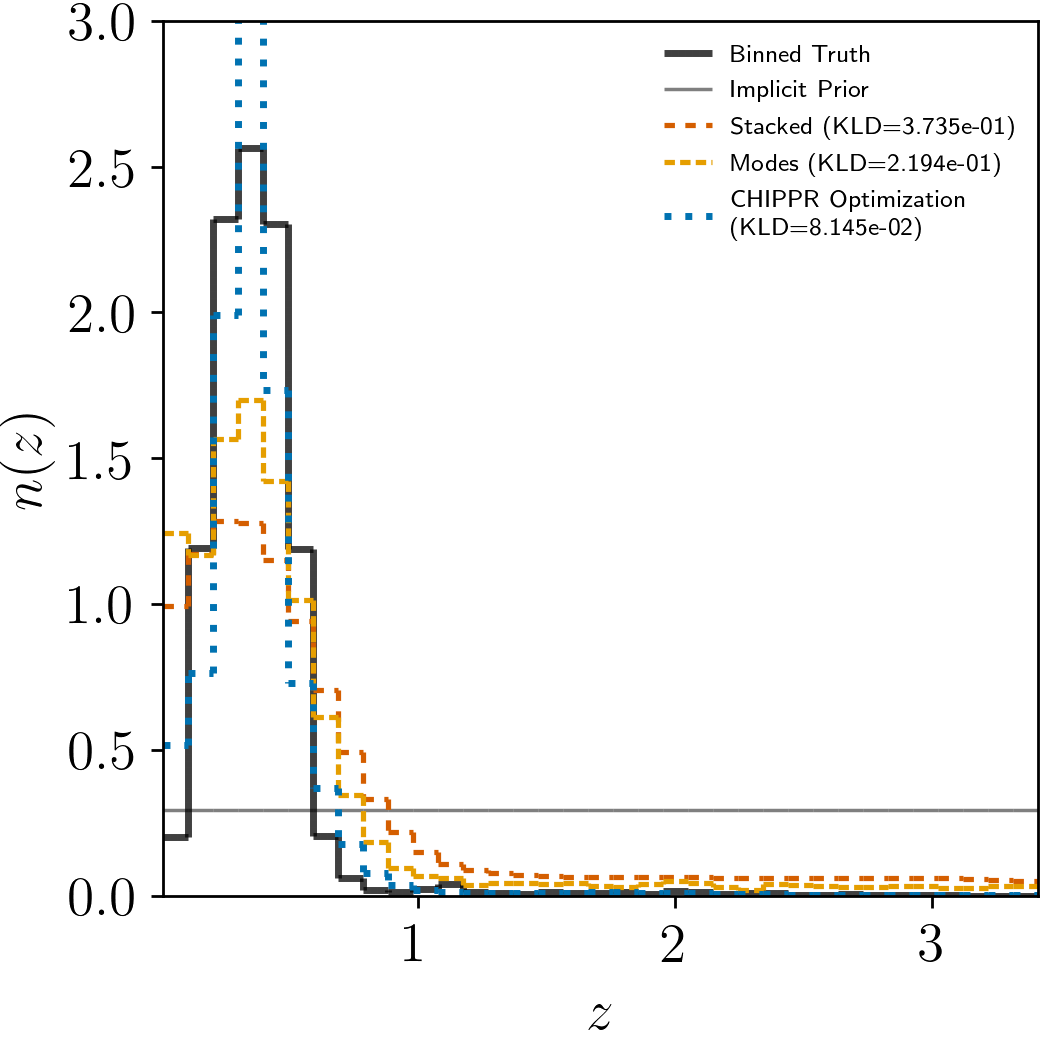
\includegraphics[width=0.24\textwidth]{figures/chippr/0single_lsst_lin_estimators.png}
		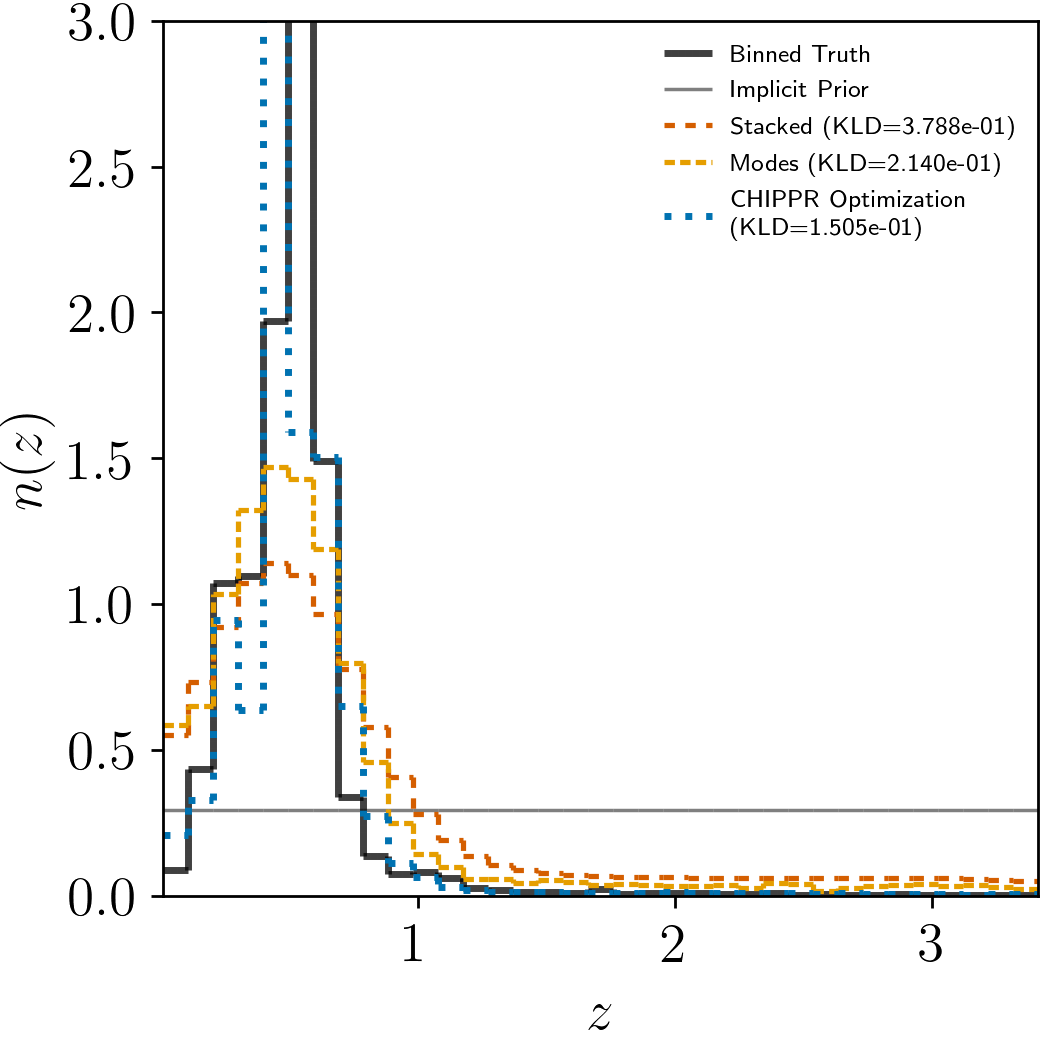
\includegraphics[width=0.24\textwidth]{figures/chippr/1single_lsst_lin_estimators.png}
		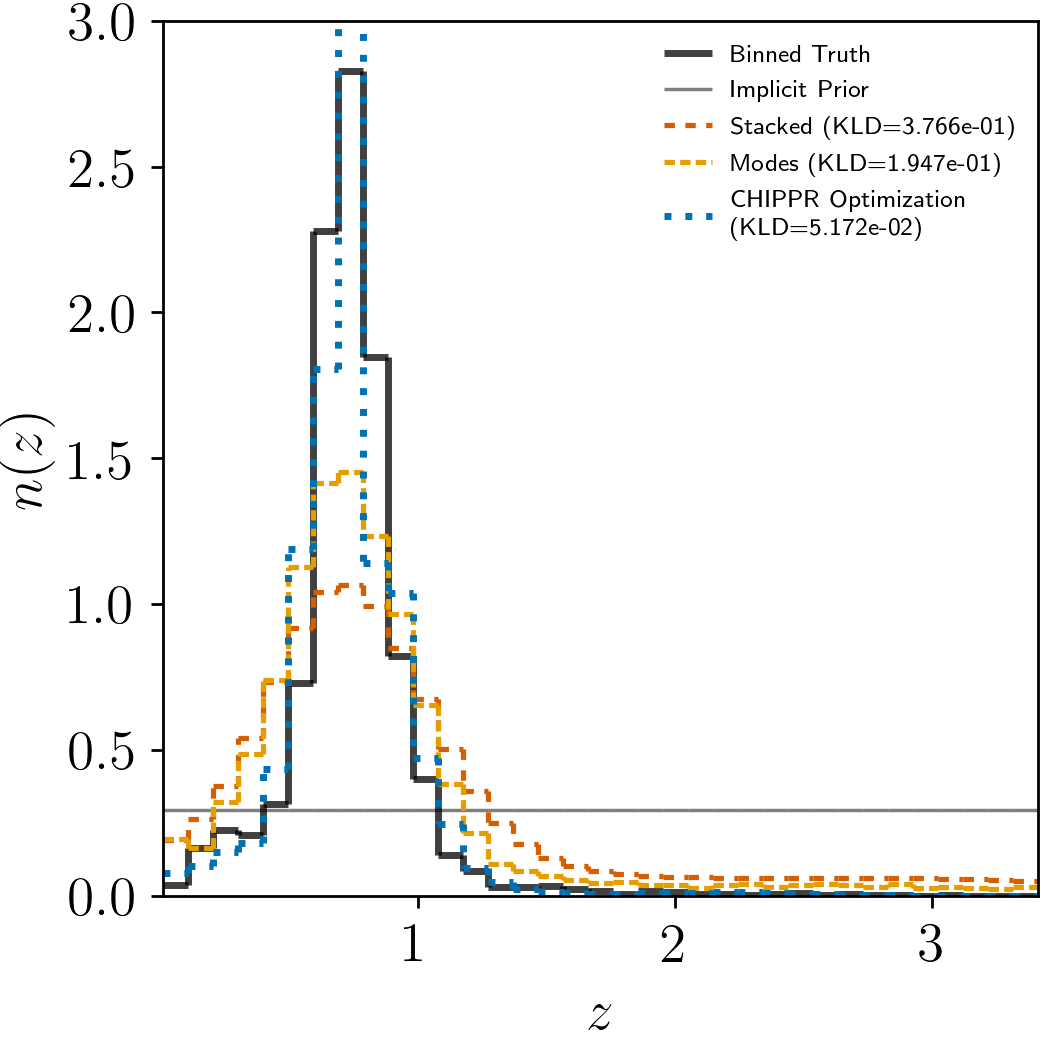
\includegraphics[width=0.24\textwidth]{figures/chippr/2single_lsst_lin_estimators.png}
		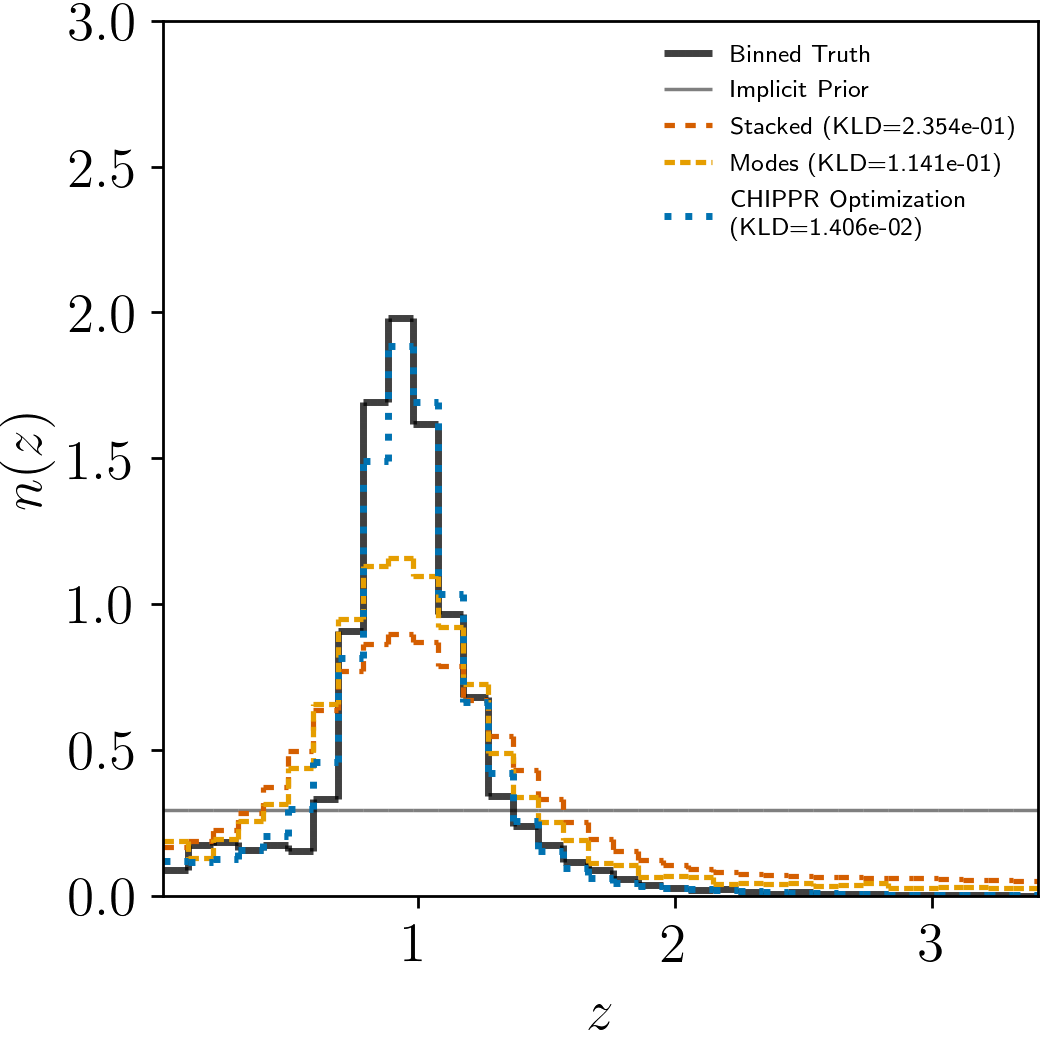
\includegraphics[width=0.24\textwidth]{figures/chippr/3single_lsst_lin_estimators.png}
		\caption{
			The \chippr-derived and other estimators of \nz\ in each tomographic bin, with the true \nz\ (black), the implicit prior (gray), stacked estimator (red), histogram of modes (yellow), and \Chippr\ \mmle\ (blue).
			The result of stacking is far too broad for \lsst-like \pzpdf s, even moreso than the simplistic histogram of modes.
			\aim{TODO: Make this one big plot instead of four little ones to eliminate repeated axis labels and legend.
			Label figure/panels.
			Also, add watermark of ``results of inference'' in UL corner, same for ``mock data'' on other kind of plot.}
		}
		\label{fig:per-bin-ests}
	\end{center}
\end{figure*}

We then use the different estimators of \nz\ in a cosmological forecasting procedure with \cosmolike, constraining $\Omega_{m}$, $\Omega_{b}$, $w_{a}$, $w_{0}$, $n_{s}$, $S_{8}$, and $H_{0}$.
Though there are also slight differences in the angle of the error ellipses, the most striking effect is the broadening of the contours under the alternative estimators relative to \Chippr, which are almost indistinguishable from those derived by using the true redshift distribution in each bin.
The stacked estimator is significantly worse than the \Chippr\ \mmle\ for all parameters except $\Omega_{b}$ and $H_{0}$.
Stacking, however, outperforms the histogram of modes for all parameters except $\Omega_{m}$ and $S_{8}$, for which their constraints are quite similar.
Though the true values of the parameters themselves were not accessible with the Fisher matrix-based framework, we calculate the seven-dimensional KLD for the three \nz\ estimators relative to the constraints derived from the true \nz, showing that \Chippr\ preserves information $200-800$ times better than the alternatives, with the histogram of modes doing about four times better than stacking.
%\aim{TODO: Ask Elisabeth how to get the bias here.}
\que{So a Fisher matrix analysis inherently can't provide the bias, because that requires data.
Because we have no data, only posteriors conditioned on hypothetical data, this isn't possible.
Do you think it's sufficient to provide the bias on the moments of \nz, since that's what everyone uses anyway?}

\begin{figure*}
	\begin{center}
		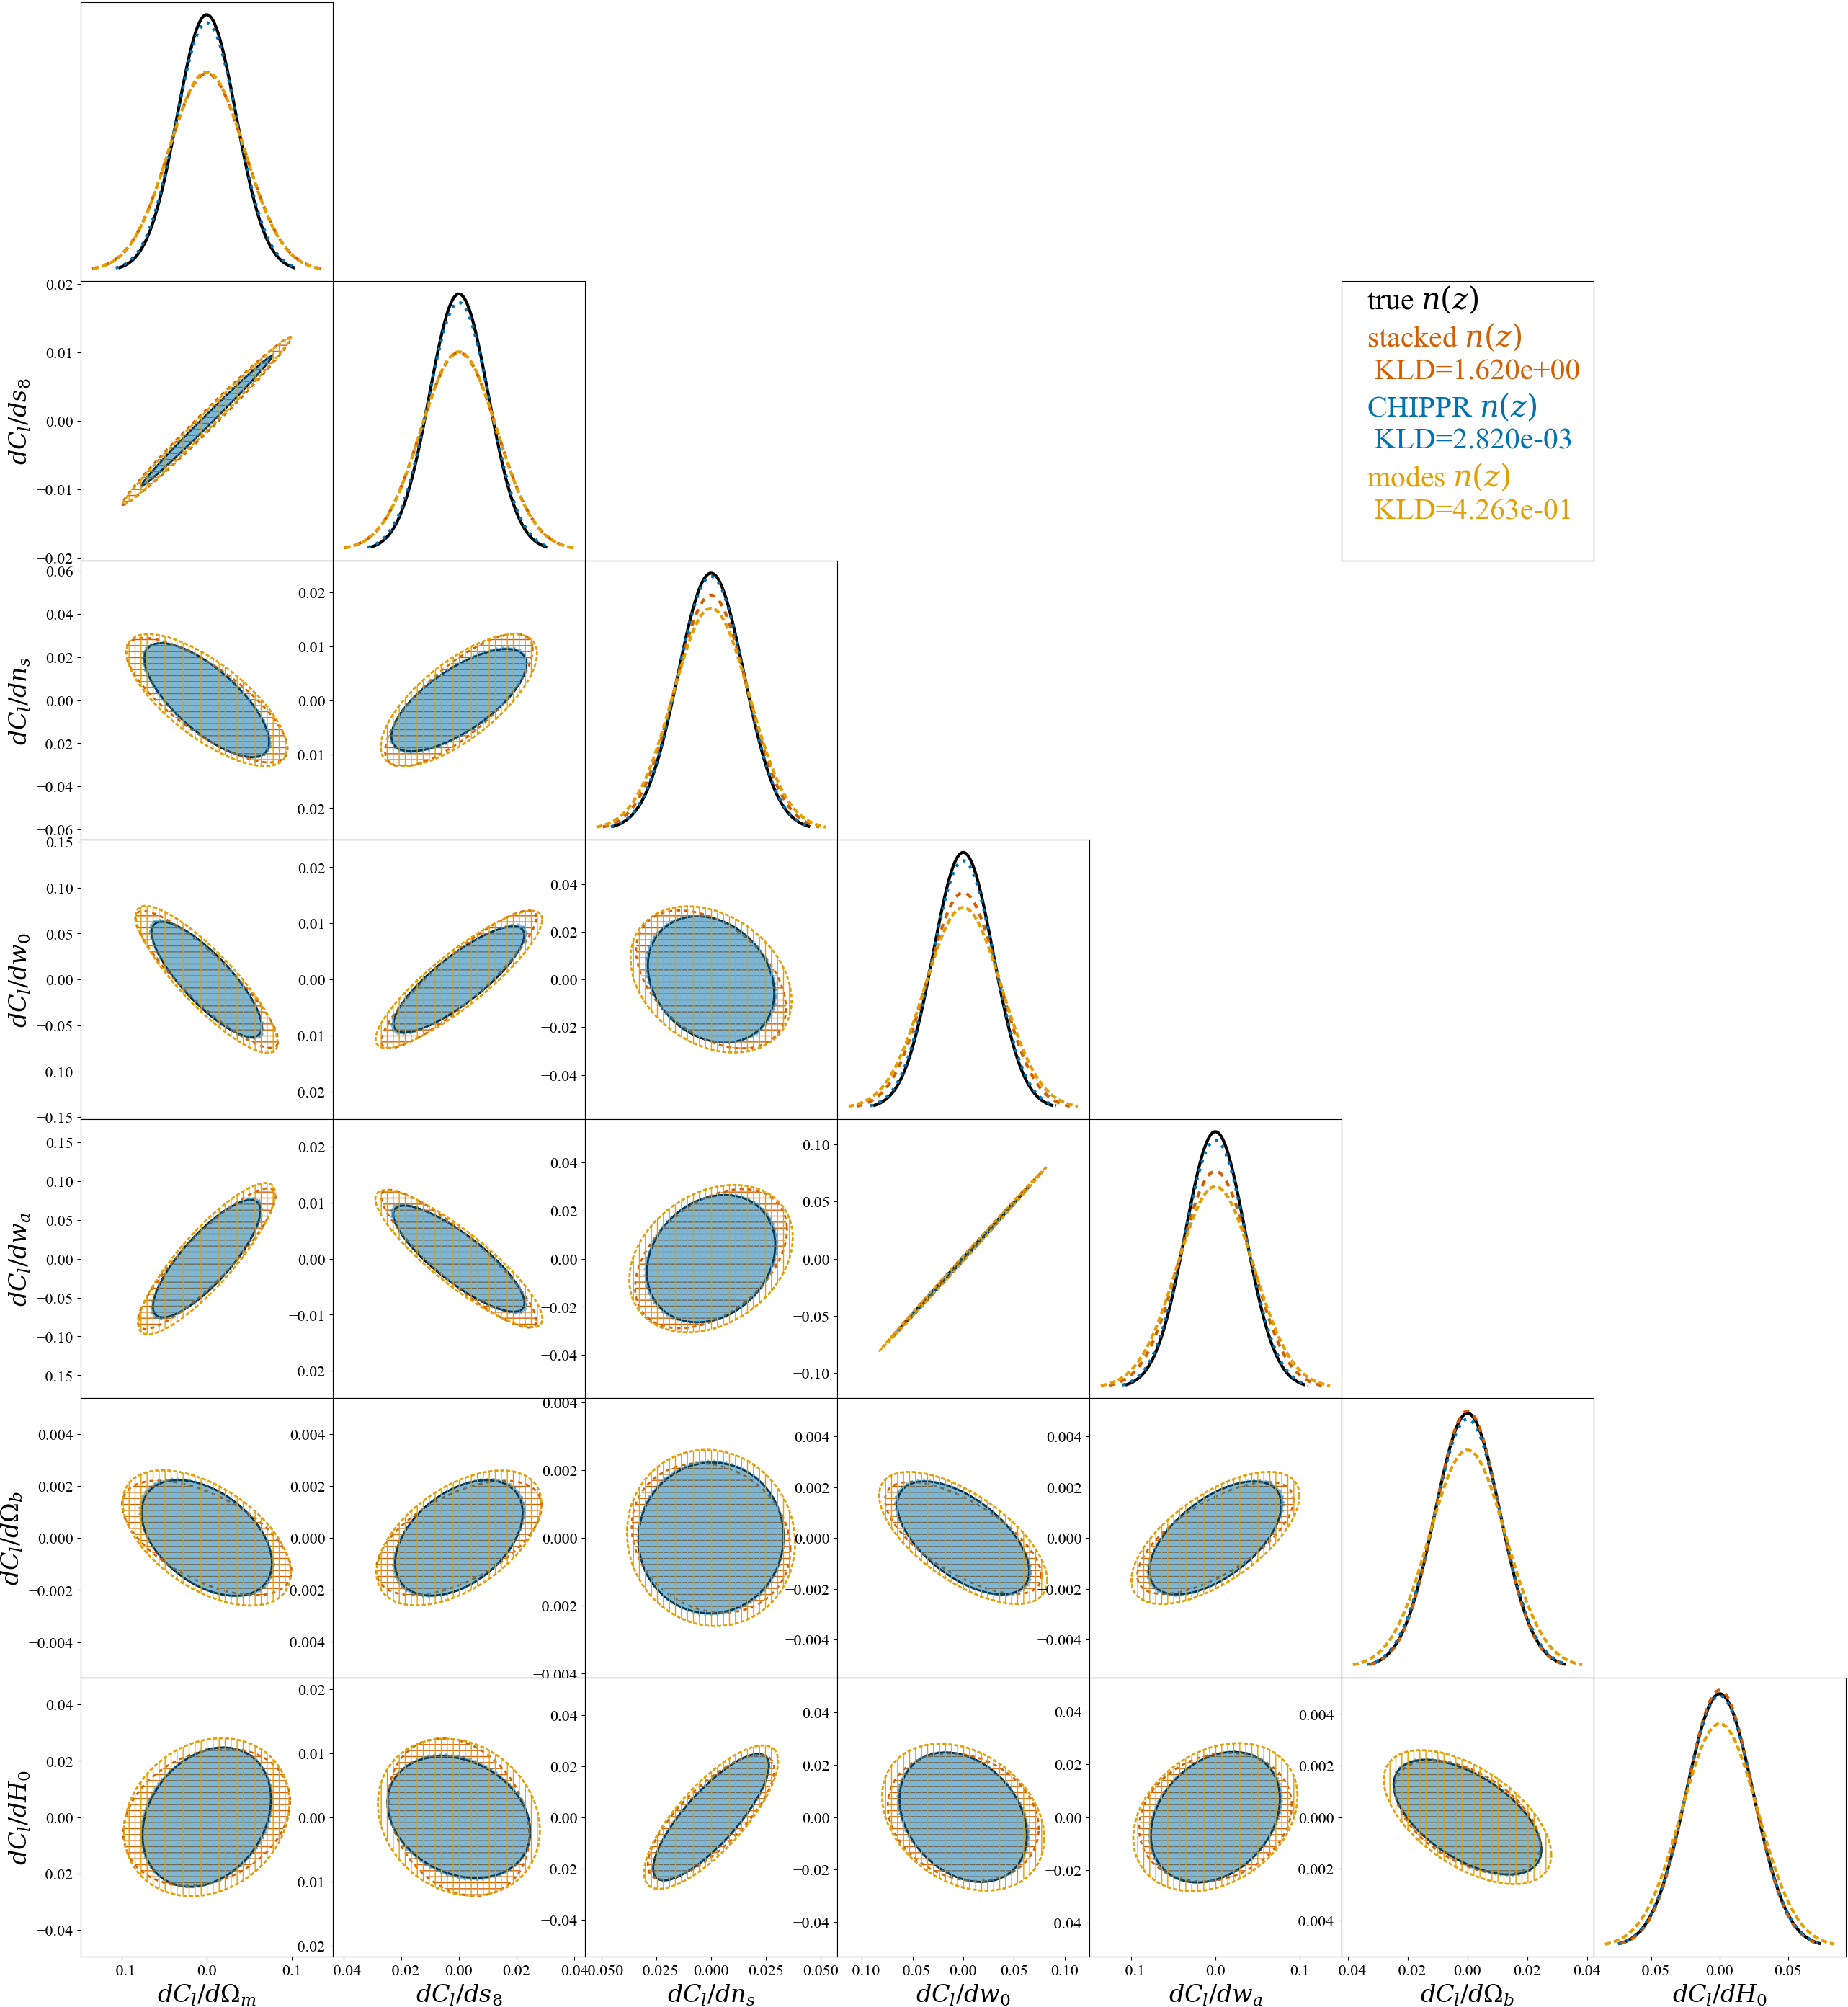
\includegraphics[width=0.9\textwidth]{figures/chippr/final_plot.png}
		\caption{
			\que{Are the contours any easier to see now?}
			The result of propagating the estimators of \nz\ by stacking (red), the histogram of modes (yellow), \Chippr\ (blue), and the true \nz\ (black) of \Fig{fig:per-bin-ests} to a subset of cosmological parameters.
			For all parameters considered, \Chippr\ yields contours no broader than those corresponding to the true \nz, whereas for most parameters, stacking and the histogram of modes yield broader contours.
			\aim{TODO: Fix formatting of axis labels.
			Standardize ticklabels.}
		}
		\label{fig:cornerplot}
	\end{center}
\end{figure*}

\que{Does this discussion adequately quantify how good \Nz\ has to be and how wrong we'll be if we estimate it wrong?
	Suggestions for how to better establish context would be appreciated.}

\subsection{Violations of the model}
\label{sec:violations}

\que{Move \Sect{sec:interim} here?}

In this test, without tomographic binning, the \pzip s are made to the \lsst\ requirements but the implicit prior used for the inference is not the same as the implicit prior used for generating the data.
\Pzpdf\ codes do not generally provide their implicit prior, with the exception of some template-fitting techniques for which it is a known input.
If we naively used the \pzpdf\ catalog produced by a generic machine learning code and assumed a flat implicit prior, we would observe the contents of \Fig{fig:mischaracterized}.

\begin{figure}
	\begin{center}
		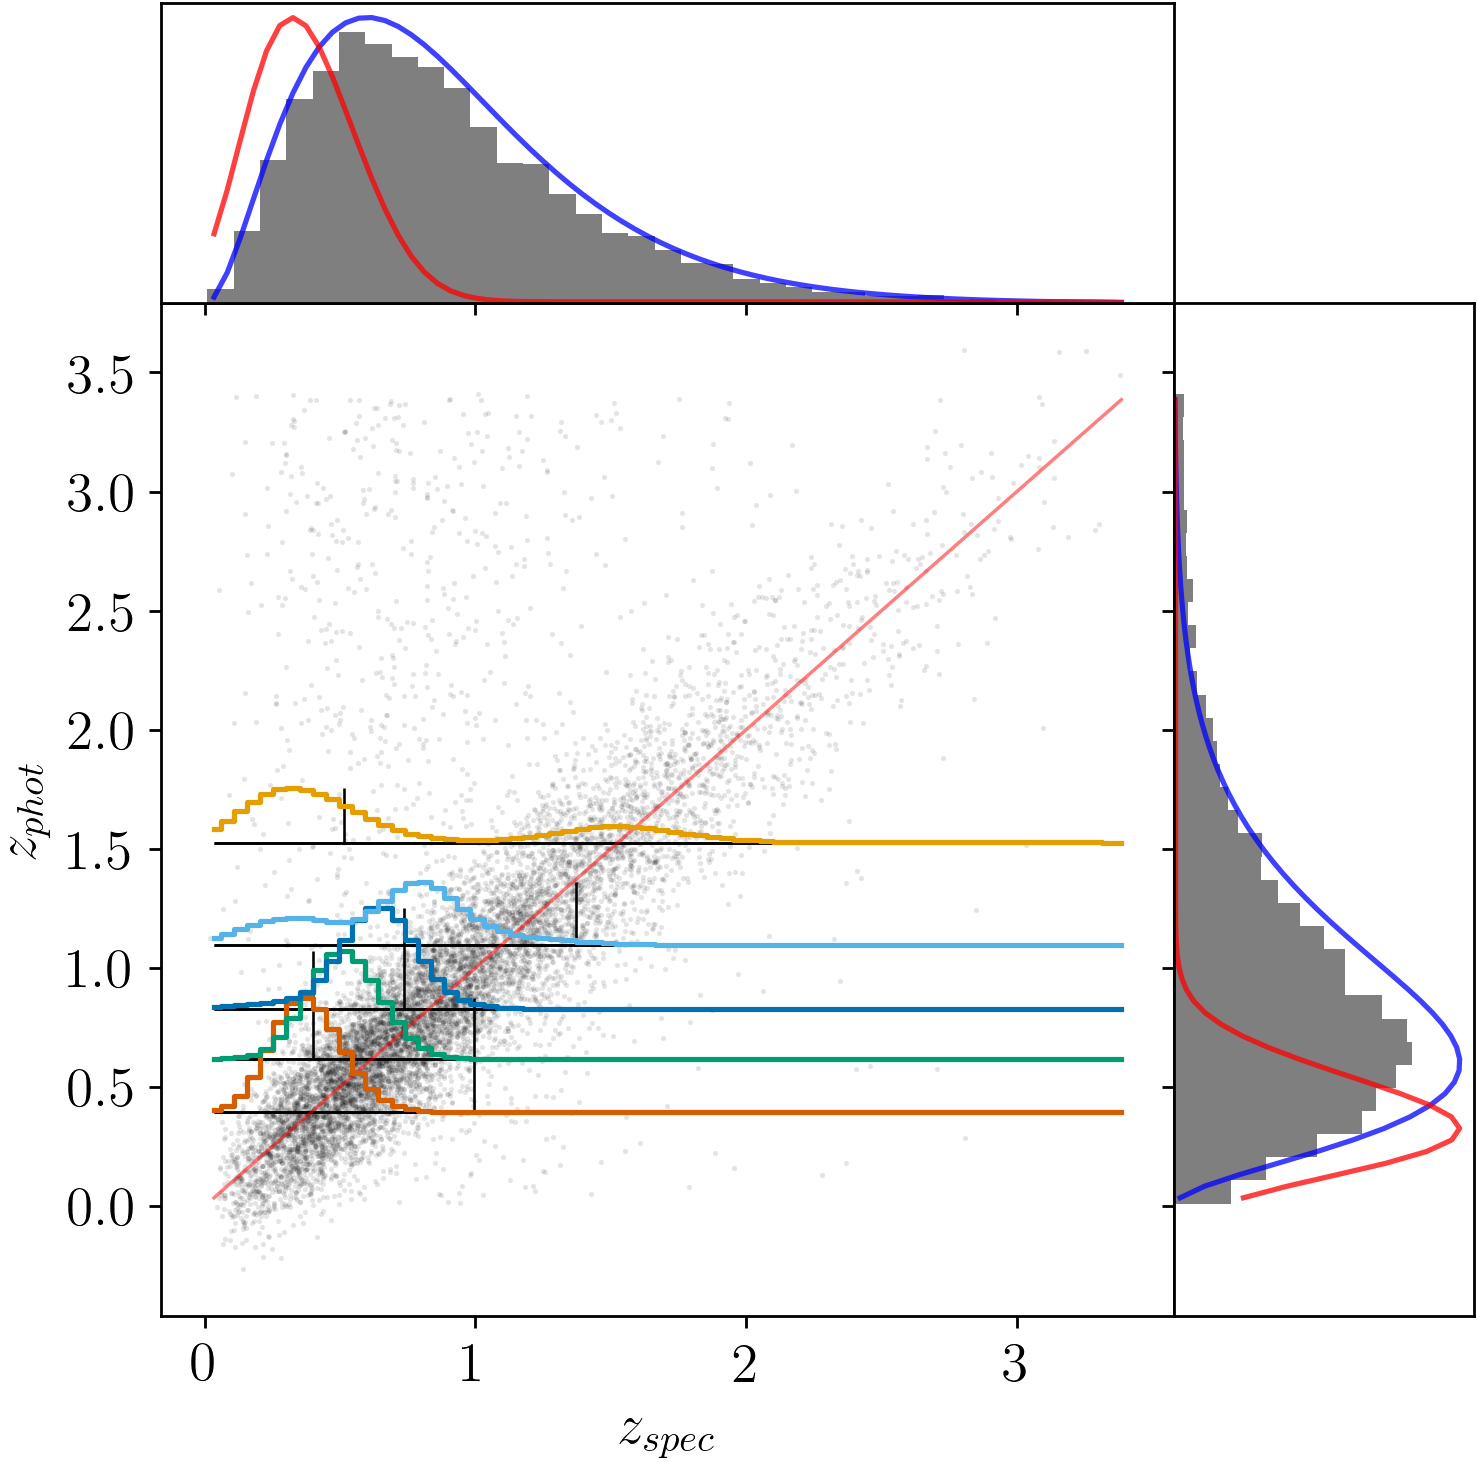
\includegraphics[width=0.45\textwidth]{figures/chippr/misspecified_mega_scatter.png}\\
		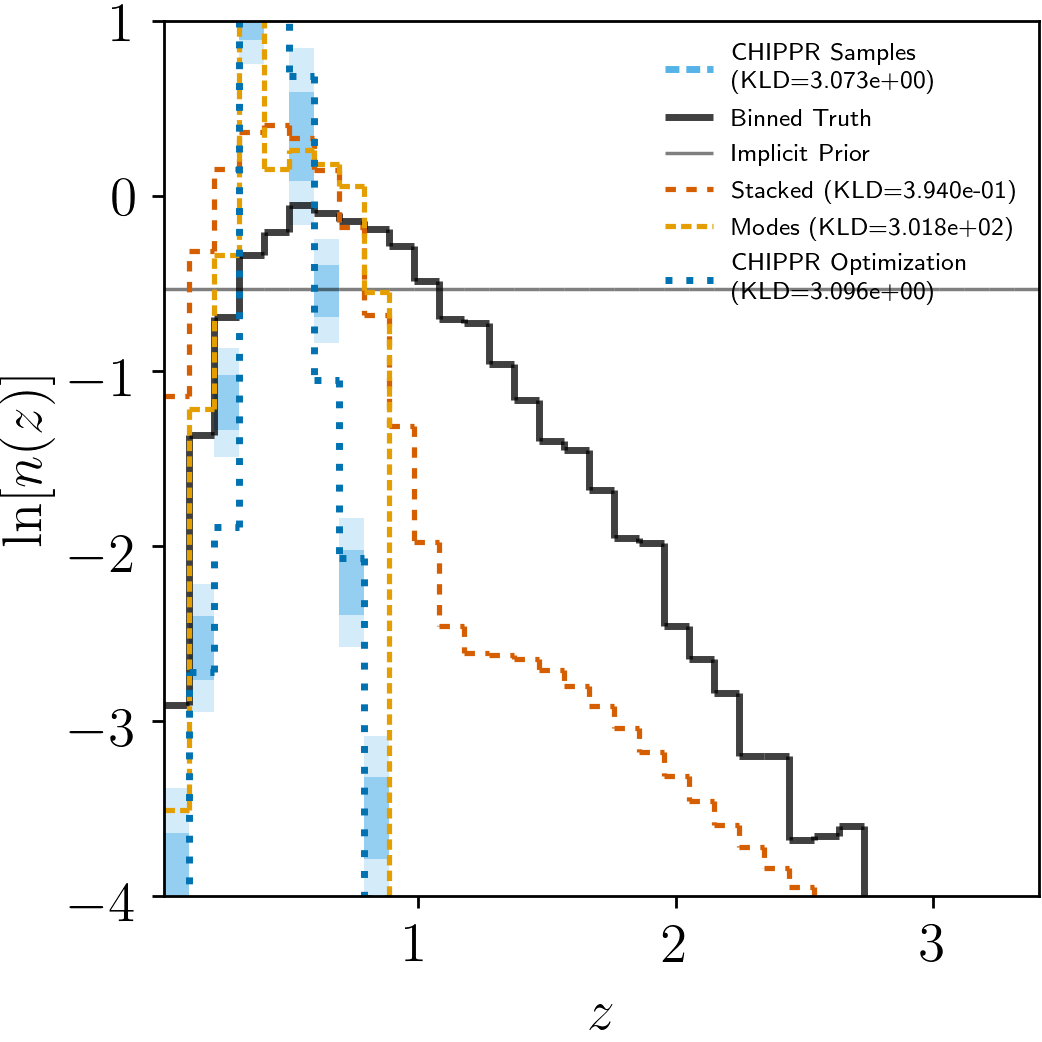
\includegraphics[width=0.45\textwidth]{figures/chippr/misspecified_log_estimators.png}
		\caption{
			Top: Examples of \pzpdf s with systematics at the level of the \lsst\ requirements with a machine learning-like implicit prior, including samples from the probability space of true and observed redshift (black points), \pzpdf s (colored curves), and the true redshifts of the example \pzpdf s (black vertical lines), with marginal histograms (gray) for each dimension with the true redshift distribution (blue curve) and implicit prior (red curve) in the insets.
			Bottom: The results of \Chippr\ (samples in light blue, optimization in dark blue) and the alternative approaches (the stacked estimator in red, the histogram of modes in yellow) on \pzpdf s with uniformly distributed catastrophic outliers, with the true redshift density (black curve) and the uniform implicit prior given to \chippr\ (gray curve).
			When the incorrect implicit prior is provided to \chippr, even Bayesian inference cannot recover the true \nz.
			\aim{TODO: Enlarge axis labels on top.
			Label panels/figure.
			Also, add watermark of ``mock data'' in UL corner of top panel and ``results of inference'' on bottom panel.}
		}
		\label{fig:mischaracterized}
	\end{center}
\end{figure}

The results of using a mischaracterized implicit prior are disastrous, causing every estimator, including \Chippr, to be strongly biased.
The stacked estimator and histogram of modes don't make use of the implicit prior so do no worse than when the implicit prior is accurately provided, but \Chippr\ is sensitive to prior misspecification, which violates the model upon which it is based.
It is thus crucial that \pzpdf\ methods always characterize and provide the implicit prior.

% removed ancient investigation on real data, would be hard to redo with the new \chippr\ code on this timescale given that I haven't even looked at the data format in 4 years

\section{Conclusion}
\label{sec:con}

This study derives and demonstrates a mathematically consistent inference of a one-point statistic, the redshift density function \nz, based on an arbitrary catalog of \pzpdf s.  
The fully Bayesian method, based in the fundamental laws of probability, begins with a probabilistic graphical model corresponding to equations for the full posterior distribution over the parameters for \nz.  
The method is validated on mock data and tested in the regime of \lsst\ with promising results, outperforming the traditional stacking estimator at the level of \nz\ as well as in terms of constraining power on the cosmological parameters.
Not only is this the only mathematically correct approach to the problem, it also recovers the true parameter values better than popular alternatives, as measured by the loss of information in \nz\ and the size of error ellipses in the space of cosmological parameters.

%In the tests on simulated data performed here, the full posterior distribution over the hyperparameters defining $N(z)$ derived by this method is consistent with the true redshift distribution function, making the mean of sampled values an excellent point estimator of $N(z)$.  
%The information contained in the full posterior distribution's shape convey the traditional error bar information without having to explicitly propagate any error estimates.  
\aim{TODO: Refer to quantitative results on KLD of \Nz\ and cosmological parameter space.}
%The results of those tests is summarized below and in \Tab{tab:kld}, where lower values indicate a closer match between the true $N(z)$ and the estimator.  
%Tests were also performed on subsets of BOSS DR10 data with results consistent with those of simulations.

\dwh{\Chippr\ outperforms traditional estimators of \nz\ under the canonical \pz\ systematics of intrinsic scatter, catastrophic outliers, and bias.
\Chippr\ is also robust to nontrivial implicit priors corresponding to the specifics of the architecture of the method by which \pzpdf s are obtained.
However, \Chippr\ absolutely requires that the implicit prior is accurately known; using an implicit prior other than that which contributed to the production of the \pzpdf\ catalog results in catastrophically incorrect inference of \nz.
It is therefore imperative that those developing codes to obtain \pzpdf s provide a way to isolate the implicit prior and that those publishing \pzpdf\ catalogs provide the implicit prior to users.

This mandate is easier said than done, both for template fitting and machine learning approaches.
While the implicit prior is often an explicit input to model-based routines, it may be defined in a space of redshift and SED templates.
In this case, it may not be possible to apply \Chippr\ without marginalizing over additional variables $\psi$ for the SEDs.
In other words, obtaining the implicit prior from a template fitting code may be challenging or even require consideration of higher-dimensional PDFs such as $\pr{z, \mathrm{SED} \gvn \psi^{*}}$.

The situation appears more dire for data-driven techniques, whose training sets may not straightforwardly translate into an implicit prior.
For example, some training set galaxies may contribute to the \pzpdf s more than others, resulting in different effective weights when factoring into, say, a histogram of training set redshifts as the implicit prior.
Additionally, the weights may be stochastic, depending on the random seed used to initialize non-deterministic methods, precluding reproducibility.
It is thus unclear whether the implicit prior can be meaningfully obtained from such methods at all.

\aim{TODO: new paragraph for what can go wrong, call to community for what to do about it, what aspects of implicit prior are knowable and not knowable?
	if testable how so? outside the scope of paper, data producers be warned!
	a likelihood is better -- give us that if you can!
	focus on methods that acknowledge probabilistic structure of problem}

A thorough investigation of the degree to which the implicit prior can be meaningfully obtained is outside this paper but should be a priority for all consumers of \pzpdf s.
As an alternative, however, we must point out that if likelihoods were available rather than posteriors, the trouble with the implicit prior would be avoided altogether.
We thus encourage the community of those making \pzpdf s to consider developing such methods so that the resulting data products may be correctly used in scientific inference more generically.}

\aim{TODO: claim that implications for tomographic binning are severe, if that can be motivated by Section~\ref{sec:lsstdemo}.}

The following conclusions and recommendations can be made with confidence:

\begin{enumerate}
	\item Both the \Chippr\ \mmle\ and the mean of \chippr\ samples are good point estimators of \nz, whereas the histogram of modes is very sensitive to outliers and the stacked estimator is always excessively broad.
	\item The error bars on the posterior distribution over \nz\ hyperparameters are interpretable and arise naturally under \Chippr, unlike those that may be assumed for the conventional point estimators.
	%	\item The marginalized maximum likelihood estimator is an excellent estimator for strongly featured redshift distribution function with simple, clean photo-$z$ posteriors; stacking smooths features more than sampling and photo-$z$ point estimation.
	\item When the implicit prior is known to be a poor match to the data, only the results of \Chippr\ are satisfactory estimators of the redshift distribution function because they are the only methods that can account for the bias induced on the \pzpdf\ catalog by the method that produces it; this is the most compelling case for the sampler because of the ubiquity of inappropriate interim priors.
\end{enumerate}

By showing that \Chippr\ is effective in recovering the true redshift distribution function and posterior distributions on its parameters from catalogs of \pzpdf s, this work supports the production of \pzpdf s by upcoming photometric surveys such as \lsst\ to enable more accurate inference of the cosmological parameters.  
We discourage researchers from co-adding \pzpdf s or converting them into point estimates of redshift and instead recommend the use of Bayesian probability to guide the usage of \pzpdf s.  
We emphasize to those who produce \pzpdf s from data that it is essential to release the implicit prior used in generating this data product in order for proper inference to be conducted by consumers of this information.
\aim{TODO: Strengthen language and get specific about what \pzpdf\ producers must do.}

The technique herein developed is applicable with minimal modification to other one-point statistics of redshift to which we will apply this method in the future, such as the redshift-dependent luminosity function and weak lensing mean distance ratio.  
Future work will also include the extension of this fully probabilistic approach to higher-order statistics of redshift such as the two-point correlation function.

\appendix
%\renewcommand{\thesection}{\Alph{section}}
%\renewcommand{\thesubsection}{\Alph{subsection}}

\aim{TODO: Figure out how to get the appendices enumerated for reference earlier.}

\section{Derivation}
\label{app:math}

\aim{TODO: make notation consistent with the rest of the paper.}

%We begin by parametrizing $N(z)$ in terms of $\vec{\theta}$, comprising some set of hyperparameters that define the form $N(z)$ may take in whatever basis we choose.  
%We define a function $f_{\vec{\theta}}(z)=N(z)$ that transforms these hyperparameters into the redshift distribution function $N(z)$.  
%Because 
%\begin{equation}
%\eqlabel{eq:definition}
%N(z) \propto p(z \gvn \vec{\theta}),
%\end{equation}
%we may discontinue discussion of $N(z)$ in favor of the likelihood $p(z|\vec{\theta})$.

In this paper, we work exclusively with log-probabilities.  
What we wish to estimate is then the full log-posterior probability distribution (hereafter the full log-posterior) of the hyperparameters $\ndphi$ given the catalog of photometry $\{\data_{j}\}$.

By Bayes' Rule, the full log-posterior
\begin{equation}
\label{eqn:basicbayes}
\ln[\pr{\ndphi \gvn \{\data_{j}\}}] = \ln[\pr{\{\data_{j}\} \gvn \ndphi}] + \ln[\pr{\ndphi}] - \ln[\pr{\{\data_{j}\}}]
\end{equation}
may be expressed in terms of the full log-likelihood probability distribution (hereafter the full log-likelihood) $\ln[\pr{\{\data_{j}\} \gvn \ndphi}]$ by way of a hyperprior log-probability distribution (hereafter the hyperprior) $\ln[\pr{\ndphi}]$ over the hyperparameters and the log-evidence probability of the data $\ln[\pr{\{\data_{j}\}}]$.
However, the evidence is rarely known, so we probe the full log-posterior modulo an unknown constant of proportionality.

The full log-likelihood may be expanded in terms of a marginalization over the redshifts as parameters, as in 
\begin{equation}
\label{eqn:marginalize}
\ln[\pr{\{\data_{j}\} \gvn \ndphi}] = \ln\left[\integral{\pr{\{\data_{j}\} \gvn \{z_{j}\}} \pr{\{z_{j}\} \gvn \ndphi}}{\{z_{j}\}}\right].
\end{equation}

We shall make two assumptions of independence in order to make the problem tractable; their limitations are be discussed below.  
First, we take $\ln[\pr{\{\data_{j}\} \gvn \{z_{j}\}}]$ to be the sum of $J$ individual log-likelihood distribution functions $\ln[\pr{\data_{j} \gvn z_{j}}]$, as in 
\begin{equation}
\label{eqn:indiedat}
\ln[\pr{\{\data_{j}\} \gvn \{z_{j}\}}] = \sum_{j=1}^{J}\ \ln[\pr{\data_{j} \gvn z_{j}}],
\end{equation}
a result of the definition of probabilistic independence encoded by the box in \Fig{fig:pgm}.
Second, we shall assume the true redshifts $\{z_{j}\}$ are $J$ independent draws from the true $\pr{z \gvn \ndphi}$.  
Additionally, $J$ itself is a Poisson random variable.  
The combination of these assumptions is given by 
\begin{equation}
\label{eqn:indie}
\ln[\pr{\{z_{j}\} \gvn \ndphi}] = -\integral{f(z; \ndphi)}{z} + \sum_{j=1}^{J}\ \ln[\pr{z_{j} \gvn \ndphi}].
\end{equation}
%It is important to note that the integral $\integral{n(z)}{z} N(z)\ dz$ is not constrained to equal the variable defining the Poisson distribution but instead $J$ by \Eq{eq:definition}, which can be thought of as another parameter.  
The derivation differs when $J$ is not known, say, when we want to learn about a distribution in nature rather than a distribution specific to data in hand, but for a photometric galaxy catalog where the desired quantity is $n(z)$ for the galaxies entering a larger cosmology calculation, it is a fixed quantity.
A detailed discussion of this matter may be found in \citet{foreman-mackey_exoplanet_2014}.  
Applying Bayes' Rule, we may combine terms to obtain 
\begin{align}
\begin{split}
\label{eqn:posterior}
\ln[\pr{\ndphi \gvn \{\data_{j}\}}] & \propto \ln[\pr{\ndphi}] - \integral{f(z; \ndphi)}{z} + \sum_{j=1}^{J}\ln\left[\integral{\pr{\data_{j} \gvn z} \pr{z \gvn \ndphi}}{z}\right].
\end{split}
\end{align}

%\Eq{eq:posterior} contains two quantities that merit further discussion, the prior distribution $p(\vec{\theta})$ discussed further in \Sect{sec:exp} and the photo-$z$ log-likelihoods $\ln[p(\vec{d}_{j}|z_{j})]$ that have not been mentioned since \Eq{eq:marginalize}.  
%Though photo-$z$ log-likelihoods would be desirable for use in these equations, they are not generally the product of either empirical and data-driven methods for obtaining photo-$z$ probability distributions.  
%Though probabilistic photo-$z$s are typically reported as generic probability distributions $p(z_{j})$, the methods that produce them may be understood to always yield posteriors, probability distributions conditioned on the data we believe to be true.  
%If they were not based in this assumption, they would require a sum over an infinite space of possible datasets.

Since we only have access to implicit \pz\ posteriors, we must be able to write the full log-posterior in terms of implicit \pz\ log-posteriors rather than the log-likelihoods of \Eq{eqn:posterior}.
To do so, we will need an explicit statement of this implicit prior $\ndphi^{*}$ for whatever method is chosen to produce the implicit \pz\ posteriors.  

To perform the necessary transformation from likelihoods to posteriors, we follow the reasoning of \citet{foreman-mackey_exoplanet_2014}.  
Let us consider the probability of the parameters conditioned on the data and an interim prior and rewrite the problematic likelihood of \Eq{eqn:posterior} as 
\begin{align}
\label{eqn:trick}
\begin{split}
\ln[\pr{\data_{j} \gvn z}] = & \ln[\pr{\data_{j} \gvn z}] + \ln[\pr{z \gvn \data_{j}, \ndphi^{*}}] - \ln[\pr{z \gvn \data_{j}, \ndphi^{*}}].
\end{split}
\end{align}

Once the implicit prior $\ndphi^{*}$ is explicitly introduced, we may expand the last term in \Eq{eqn:trick} according to Bayes' Rule to get 
\begin{align}
\begin{split}
\label{eqn:expand}
\ln[\pr{\data_{j} \gvn z}] = & \ln[\pr{\data_{j} \gvn z}] + \ln[\pr{z \gvn \data_{j}, \ndphi^{*}}] + \ln[\pr{\data_{j} \gvn \ndphi^{*}}] - \ln[\pr{z \gvn \ndphi^{*}}] - \ln[\pr{\data_{j} \gvn z, \ndphi^{*}}].
\end{split}
\end{align}
Because there is no direct dependence of the data upon the hyperparameters, we may again expand the term $\ln[\pr{\data_{j} \gvn z, \ndphi^{*}}]$ to obtain 
\begin{align}
\begin{split}
\label{eqn:indterm}
\ln[\pr{\vec{d}_{j} \gvn z}] = & \ln[\pr{\data_{j} \gvn z}] + \ln[\pr{z \gvn \data_{j}, \ndphi^{*}}] + \ln[\pr{\data_{j} \gvn \ndphi^{*}}] - \ln[\pr{z \gvn \ndphi^{*}}]- \ln[\pr{\data_{j} \gvn \ndphi^{*}}] - \ln[\pr{\data_{j} \gvn z}] .
\end{split}
\end{align}
Canceling the undesirable terms for the inaccessible likelihood $\ln[\pr{\data_{j} \gvn z}]$ and trivial $\ln[\pr{\data_{j} \gvn \ndphi^{*}}]$ yields
\begin{equation}
\label{eqn:cancel}
\ln[\pr{\data_{j} \gvn z}] = \ln[\pr{z \gvn \data_{j}, \ndphi^{*}}]  - \ln[\pr{z \gvn \ndphi^{*}}].
\end{equation}
We put this all together to get the full log-posterior probability distribution of 
\begin{align}
\begin{split}
\label{eqn:final}
\ln[\pr{\ndphi \gvn \{\data_{j}\}}] \propto & \ln[\pr{\ndphi}] + \ln \left[\integral{\exp \left[\sum_{j=1}^{J} \left(\ln[\pr{z \gvn \data_{j}, \ndphi^{*}}] + \ln[\pr{z \gvn \ndphi}] - \ln[\pr{z \gvn \ndphi^{*}}] \right)\right]}{z}\right] ,
\end{split}
\end{align}

The argument of the integral in the log-posterior of \Eq{eqn:final} depends solely on knowable quantities (and those we must explicitly assume) and can be calculated for a given sample of \pz\ log-posteriors $\{\ln[\pr{z \gvn \data_{j}, \ndphi^{*}}]\}$ and the implicit prior $\pr{z \gvn \ndphi^{*}}$ with which they were obtained, noting the relation of 
\begin{equation}
\label{eqn:params}
\pr{z \gvn \ndphi} = \frac{f(z; \ndphi)}{\integral{f(z; \ndphi)}{z}}.
\end{equation}
Since we cannot know constant of proportionality, we sample the desired full log-posterior $\ln[\pr{\ndphi \gvn \{\data_{j}\}}]$ using Monte Carlo-Markov chain (MCMC) methods.  
The method outlined here is valid regardless of how the implicit \pz\ log-posteriors are obtained so the many approaches to producing \pzpdf s will not be rehashed; though the matter is outside the scope of this paper, reviews of various methods have been presented in the literature \citep{sheldon_photometric_2012, ball_robust_2008, carrasco_kind_tpz:_2013, carrasco_kind_exhausting_2014}, and will be briefly reviewed in Schmidt, Malz \& Soo, et al. (in prep).
%
%\begin{align}
%\begin{split}
%\eqlabel{eqn:fullpost}
%\ln[\pr{\ndphi \gvn \{\data_{j}\}}] & \propto \ln[\pr{\ndphi}] + \ln \left[\integral{\exp \left[\sum_{j=1}^{J} \left(\ln[\pr{z \gvn \data_{j}, \ndphi^{*}}] + \ln[\pr{z \gvn \ndphi}] - \ln[\pr{z \gvn \ndphi^{*}}]\right)\right]}{z}\right] ,
%\end{split}
%\end{align}

\section{Convergence Criteria}
\label{app:acorr}

In addition to qualitative visual inspection of the chains, two quantities that probe the convergence of the sampler are used in this study, the autocorrelation time and the Gelman-Rubin convergence criterion.  
%\Fig{fig:chains} shows the %evolution of the values of one parameter of one walker over the course of all %iterations of the sampler.

%\begin{figure}
%%\includegraphics[width=0.5\textwidth]{figs/null/chain0.pdf}
%\caption{This figure shows the evolution of one walker's parameter values for 
%one element of the parameter vector $\vec{\theta}$ as a function of iteration 
%number, demonstrating the completion of the burn-in phase.}
%\label{fig:chains}
%\end{figure}

The autocorrelation time is effectively a measure of the efficiency of the method and can be described as the expected number of iterations necessary to accept a new sample independent of the current accepted sample.  
A sampler that converges faster will have a smaller autocorrelation time, and smaller autocorrelation times are preferable because it means fewer iterations are wasted on non-independent samples when independent samples are desired.  
See \citet{foreman-mackey_emcee_2013} for a more complete exploration of the autocorrelation time.  
In all tests discussed here, autocorrelation times across walkers and parameters were approximately 20, meaning two samples 20 or more iterations apart were independent, a satisfactory level of efficiency.  
Low autocorrelation times are a necessary but not always sufficient convergence condition, as the autocorrelation times calculated for tests in this paper were constant across all sub-runs, even those that were obviously burning in.  

The Gelman-Rubin statistic
\begin{equation}
\label{eqn:gr}
R_{k} = \sqrt{\frac{(1 - \frac{2}{I_{0}}) w_{k} + \frac{2}{I_{0}} b_{k}}{w_{k}}},
\end{equation}
a weighted sum of the mean $w_{k}$ of the variances within individual walkers' chains and the variance $b_{k}$ between chains of different walkers $m$, is calculated over each sub-run $i$ to determine the duration of the burn-in period.  
Convergence is achieved when the statistic approaches unity.  

\begin{acknowledgements}
AIM acknowledges support from the Max Planck Society and the Alexander von Humboldt Foundation in the framework of the Max Planck-Humboldt Research Award endowed by the Federal Ministry of Education and Research.
During the completion of this work, AIM was supported by National Science Foundation grant AST-1517237 and the U.S. Department of Energy, Office of Science, Office of Workforce Development for Teachers and Scientists, Office of Science Graduate Student Research (SCGSR) program, administered by the Oak Ridge Institute for Science and Education for the DOE under contract number DE‐SC0014664.
The authors thank Phil Marshall for advice on relevant examples, Elisabeth Krause for assistance with the \cosmolike code, Mohammadjavad Vakili for statistical insights, Geoffrey Ryan for programming advice, and Boris Leistedt for other helpful comments in the development of \Chippr.
\aim{TODO: Send draft around to Foreman-Mackey, Leistedt, others for feedback.}
This work was completed with generous nutritional support from the Center for Computational Astrophysics.
\end{acknowledgements}

\bibliographystyle{apj}
\bibliography{draft}

\end{document}
